%% Преамбула TeX-файла

% 1. Стиль и язык
\documentclass[utf8x]{G7-32} % Стиль (по умолчанию будет 14pt)
\usepackage[T2A]{fontenc}
\usepackage[russian]{babel}
% Остальные стандартные настройки убраны в preamble.inc.tex.
\sloppy

\usepackage{G2-105}

\usepackage[utf8x]{inputenc}

% Настройки стиля ГОСТ 7-32
% Для начала определяем, хотим мы или нет, чтобы рисунки и таблицы нумеровались в пределах раздела, или нам нужна сквозная нумерация.
\EqInChapter % формулы будут нумероваться в пределах раздела
\TableInChapter % таблицы будут нумероваться в пределах раздела
\PicInChapter % рисунки будут нумероваться в пределах раздела

% Добавляем гипертекстовое оглавление в PDF
\usepackage[
bookmarks=true, colorlinks=true, unicode=true,
urlcolor=black,linkcolor=black, anchorcolor=black,
citecolor=black, menucolor=black, filecolor=black,
]{hyperref}

% Изменение начертания шрифта --- после чего выглядит таймсоподобно.
% apt-get install scalable-cyrfonts-tex

\IfFileExists{cyrtimes.sty}
    {
        \usepackage{cyrtimespatched}
    }
    {
        % А если Times нету, то будет CM...
    }

\usepackage{graphicx}   % Пакет для включения рисунков

% С такими оно полями оно работает по-умолчанию:
% \RequirePackage[left=20mm,right=10mm,top=20mm,bottom=20mm,headsep=0pt]{geometry}
% Если вас тошнит от поля в 10мм --- увеличивайте до 20-ти, ну и про переплёт не забывайте:
\geometry{right=20mm}
\geometry{left=30mm}


% Пакет Tikz
\usepackage{tikz}
\usetikzlibrary{arrows,positioning,shadows}

% Произвольная нумерация списков.
\usepackage{enumerate}

% ячейки в несколько строчек
\usepackage{multirow}

% itemize внутри tabular
\usepackage{paralist,array}

%счётчик
\makeatletter
\def\lastnumeq@putlabel{\addtocounter{page}{-1}
	\immediate\write\@auxout{\string
		\newlabel{LastNumberedEquation}{{\arabic{equation}}{\thepage}}}%
}
\AtEndDocument{%
	\clearpage\lastnumeq@putlabel}%
\makeatother


%positioning the picture at the exact place with [H]
\usepackage{float}


%algos packages
%\usepackage{algorithm2e}
\usepackage[linesnumbered,boxed]{algorithm2e}

%\usepackage{varwidth}

% Перевод плагина
\SetKwInput{KwData}{Исходные данные}
\SetKwInput{KwResult}{Результат}
\SetKwInput{KwIn}{Входные данные}
\SetKwInput{KwOut}{Выходные данные}
\SetKwIF{If}{ElseIf}{Else}{если}{тогда}{{иначе если}}{иначе}{{конец условия}}
\SetKwFor{While}{{до тех пор, пока}}{выполнять}{{конец цикла}}
\SetKw{KwTo}{от}
\SetKw{KwRet}{возвратить}
\SetKw{Return}{возвратить}
\SetKwBlock{Begin}{{начало блока}}{{конец блока}}
\SetKwSwitch{Switch}{Case}{Other}{{Проверить значение}}{{и выполнить}}{вариант}{{в противном случае}}{{конец варианта}}{{конец проверки значений}}
\SetKwFor{For}{цикл}{выполнять}{{конец цикла}}
\SetKwFor{ForEach}{{для каждого}}{выполнять}{{конец цикла}}
\SetKwRepeat{Repeat}{повторять}{{до тех пор, пока}}
\SetAlgorithmName{Алгоритм}{алгоритм}{Список алгоритмов}
\SetAlgoCaptionLayout{centerline}
\SetAlgoCaptionSeparator{ --- }

%package to do plots
\usepackage{pgfplots}

\usepackage{tabularray}
\DefTblrTemplate{contfoot-text}{default}{Продолжение на след. стр.}
\DefTblrTemplate{conthead-text}{default}{Продолжение таблицы}

\usepackage{listings}
\definecolor{maroon}{rgb}{0.5,0,0}
\definecolor{darkgreen}{rgb}{0,0.5,0}
\lstdefinelanguage{XML}
{
	basicstyle=\ttfamily,
	morestring=[s]{"}{"},
	morecomment=[s]{?}{?},
	morecomment=[s]{!--}{--},
	commentstyle=\color{darkgreen},
	moredelim=[s][\color{black}]{>}{<},
	moredelim=[s][\color{red}]{\ }{=},
	stringstyle=\color{blue},
	identifierstyle=\color{maroon}
}

\usepackage{xcolor}

\colorlet{punct}{red!60!black}
\definecolor{background}{HTML}{EEEEEE}
\definecolor{delim}{RGB}{20,105,176}
\colorlet{numb}{magenta!60!black}

\lstdefinelanguage{json}{
	basicstyle=\normalfont\ttfamily,
	numbers=left,
	numberstyle=\scriptsize,
	stepnumber=1,
	numbersep=8pt,
	showstringspaces=false,
	breaklines=true,
	literate=
	*{0}{{{\color{numb}0}}}{1}
	{1}{{{\color{numb}1}}}{1}
	{2}{{{\color{numb}2}}}{1}
	{3}{{{\color{numb}3}}}{1}
	{4}{{{\color{numb}4}}}{1}
	{5}{{{\color{numb}5}}}{1}
	{6}{{{\color{numb}6}}}{1}
	{7}{{{\color{numb}7}}}{1}
	{8}{{{\color{numb}8}}}{1}
	{9}{{{\color{numb}9}}}{1}
	{:}{{{\color{punct}{:}}}}{1}
	{,}{{{\color{punct}{,}}}}{1}
	{\{}{{{\color{delim}{\{}}}}{1}
	{\}}{{{\color{delim}{\}}}}}{1}
	{[}{{{\color{delim}{[}}}}{1}
	{]}{{{\color{delim}{]}}}}{1},
}

\usepackage{typearea}
\usepackage{pdflscape}
\usepackage{rotating}
\usepackage{lscape}

\usepackage{pdfpages}


\usepackage{totcount}
\usepackage[figure,table]{totalcount}

\regtotcounter{page}
% \regtotcounter{chapter}
\regtotcounter{totalcount@figure}
\regtotcounter{totalcount@table}
\newtotcounter{totalappendix}
\newtotcounter{totalchapter}
%%http://www.linux.org.ru/forum/general/6993203#comment-6994589 (используется totcount)
\makeatletter
\def\formbytotal#1#2#3#4#5{%
	\newcount\@c
	\@c\totvalue{#1}\relax
	\newcount\@last
	\newcount\@pnul
	\@last\@c\relax
	\divide\@last 10
	\@pnul\@last\relax
	\divide\@pnul 10
	\multiply\@pnul-10
	\advance\@pnul\@last
	\multiply\@last-10
	\advance\@last\@c
	\total{#1}~#2%
	\ifnum\@pnul=1#5\else%
	\ifcase\@last#5\or#3\or#4\or#4\or#4\else#5\fi
	\fi
}
\makeatother



% Настройки листингов.
% 8 Листинги

\usepackage{listings}

% Значения по умолчанию
\lstset{
  basicstyle= \footnotesize,
  breakatwhitespace=true,% разрыв строк только на whitespacce
  breaklines=true,       % переносить длинные строки
%   captionpos=b,          % подписи снизу -- вроде не надо
  inputencoding=koi8-r,
  numbers=left,          % нумерация слева
  numberstyle=\footnotesize,
  showspaces=false,      % показывать пробелы подчеркиваниями -- идиотизм 70-х годов
  showstringspaces=false,
  showtabs=false,        % и табы тоже
  stepnumber=1,
  tabsize=4,              % кому нужны табы по 8 символов?
  frame=single
}

% Стиль для псевдокода: строчки обычно короткие, поэтому размер шрифта побольше
\lstdefinestyle{pseudocode}{
  basicstyle=\small,
  keywordstyle=\color{black}\bfseries\underbar,
  language=Pseudocode,
  numberstyle=\footnotesize,
  commentstyle=\footnotesize\it
}

% Стиль для обычного кода: маленький шрифт
\lstdefinestyle{realcode}{
  basicstyle=\scriptsize,
  numberstyle=\footnotesize
}

% Стиль для коротких кусков обычного кода: средний шрифт
\lstdefinestyle{simplecode}{
  basicstyle=\footnotesize,
  numberstyle=\footnotesize
}

% Стиль для BNF
\lstdefinestyle{grammar}{
  basicstyle=\footnotesize,
  numberstyle=\footnotesize,
  stringstyle=\bfseries\ttfamily,
  language=BNF
}

% Определим свой язык для написания псевдокодов на основе Python
\lstdefinelanguage[]{Pseudocode}[]{Python}{
  morekeywords={each,empty,wait,do},% ключевые слова добавлять сюда
  morecomment=[s]{\{}{\}},% комменты {а-ля Pascal} смотрятся нагляднее
  literate=% а сюда добавлять операторы, которые хотите отображать как мат. символы
    {->}{\ensuremath{$\rightarrow$}~}2%
    {<-}{\ensuremath{$\leftarrow$}~}2%
    {:=}{\ensuremath{$\leftarrow$}~}2%
    {<--}{\ensuremath{$\Longleftarrow$}~}2%
}[keywords,comments]

% Свой язык для задания грамматик в BNF
\lstdefinelanguage[]{BNF}[]{}{
  morekeywords={},
  morecomment=[s]{@}{@},
  morestring=[b]",%
  literate=%
    {->}{\ensuremath{$\rightarrow$}~}2%
    {*}{\ensuremath{$^*$}~}2%
    {+}{\ensuremath{$^+$}~}2%
    {|}{\ensuremath{$|$}~}2%
}[keywords,comments,strings]

% Подписи к листингам на русском языке.
\renewcommand\lstlistingname{\cyr\CYRL\cyri\cyrs\cyrt\cyri\cyrn\cyrg}
\renewcommand\lstlistlistingname{\cyr\CYRL\cyri\cyrs\cyrt\cyri\cyrn\cyrg\cyri}


% Полезные макросы листингов.
% Любимые команды
\newcommand{\Code}[1]{\textbf{#1}}


\begin{document}
\includepdf{formulare/titelCM.pdf}

\frontmatter % выключает нумерацию ВСЕГО; здесь начинаются ненумерованные главы: реферат, введение, глоссарий, сокращения и прочее.

% Команды \breakingbeforechapters и \nonbreakingbeforechapters
% управляют разрывом страницы перед главами.
% По-умолчанию страница разрывается.

% \nobreakingbeforechapters
% \breakingbeforechapters

% Также можно использовать \Referat, как в оригинале
\begin{abstract}
	
Отчёт содержит \formbytotal{page}{страниц}{у}{ы}{}, \formbytotal{totalcount@figure}{рисун}{ок}{ка}{ков}, \formbytotal{totalcount@table}{таблиц}{у}{ы}{}, \ref{LastNumberedEquation} формул, \formbytotal{totalappendix}{приложен}{ия}{ий}{}.



%g2-105 package - why doesnt work!?!?!?
%\totalpages
%
%\totaltables
%\totalfigures
%\totalbibs  
%\pageref{reftotalpage}

Ключевые слова: коневертер, алгоритмы, программное обеспечение, примитивы, разработка.

Объект ВКР --- форматы хранения данных и представления графической информации.

Цель работы --- разработать программное обеспечение для дешифрования информации из файлов типа DXF, извлечении из них информации о геометрических примитивах и формирования файлов других форматов, содержащих всю необходимую информацию в удобном для последующей работы виде.

Методы работы и исследования: теоретический анализ и последующий синтез информации, моделирование, разработка, тестирование.

Результатом работы стали алгоритмы и программное обеспечение --- конвертер «DXF Primiview».

Область применения разработанных алгоритмов и программного обеспечения --- удобное использование получаемых форматов данных при технологической разработке управляющих программ для производства изделий на станках с числовым программным управлением.

Значимость работы заключается в использовании разработанных алгоритмов и программного обеспечения при разработке специальных САПР и работе в них, а также, выполнение работ по хозяйственному договору УрФУ с ООО "Униматик".



\end{abstract}

%%% Local Variables: 
%%% mode: latex
%%% TeX-master: "rpz"
%%% End: 


\tableofcontents

\Defines % Необходимые определения. Вряд ли понадобться

В настоящей работе применяют следующие термины с соответствующими определениями:

\begin{description}

\item[Программный продукт] объект, состоящий из программ, процедур, правил, а также, если предусмотрено, сопутствующих им документации и данных, относящихся к функционированию системы обработки информации. ГОСТ 28806-90 «Качество программных средств. Термины и определения» (утверждён и введён в действие Постановлением Госстандарта СССР от 25 декабря 1990 г. № 3278).

\item[Система автоматизированного проектирования] организационно-техническая система, входящая в структуру проектной организации и осуществляющая проектирования при помощи комплекса средств автоматизированного проектирования (КСАП). ГОСТ 23501.101-87 «Системы автоматизированного проектирования. Основные положения» (утверждён и введён в действие Постановлением Государственного комитета СССР по стандартам от 26.06.87 № 2668).

\item[Язык разметки] набор символов или последовательностей символов, вставляемых в текст для передачи информации о его отображении или строении.

\item[Конвертация данных] преобразование данных из одного формата в другой с сохранением основного логически-структурно содержания информации.

\end{description}

%%% Local Variables:
%%% mode: latex
%%% TeX-master: "rpz"
%%% End:

\Abbreviations %% Список обозначений и сокращений в тексте

В настоящей ВКР применяют следующие сокращения и обозначения:

\begin{description}
	
\item[САПР] Cистема автоматизированного проектирования.

\item[УП] Управляющая программа.

\item[ЧПУ] Числовое программное управление.

\item[ПО] Программное обеспечение.

\item[ПП] Программный продукт.

\item[ЯП] Язык программирования.

\item[DXF] Drawing eXchange Format. Формат файлов для обмена графической информацией между приложениями САПР, созданный фирмой Autodesk для системы AutoCAD в 1982 г.

\item[TXT] Текстовый формат файлов, представляющий собой последовательность строк электронного текста.

\item[SVG] Scalable Vector Graphics. Язык разметки масштабируемой векторной 2D-графики на основе XML, поддерживающий интерактивность и анимацию. Разрабатывается консорциумом World Wide Web с 1999 года по сегодняшний день.

\item[XML] eXtensible Markup Language. Расширяемый язык разметки подобный HTML.

\item[JSON] JavaScript Object Notation. Текстовый формат обмена данными, основанный на языке программирования JavaScript.

\end{description}

%%% Local Variables:
%%% mode: latex
%%% TeX-master: "rpz"
%%% End:

\Introduction

\paragraph{Актуальность темы исследования.} В настоящее время в рамках проектов Уральского Федерального Университета (УрФУ) и Уральского межрегионального научно-образовательного центра (УМНОЦ) происходит разработка специализированных САПР. Создаваемые ПП работают с файлами, содержащими геометрическую 2D-информацию. Используются следующие форматы файлов:

\begin{enumerate}
	\item DXF,
	\item TXT,
	\item SVG,
	\item JSON.
\end{enumerate}

В связи с этим требуется разработать ПО по конвертации данных форматов файлов.

\paragraph{Степень разработанности темы исследования.} В открытом доступе сети Интернет существуют онлайн-конвертеры файлов DXF в другие форматы. Большая их часть лишь визуализирует графическую информацию, представленную в том или ином DXF-файле, и конвертирует в наиболее популярные форматы изображений (JPEG, PNG). Для использования конвертера на предприятии-заказчике необходим особый формат данных, в которые конвертируется DXF. Такие форматы не могут быть обеспечены существующим в открытом рынке ПО --- таким, как, например, <<DXF Reader GT>> от компании «Gray Technical». Несмотря на высокую степень проработки программы, формат выходных данных не соответствует требованиям, предъявляемым к TXT-, SVG- и JSON-файлов, компании <<Unimatic>>. Ещё одним недостатком зарубежного ПО является ежемесячная плата разработчикам. Одной из задач современной Российской Федерации является импортозамещение на производстве, поэтому разработка собственного ПП увеличит независимость и самостоятельность предприятий и компаний, пользующихся этим ПП.

\paragraph{Цель работы} заключается в разработке алгоритмов и программного обеспечения для чтения данных из файлов типа DXF с геометрической информацией объектов специального типа, извлечении из них информации о геометрических примитивах, вывода полученной графической информации на экран для верификации, формирования двух видов текстовых файлов (TXT(DXF-type), TXT(x,y,r)) с выводом данных в исходном виде DXF, формирования текстового файла (TXT) с выводом данных в виде координат точек и радиуса примитивов (линий, дуг) между ними, формирования файла-описания двумерной векторной графики в формате SVG с выводом данных в исходном виде DXF, формирования текстового файла формата JSON с выводом данных в виде координат точек и степенями кривизны примитивов между ними.

Данные конвертеры необходимы, в частности, при разработке таких САПР, как Сириус, ТокКТЭ и других.

Для достижения этой цели поставлены следующие \textbf{задачи}:

\begin{enumerate}[1)]
	\item выявить структурно-содержательные особенности файлов форматов DXF, TXT(DXF-type), TXT(x,y,r), SVG, JSON для последующей работы с разрабатываемым ПО;
	\item проанализировать возможность применения разных ЯП для разработки ПО;
	\item разработать алгоритмы;
	\item разработать ПО;
	\item провести анализ экономической целесообразности разрабатываемого проекта.
\end{enumerate}

\textbf{Объект ВКР} --- форматы файлов по хранения и обмену графической и другой информацией компьютерных чертежей.

\textbf{Предмет ВКР} --- проектирование алгоритмов и ПО для конвертации файлов и формата DXF в форматы TXT, SVG, JSON.

\paragraph{Теоретическая и практическая значимость работы}

\begin{enumerate}
	\item разработка универсальна, так как данные файловые конвертеры могут быть использованы любым пользователем в собственных целях (и вне САПР);
	\item подход к разработке конвертеров универсален, что значит, что алгоритмы и методы, применённые в данной работе, могут быть использованы при создании аналогичного ПО;
	\item разработанное ПО можно внедрять в существующие САПР, работающие с форматом файлов DXF;
	\item САПР, использующие разработанный модуль по конвертации файлов с графической информацией, получают независимость от использования аналогичного ПО зарубежного производства;
	\item положенные в основу алгоритмы и написанное ПО имеет открытый доступ в сети Интернет и имеет перспективу развития в полноценный модуль импорта/экспорта файлов;
	\item коммерческая выгода заказчика.
\end{enumerate}

\mainmatter % это включает нумерацию глав и секций в документе ниже

\chapter{Задача конвертации данных из файлов графической информации DXF. Анализ текущего состояния проблемы исследования}
\label{cha:aktuell}

В данном разделе описаны теоретические основы, требующиеся для разработки алгоритмов и программного обеспечения для обработки геометрической информации 2D-объектов специального типа.

По причине существования различных форматов для работы с одними данными, есть необходимость \textbf{конвертации} этих форматов друг в друга.

Конвертацией данных называется преобразование данных из одного формата в другой с сохранением основного логически-структурного содержания информации.

Конвертация может производиться как с потерей информации, так и без неё. Потеря информации может производиться намеренно при условном определении поддерживаемой разрабатываемым конвертером информации файлов.

Для исключения потерь необходимой установленной информации при конвертации данных, необходимо изучить форматы, из которых и в которые производится конвертация данных.

\section{Стандартизованные файловые форматы обмена графической информацией}

CAD-, CAM- и CAE-системы работают, в основном, помимо прочего, с графической информацией с целью визуализации данных. При этом по мере развития различных САПР от всевозможных организаций по всему миру для каждой системы создавались и создаются специальные форматы данных, с которыми удобно работать той или иной системе.

AutoCAD от компании Autodesk, являясь одной из первых в мире широкоиспользуемых CAD-систем, разработала норму файлового формата для работы с чертежами --- DXF.

Кроме этого, разработчики специализированных САПР до сих пор создают всё новые форматы, в которых работает именно их система. 



В рамках работы были изучены 5 форматов файлов, работающих с геометрической информацией. Среди них следующие:
\begin{itemize}
	\item DXF,
	\item TXT(DXF-type),
	\item TXT(x,y,r),
	\item SVG,
	\item JSON.
\end{itemize}

Работа ориентирована именно на эти форматы данных, что подробно объясняется в разделе  \ref{sec:actual}.

Рассмотрим детально каждый из стандартизованных форматов данных.

\subsection{Формат DXF} \label{subsec:allaboutdxf}

\paragraph{Краткая характеристика}

\begin{longtable}{p{110pt} p{340pt}}
%	\caption{}
	\label{tab:dxf}
	\centering
	\textbf{Название}:&AutoCAD DXF\\
	\textbf{Также известен как}:&AutoCAD Drawing Interchange Format, DXF, .DXB, .SLD, .ADI\\
	\textbf{Тип данных}:&Векторный\\
	\textbf{Сжатие}:&нет\\
	\textbf{Максимальный размер изображения}:&неограниченный\\
	\textbf{Несколько изображений в одном файле}:&нет\\
	\textbf{Разработчик}:&Autodesk\\
	\textbf{Поддерживающ. приложения}:&AutoCAD, различные САПР, CorelDraw, др.\\
	\textbf{Использование}:&Хранение и обмен САПР-(проектировочными) и векторными данными\\
	\textbf{Комментарии}:&Сложный формат, в основном, потому что может содержать в себе много различных типов данных. Формат разработан и поддерживается компанией Autodesk с целью применения в CAD-системе AutoCAD. Самая распространённая форма DXF --- 7-битный текст, однако существует, также, два схожих двоичных формата, один из которых представляется в виде расширения DXF, а другой --- DXB.\\
\end{longtable}

\paragraph{Обзор}

Форматы AutoCAD DXF (Drawing Interchange Format) и AutoCAD DXB (Drawing Interchange Binary) связаны с CAD-системой AutoCAD, созданной и поддерживаемой Autodesk. DXB — это упрощенная двоичная версия файла DXF. Другими форматами файлов, связанными с AutoCAD, являются форматы слайдов (.SLD) и графиков (.ADI).

Несмотря на то, что DXF был разработан для представления данных в САПР, он используется многими другими программами как формат обмена многими различными типами данных, чаще всего векторно-ориентированной информацией, а также текстом и 3D-полигонами. Как формат САПР, он также может выражать общие концепции черчения, такие как ассоциативные размеры.

Почти любой тип данных может быть каким-либо образом представлен в DXF. Например, программа для рисования CorelDraw! экспортирует контуры чертежа с объектом AutoCAD POLYLINE, в то время как 3D-программа может экспортировать только объекты 3DFACE, представляющие трёх- и четырёхсторонние многоугольники. DXF, также, позволяет создавать множество способов делать почти одно и то же, например, описывать объекты как отдельные редактируемые группы. Одна программа может размещать объекты на разных слоях рисунка, в то время как другая может использовать разные цвета пера, а третья может использовать именованные «блоки» для группировки данных.

Хоть DXF и широко используется для обмена простыми линейными данными, разработчик приложений, желающий поддерживать в них DXF, должен учитывать, что AutoCAD может хранить эти многочисленные типы данных различными способами.

Иногда правильная интерпретация файла DXF может быть очень сложной. Предполагаемый внешний вид линий и областей может зависеть от многих, казалось бы, непонятных настроек в заголовке DXF-файла. Поскольку файлы DXF очень сложно правильно интерпретировать, многие разработчики приложений решают экспортировать только DXF.

Даже среди программ, заявляющих об импорте DXF, можно обнаружить, что они поддерживают лишь часть всего, что возможно в DXF. Если есть необходимость создать свои собственные файлы DXF для передачи данных в программу, которая утверждает, что импортирует DXF, нужно убедиться, что известно, какие представления она понимает.

С каждой новой версией AutoCAD, DXF изменяется. AutoCAD версии 13 расширил формат DXF во многих отношениях, чтобы представить специализированные данные нового механизма геометрии. Эти дополнения хранят информацию о сложных поверхностях и твёрдых телах для геометрического механизма ACIS компании Spatial Technology, который теперь является частью AutoCAD. Не вся эта информация была задокументирована и должна быть пропущена любым читателем DXF. В версии 13 собственный допуск AutoCAD для числовых файлов DXF также изменился, поскольку он расширил шаг аудита, который проверяет достоверность импортируемых файлов DXF.

Очевидно, что формат файла DXF довольно сложный и тонкий. Далее приведена базовая структура любого файла DXF.

\paragraph{Организация файла}

Файл DXF состоит из семи разделов: заголовка, таблиц, блоков, классов, объектов, сущностей и маркера конца файла.

\begin{itemize}
	\item Раздел HEADER содержит переменные, представляющие состояние внутренних настроек AutoCAD. Например, для переменной версии AutoCAD «\$ACADVER» установлено значение «AC1012» в файле DXF, сохраненном AutoCAD версии 13. Другие переменные задают единицы измерения углов, значения по умолчанию для снятия фаски, смещения, масштабирования и т. д.
	\item Раздел TABLES содержит несколько массивов информации, используемой в остальной части чертежа, например список типов линий, имён слоев, шрифтов и предустановленных видов чертежа.
	\item Раздел BLOCKS содержит предопределенные элементы чертежа, которые могут присутствовать на чертеже. Например, блок может определять стандартную канавку, которая размещается на каждой секции вала определённого диаметра на чертеже. На определения блоков ссылаются в разделе ENTITIES с помощью команды INSERT.
	\item Разделы CLASSES и OBJECTS были представлены начиная с AutoCAD версии 13. Раздел CLASSES содержит описание любых определяемых приложением классов объектов, которые могут быть реализованы в разделах BLOCKS или ENTITIES.
	\item Раздел OBJECTS содержит неграфические части чертежа. Все сущности, которые не являются частью сущностей или таблиц символов, являются «объектами». Например, здесь хранятся словари AutoCAD.
	\item Раздел ENTITIES содержит фактические данные объекта чертежа. Сюда могут входить необработанные данные, такие как объекты LINE и ARC, а также команды INSERT, которые помещают предопределенное определение блока в определенную позицию на чертеже.
	\item Конец данных DXF отмечается директивой EOF в последней строке файла.
\end{itemize}

\paragraph{Детали файла}
Файл DXF состоит из пар групповых кодов и связанных значений. Каждое из них находится в отдельной строке текстового файла. Целочисленный групповой код указывает тип значения, за которым следует. Групповые коды встречаются в диапазонах. Например, за групповыми кодами от 0 до 9 следуют строки, и каждый отдельный групповой код используется в определенных случаях. Групповой код 0 указывает на начало объекта, таблицы или индикатора конца файла. Код 1 указывает основное текстовое значение объекта. Код группы 2 используется для имён, таких как имена разделов, блоков, имен таблиц и т. д. Код 9 вводит имя переменной раздела заголовка. Например, в начале каждого файла DXF код группы 0 предшествует команде SECTION, за которой следует код группы 2 со строкой, указывающей тип раздела, например HEADER:

\begin{lstlisting}[label=list:dxfheader]
0
SECTION
2
HEADER
9
$ACADVER
1
AC1012
\end{lstlisting}

Диапазоны групповых кодов указывают тип данных, которым следует следовать. Групповые коды от 10 до 59 используются для значений с плавающей точкой, таких как координаты точек. Коды с 60 по 79 хранят целочисленные значения. Например, для сохранения местоположения 2D-точки сначала используется групповой код 10 для значения X, затем код 20 используется для значения Y. Если объект имеет вторичное значение координаты, он также будет использовать групповые коды 11 и 21. Вот минимальный, но полный файл DXF, который описывает линию от точки (1,2) до (3,4) в плоском пространстве:

\begin{lstlisting}[label=list:dxflinefull]
0
SECTION
2
ENTITIES
999
This is just a line
0
LINE
8
0
10
1.0
20
2.0
11
3.0 21
4.0 0
ENDSEC
0
EOF
\end{lstlisting}

Код группы 999 предшествует комментарию. Эта строка будет помещена на слой 0, на что указывает групповой код 8. Этот минимальный файл является примером файла «только объекты», который будет принят практически любой программой, которая утверждает, что импортирует DXF.

Поскольку AutoCAD расширяется с каждой новой версией, добавляются новые групповые коды. При написании программы, которая читает файлы DXF, можно обеспечить совместимость в будущем, игнорируя неопределенные пары кода группы и значения.
Одним любопытным аспектом DXF является то, что он не содержит цветовой палитры, однако большинству объектов в файле DXF можно присвоить отдельное значение цвета с групповым кодом 62. Каждому объекту чертежа может быть присвоен номер от 1 до 255, известный как AutoCAD Color Index, или ACI, также описанный в более ранней документации как «номер пера». Это отражает происхождение AutoCAD как пакета САПР, в котором чертежи обычно печатались на перьевом плоттере с несколькими чернильными перьями, но без стандартного соответствия фактическим значениям RGB или даже цветам линий на экране. AutoCAD теперь устанавливает цвет RGB по умолчанию для каждого ACI, когда он появляется на экране, но они не сохраняются в файле DXF \cite{murray1996encyclopedia}.

\subsection{Формат SVG} \label{subs:svg}
\paragraph{Краткая характеристика}

\begin{longtable}{p{110pt} p{340pt}}
	%	\caption{}
	\label{tab:svg}
	\centering
	\textbf{Название}:&image/svg+xml\\
	\textbf{Также известен как}:&SVG, SVGZ (изображения, сжатые с помощью gzip)\\
	\textbf{Тип данных}:&Векторный/растровый\\
	\textbf{Сжатие}:&SVGZ\\
	\textbf{Максимальный размер изображения}:&неограниченный\\
	\textbf{Несколько изображений в одном файле}:&нет\\
	\textbf{Разработчик}:&World Wide Web Consortium (SVG Working Group)\\
	\textbf{Поддерживающ. приложения}:&браузеры, редакторы изображений, инструменты и библиотеки\\
	\textbf{Использование}:&Доступный обзор и обмен векторными изображениями, построение графиков, сложные элементы пользовательского интерфейса, логотипы, простые игры\\
	\textbf{Комментарии}:&Язык для описания двумерной графики в XML, созданный Консорциумом Всемирной паутины (W3C). Поддерживает как неподвижную, так и анимированную интерактивную графику — или, в иных терминах, декларативную и скриптовую. Не поддерживает описания трёхмерных объектов.\\
\end{longtable}

\paragraph{Обзор}

SVG - это язык для описания двумерной графики в XML [XML10, XML11]. SVG позволяет создавать графические объекты трех типов: векторные графические фигуры (например, контуры, состоящие из прямых линий и кривых), мультимедиа (растровые изображения, видео и аудио) и текст.

Документы SVG могут быть интерактивными и динамическими. Анимации могут быть определены и запущены либо декларативно (то есть путем встраивания анимационных элементов SVG в содержимое SVG), либо с помощью сценариев.

Достоинством формата SVG можно назвать, среди прочего, его представление в текстовом формате, то есть файлы SVG можно читать и редактировать при помощи обычных текстовых редакторов. При просмотре документов, содержащих SVG-графику, имеется доступ к просмотру кода просматриваемого файла и возможность сохранения всего документа. Кроме того, SVG-файлы обычно получаются меньше по размеру, чем сравнимые по качеству изображения в форматах JPEG (Joint Photographic Experts Group) или GIF (Graphics Interchange Format ), а также хорошо поддаются сжатию.

Масштабируемость изображения в формате SVG подразумевает возомжность увеличить любую часть изображения SVG без потери качества.

Широко доступно использование растровой графики в SVG-документах позволяет вставлять элементы с изображениями в форматах PNG, GIF или JPG.

Текст в графике SVG является текстом, а не изображением, поэтому его можно выделять и копировать, он индексируется поисковыми машинами, для этого не требуется создавать дополнительные метафайлы для поисковых роботов.

Анимация реализована в SVG с помощью языка SMIL (Synchronized Multimedia Integration Language), разработанного также консорциумом W3C. Поддерживаются скриптовые языки на основе спецификации ECMAScript. SVG-элементами можно управлять с помощью JavaScript. Применение скриптов и анимации в SVG позволяет создавать динамичную и интерактивную графику. В SVG обеспечивается событийная модель, отслеживаются события (загрузка страницы, изменение её параметров, события мыши, клавиатуры и др.). Анимация может запускаться по определённому событию (например «onmouseover» или «onclick»), что придаёт графике интерактивность. У каждого элемента есть свои собственные события, к которым можно привязывать отдельные скрипты.

SVG — открытый стандарт. В отличие от некоторых других форматов, SVG не является чьей-либо собственностью.

SVG-документы легко интегрируются с HTML-(HyperText Markup Language — «язык гипертекстовой разметки») и XHTML-(ExtensibleHTML)документами. Внешние SVG подключаются через тег object, значение атрибута data — имя файла с расширением «.svg», содержащего разметку SVG, и имеющего MIME-тип image/svg+xml. Атрибуты width и height определяют размеры области SVG по горизонтали и по вертикали. Элементы SVG совместимы с HTML и DHTML (Dynamic HTML).

SVG предоставляет все преимущества XML:
\begin{itemize}
	\item Возможность работы в различных средах;
	\item Интернационализация (поддержка Юникода);
	\item Широкая доступность для различных приложений;
	\item Лёгкая модификация через стандартные API — например, DOM (Document Object Model). SVG поддерживает стандартизированную W3C объектную модель документа DOM, обеспечивая доступ к любому элементу, что даёт широкие возможности по динамическому изменению элементов, их атрибутов и событий.;
	\item Лёгкое преобразование таблицами стилей XSLT. Как любой основанный на XML формат, SVG даёт возможность использовать для его обработки таблицы трансформации (XSLT). Преобразуя XML-данные в SVG с помощью простого XSL, можно легко получить графическое представление любых данных, например визуализировать химические молекулы, описанных на языке CML.
\end{itemize}

\paragraph{Организация файла}
\nopagebreak

Фрагмент документа SVG состоит из любого количества элементов SVG.

Фрагмент документа SVG может варьироваться от пустого фрагмента (т. е. без содержимого внутри, <<svg>> элемент), до очень простого фрагмента документа SVG, содержащего один SVG графический элемент, такой как "прямоугольник".

Фрагмент документа SVG может существовать сама по себе как автономный файл или ресурс, в этом случае Фрагмент документа SVG является документом SVG, или он может быть встроен в качестве фрагмента в родительский XML-документ.

В следующем примере показано простое содержимое SVG, встроенное в виде фрагмента в родительский XML-документ. Стоит обратить внимание на использование пространств имён XML, чтобы указать, что элементы <<svg>> и <<эллипс>> принадлежат пространству имён SVG:
\begin{lstlisting}[language=XML,label=list:xml]
<?xml version="1.0"?>
<parent xmlns="http://example.org"
  xmlns:svg="http://www.w3.org/2000/svg">
  <!-- parent contents here -->
  <svg:svg width="4cm" height="8cm" version="1.2" baseProfile="tiny" viewBox="0 0 100 100">
  <svg:ellipse cx="50" cy="50" rx="40" ry="20" />
  </svg:svg>
  <!-- ... -->
</parent>
\end{lstlisting}

Фрагмент документа SVG может содержать только один <<svg>> элемент. Это означает, что <<svg>> элементы не могут находиться внутри другого SVG.

В любом случае, для соответствия либо пространству имён в XML 1.0, либо пространству имён в XML 1.1 согласно Рекомендациям [XML-NS10, XML-NS], объявление пространства имён SVG должно находиться в области видимости для элемента <<svg>>, так чтобы все элементы SVG идентифицировались, как принадлежащие к пространству имён SVG.

Например, атрибут <<xmlns>> без префикса может быть указан на <<svg>> элемент, что означает, что SVG является пространством имён по умолчанию для всех элементов в пределах области действия элемента с атрибутом <<xmlns>>:
\begin{lstlisting}[language=XML,label=list:xml]
	<?xml version="1.0"?>
	<svg xmlns="http://www.w3.org/2000/svg" version="1.2" baseProfile="tiny">
	  <desc>Demonstrates use of a default namespace prefix for elements.</desc>
	  <rect width="7" height="3"/>
	</svg>
\end{lstlisting}

Если префикс пространства имён указан на атрибуте <<xmlns>> (например, xmlns:svg="http://www.w3.org/2000/svg") тогда соответствующее пространство имён не будет являться пространством имён по умолчанию, поэтому элементам должен быть присвоен явный префикс пространства имён \cite{andersson2008scalable}:
\begin{lstlisting}[language=XML,label=list:xml]
	<?xml version="1.0"?>
	<s:svg xmlns:s="http://www.w3.org/2000/svg" version="1.2" baseProfile="tiny">
	  <s:desc>Demonstrates use of a namespace prefix for elements.
	  Notice that attributes are not namespaced</s:desc>
	<s:rect width="7" height="3"/>
	</s:svg>
\end{lstlisting}

%\pagebreak
\subsection{Формат JSON} \label{subs:json}
\paragraph{Краткая характеристика}
%\nopagebreak

\begin{longtable}{p{110pt} p{340pt}}
	%	\caption{}
	\label{tab:svg}
	\centering
	\textbf{Название}:&json\\
	\textbf{Также известен как}:&JSON, JavaScript Object Notation\\
	\textbf{Тип данных}:&Текстовый\\
	\textbf{Разработчик}:&Дуглас Крокфорд\\
	\textbf{Поддерживающ. приложения}:&текстовые редакторы/обзорщики, специализированное ПО\\
	\textbf{Использование}:&API, Web-сервисы, обмен большим объёмом данных\\
	\textbf{Комментарии}:&Простой формат обмена данными, удобный для чтения и написания как человеком, так и компьютером.\\
\end{longtable}

\paragraph{Обзор.}
JSON основан на подмножестве языка программирования JavaScript, определенного в стандарте ECMA-262 3rd Edition - December 1999. JSON - текстовый формат, полностью независимый от языка реализации, но он использует соглашения, знакомые программистам C-подобных языков, таких как C, C++, C\#, Java, JavaScript, Perl, Python и многих других. Эти свойства делают JSON идеальным языком обмена данными.

JSON основан на двух структурах данных:
\begin{enumerate}[1)]
	\item Коллекция пар ключ/значение. В разных языках, эта концепция реализована как объект, запись, структура, словарь, хэш, именованный список или ассоциативный массив, 
	\item Упорядоченный список значений. В большинстве языков это реализовано как массив, вектор, список или последовательность.
\end{enumerate}

Это универсальные структуры данных. Почти все современные языки программирования поддерживают их в какой-либо форме. Логично предположить, что формат данных, независимый от языка программирования, должен быть основан на этих структурах.

\paragraph{Организация файла.} Следующий пример показывает JSON-представление данных об объекте, описывающем человека. В данных присутствуют строковые поля имени и фамилии, информация об адресе и массив, содержащий список телефонов. Как видно из примера, значение может представлять собой вложенную структуру.
\begin{lstlisting}[language=json,label=list:json]
{
	"firstName": "Ivan",
	"lastName": "Ivanov",
	"address": {
		"streetAddress": "Moskovskoe sh., 101, kv.101",
		"city": "Leningrad",
		"postalCode": 101101
	},
	"phoneNumbers": [
	"812 123-1234",
	"916 123-4567"
	]
}
\end{lstlisting}

\section{Способы описания геометрии дуг} \label{sec:arcs}

Данный раздел приведён в работе, так как дуги являются, исходя из опыта разработки алгоритмов и ПО <<primiview>>, самыми сложными объектами для обработки из всех поддерживаемых геометрических примитивов.

Дуги можно описывать различными способами. Разработчики САПР ищут наиболее выгодные из них с целью удобства дальнейшей работы с примитивами.

В AutoCAD для описания дуг используются следующие параметры:
\begin{itemize}
	\item координата центра по $Ox$,
	\item координата центра по $Oy$,
	\item радиус,
	\item начальный угол,
	\item конечный угол.
\end{itemize}

При этом, в AutoCAD условно принято, что дуги рисуются по часовой стрелке.

Для описания геометрии дуги в SVG используются следующие параметры:
\begin{itemize}
	\item координата начала по $Ox$,
	\item координата начала по $Oy$,
	\item радиус,
	\item флаг большой/малой дуги,
	\item флаг направления дуги,
	\item координата конца по $Ox$,
	\item координата конца по $Oy$.
\end{itemize}

Как можно заметить, для описания дуг требуется достаточно много параметров, обрабатывать которые не всегда удобно.

Поэтому AutoCAD разработали собственный формат описания геометрии дуг (внутри полилиний) в DXF. Он содержал координаты центра дуги и параметр выпуклости (bulge).

\paragraph{Параметр <<bulge>>} \label{sec:bulge}

Особый интерес представляет параметр \textit{bulge} (выпуклость), определённый в DXF-формате для каждой из вершин полилинии.
Чтобы понять сущность данного параметра, который представляет собой степень кривизны дуги окружности между двумя точками, необходимо сначала разобраться с геометрией дуг.

\begin{figure}[H]
	\centering
	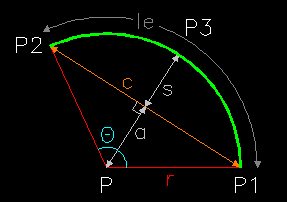
\includegraphics[width=0.5\textwidth]{figures/arcgeom.png}
	\captionof{figure}{Геометрия дуги окружности}
	\label{fig:arcgeom}
\end{figure}

Так как дуга окружности описывает часть этой окружности, то она и обладает всеми атрибутами данной окружности (см. рис. \ref{fig:arcgeom}). Среди них:

\begin{itemize}
	\item Радиус ($r$) --- радиус дуги такой же, как и у окружности;
	\item Центр ($P$) --- тот же, что и у окружности;
	\item Центральный угол ($\Theta$) --- в окружности равен $360^{\circ}$;
	\item Длина дуги ($le$) --- является частью периметра (длины) окружности.
\end{itemize}

Для дальнейшей работы с геометрией дуг примем, также, следующие специфичные атрибуты:

\begin{itemize}
	\item Начальная и конечная точка ($P1, P2$) --- это «вершины» дуги. Хотя иногда и целесообразно говорить о конкретных точках, не лежащих на концах дуги;
	\item Длина хорды ($c$) --- у дуг и окружностей можно провести бесконечное количество хорд, но для нас интерес представляет только хорда, проходящая через её вершины;
	\item Середина дуги ($P3$) --- точка, делящая дуги с данными вершинами на две, равные по длине, дуги;
	\item Апофема ($a$) --- это отрезок, вершинами которого являются середина дуги и её центр. Апофема перпендикулярна хорде;
	\item Высота дуги ($s$) --- это отрезок, проведённый из середины дуги перпендикулярно к хорде.
\end{itemize}

Кроме самой себя, дуга может, также, и описывать другие геометрические формы: круговой сегмент и сектор. Обе геометрические формы включают в себя все вышеперечисленные атрибуты, однако для выведения формулы параметра \textit{bulge} (выпуклости), потребуется рассмотрение только кругового сектора.

В документации AutoCAD \cite{autocad2012dxf} выпуклостью называется тангенс четверти угла дуги между выбранной вершиной и следующей вершиной в списках вершин полилиний. Отрицательность параметра \textit{bulge} указывает на то, что дуга отрисовывается по часовой стрелке от выбранной вершины к следующей. Выпуклость, равная нулю --- прямой сегмент, выпуклость, равная единице --- половина окружности.

Проблема «расшифровки» атрибутов дуги для дальнейших манипуляций с ней заключается в том, что входными данными являются только координаты вершин и рассматриваемый параметр --- \textit{bulge}.

В самом деле, взяв арктангенс от параметра \textit{bulge} и умножив его на $4$, легко получить центральный угол, на который опирается рассматриваемая дуга. Результат получен в радианах. Для перевода значения в градусы, необходимо умножить это значение на $\pi$ и разделить на $180^{\circ}$.

Для вывода данной зависимости, рассмотрим дугу окружности (см. рис. \ref{fig:arcchord}).

\begin{figure}[H]
	\centering
	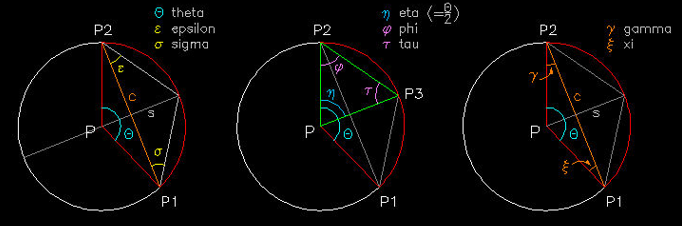
\includegraphics[width=1.0\textwidth]{figures/arcchord.png}
	\captionof{figure}{Дуга окружности с проведённой хордой и углами при ней}
	\label{fig:arcchord}
\end{figure}

Если провести к углу $\Theta$ биссектрису, то получится синий угол $\eta$. В итоге, мы получим равнобедренный треугольник (зеленый), в котором углы $\varphi$ и $\tau$ равны. Поскольку сумма углов в треугольнике всегда равна $180^{\circ}$ градусам, мы теперь знаем, что углы $\varphi$ и $\tau$ равны следующему (\ref{F:phi}):

\begin{equation}
	\varphi=\tau=\frac{(180^{\circ}-\frac{\Theta}{2})}{2}\Rightarrow\varphi=90^{\circ}-\frac{\Theta}{4}
	\label{F:phi}
\end{equation}

Теперь посмотрим на хорду $c$, проведённую от $P1$ до $P2$. Вместе с красными катетами угла $\Theta$ она тоже образует равнобедренный треугольник, а значит, $\gamma=\xi$. Угол при вершине треугольника $P-P1-P2$ --- это центральный угол $\Theta$, поэтому $\gamma$ и $\xi$ вычисляются следующим образом (\ref{F:gamma}):

\begin{equation}
	\gamma=\xi=\frac{180^{\circ}-\Theta}{2}\Rightarrow\gamma=90^{\circ}-\frac{\Theta}{2}
	\label{F:gamma}
\end{equation}

Таким образом, жёлтый угол $\varepsilon$ должен быть равняться разнице между фиолетовым углом $\varphi$ и оранжевым углом $\gamma$. Другими словами, $\varepsilon$ --- это четверть центрального угла $\Theta$ (\ref{F:epsilon}):

\begin{equation}
	\varepsilon=(90^{\circ}-\frac{\Theta}{4})-(90^{\circ}-\frac{\Theta}{2})\Rightarrow\varepsilon=\frac{\Theta}{2}-\frac{\Theta}{4}=\frac{\Theta}{4}
	\label{F:epsilon}
\end{equation}

Параметр \textit{bulge} (выпуклость) описывает, насколько дуга «выпирает» из вершин, то есть насколько велика высота дуги ($s$) (или расстояние от $P3$ до $P4$). Высота образует катет прямоугольного треугольника с углом, равным четверти центрального угла (см. жёлтый треугольник $P-P2-P3$ на рис. \ref{fig:epsilon}), и поскольку тангенс описывает отношение между катетами в прямоугольном треугольнике, легко описать геометрию с помощью этого одного угла (\ref{F:epsilon}):

\begin{equation}
	\frac{\sin(\varepsilon)}{\cos(\varepsilon)}=\tan(\varepsilon)
	\label{F:epsilon}
\end{equation}

\begin{figure}[H]
	\centering
	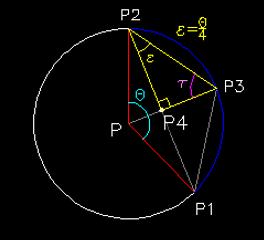
\includegraphics[width=0.5\textwidth]{figures/epsilon.png}
	\captionof{figure}{Связь угла $\varepsilon$ с центральным углом}
	\label{fig:epsilon}
\end{figure}

Мы, также, могли бы найти тангенс угла $\varepsilon$, просто разделив противолежащий катет на смежный катет --- что означает высоту дуги $s$, делённую на половину длины хорды $c$, --- но не зная $s$ и уже имея тангенс $\varepsilon$, полезнее найти $s$ (\ref{F:s}):

\begin{equation}
	s=\frac{c}{2}\cdot\tan(\varepsilon)
	\label{F:s}
\end{equation}

Примем

\begin{equation}
	\tan(\varepsilon)=bulge
	\label{F:tanepsilon}
\end{equation}

Тогда

\begin{equation}
	s=\frac{c}{2}\cdot bulge
	\label{F:sfinal}
\end{equation}

Таким образом, радиус дуги может быть найден следующим образом (\ref{F:r}):

\begin{equation}
	r=\frac{(\frac{c}{2})^2+s^2}{2s}
	\label{F:r}
\end{equation}

Знак той или иной выпуклости важен для определения дуги относительно вершин. Если выпуклость положительна, это означает, что дуга идёт против часовой стрелки от начальной вершины до конечной вершины. Если выпуклость отрицательна, это означает, что дуга идет, наоборот --- по часовой стрелке.

Поэтому все приведенные выше формулы должны касаться абсолютного значения выпуклости, а не фактического значения, иначе можно получить отрицательный радиус.

Итак, поняв, что $bulge = tan(\frac{\Theta}{4})$, в согласовании с документацией AutoCAD \cite{autocad2012dxf} примем, что \textit{bulge} положителен, когда при передвижении от начальной точки дуги к конечной движение происходит против часовой стрелки.

Ясно, что когда при $\Theta=0$ выпуклость $bulge(\Theta)=0$. Для углов в $180^{\circ}$: $bulge(\Theta)=\pm1$. В случае, когда $\Theta=90^{\circ}$, получим следующее (\ref{F:theta90}):

\begin{equation}
	bulge(90^{\circ})= \tan(\frac{90^{\circ}}{4})=\tan(\frac{\pi}{8})
	\label{F:theta90}
\end{equation}

Используя зависимость для тангенса половинного аргумента (\ref{F:tanhalfarg}):

\begin{equation}
	\tan(\frac{\alpha}{2})=\pm\frac{\sin(\frac{\alpha}{2})}{\cos(\frac{\alpha}{2})}=\pm\frac{2\sin^2(\frac{\alpha}{2})}{2\sin(\frac{\alpha}{2})\cos(\frac{\alpha}{2})}=\pm\frac{1-\cos(x)}{\sin(x)}
	\label{F:tanhalfarg}
\end{equation}

Для $\alpha=\frac{\pi}{8}$ получим (\ref{F:bulge90}):

\begin{equation}
	bulge(90^{\circ})=\tan(\frac{\pi}{8})=\pm\frac{1-\cos(\frac{\pi}{4})}{\sin(\frac{\pi}{4})}=\pm\frac{1-\frac{\sqrt2}{2}}{\frac{\sqrt2}{2}}=\pm\frac{1-\frac{1}{\sqrt2}}{\frac{1}{\sqrt2}}=\pm(\sqrt2-1)
	\label{F:bulge90}
\end{equation}



В результате, математические данные совпадают с документацией AutoCAD \cite{autocad2012dxf} и гласят, что

\begin{enumerate}
	\item $bulge = 0$ для отрезка прямой,
	\item $bulge = \pm1$ для дуги в $180^{\circ}$ (половина окружности),
	\item $bulge = \pm(\sqrt2-1) \approx0.41421...$ для четвертей окружностей, когда угол раствора дуги равен $90^{\circ}$.
\end{enumerate}

\section{Актуальное состояние проблемы использования файловых форматов в области САПР} \label{sec:actual}

САПР используют множество разных форматов хранения и передачи данных. Проблема заключается в унификации форматов с целью сокращения их числа и снижении нагрузки с процессов переконвертации и обработки различных форматов данных для получения необходимой информации внутри САПР.

Хотя задача полной унификации используемых форматов файлов вряд ли может быть полностью решена для современных  ПП, однако, в последние десятилетия развития технологий разработки программного обеспечения накоплены подходы, позволяющие значительно снизить остроту проблем, прежде всего за счёт продуманного использования открытых форматов хранения и обмена данными. При этом важны как функциональность формата, то есть то, какие именно данные он содержит, так и организация, то есть представление хранимых данных.

Например, для хранения и обмена геометрической информацией в САПР «Сириус» используется унаследованный двоичный формат DBS. Однако сложность чтения двоичного формата, неудобство хранения геометрической информации, а также актуальность акцент формата на экономии памяти препятствуют эффективной работе по обмену информацией между ПО. По этим причинам программистами САПР «Сириус» принято решение заменить данный формат другим --- более простым и удобным JSON.

На разных этапах как научных исследований, так и технологической подготовки производства, возникает потребность визуализации разнообразной геометрической информации, такой как геометрия деталей и ограничивающих их контуров, положение допустимых точек врезки и выключения инструмента, маршруты, получаемые в ходе решения различных классов задач резки, а также маршруты движения резака, получаемые после обработки постпроцессором и т.п.

Разработка в этих целях специальных графических утилит является традиционным подходом. Альтернативой, как пишет к.т.н. Уколов \cite{ukoloff}, является визуализация путём экспорта в удобочитаемый и поддерживаемый широкораспространёнными приложениями формат, например, в SVG. Векторные изображения, хранящиеся в этом формате, можно открывать с помощью любых современных браузеров; для формата доступно большое количество готовых библиотек; а также, формат кросс-платформенный, что означает возможность обозрения файлов данного типа на большинстве платформ и операционных систем.

В целях хранения промежуточных геометрических данных для дальнейшей обработки, а также для контроля содержания необходимых (поддерживаемых) примитивов (объектов) в DXF-файле, в рамках данной работы и проекта по разработке подсистем САПР \textit{ТокКТЭ} разработан новый формат хранения данных в текстовом документе --- TXT(DXF-type), который описан в разделе \ref{sec:aufgabe}. Также, с помощью данного формата может производится расчёт длины траектории  контура детали (обычно, в поперечном её сечении). Это может быть полезно при применении ПО в области лазерной резки с помощью станков с ЧПУ, а, в частности, в САПР <<Сириус>>.

В рамках этой работы и проекта по разработке подсистем САПР \textit{ТокКТЭ} был, также, изобретён формат хранения данных в текстовом файле --- TXT(x,y,r) в виде координат и радиуса (описание в разделе \ref{sec:aufgabe}). Он применяется для автоматизированного технологического проектирования, для формирования УП. Информация в данном формате о примитивах изображения контура детали используется для непосредственного составления УП, так как каждая последующая точка имеет не только плоские координаты, но и способ достижения этой точки (тип примитива: отрезок, если радиус равен нулю; дуга, если радиус ненулевой).

В целом, разрабатываемый набор конвертеров (модуль экспорта) представляет собой цельный ПП, сочетающий в себе набор необходимых разработчику УП начальных функций для автоматизированного технологического проектирования. Это ПО может быть интегрировано в подсистемы САПР по работе с файлами, так как по сути универсально в своём применении (используется в области 2D-резки, токарной обработке).

Несмотря на применимость в области САПР, приложение разрабатывалось с учётом возможности использования этого пользователями для их собственных целей, не связанных с САПР.


\section{Постановка задачи} \label{sec:aufgabe}

Необходимо разработать алгоритмы и приложение по конвертации данных из формата \textbf{DXF} в форматы \textbf{TXT (DXF-type)}, \textbf{TXT(x,y,r)}, \textbf{SVG}, \textbf{JSON}.

Формат TXT (DXF-type) должен содержать названия объектов (сущностей) с аттрибутом в скобках, под которыми они отображаются в DXF-формате (LINE, ARC и т.д.) в отдельных строках, после каждой из которых указываются основные параметры этих объектов. Для линий указываются координаты начала и конца. Для дуг и окружностей --- координаты центра и радиус. Для полилиний --- координаты точек, соединённых линиями. Например:
\begin{lstlisting}[label=list:dxftxtscheme]
LINE(#38)
156.732	67.105
124.332	67.105
ARC(#75)
-3.0	15.0	5.0
CIRCLE(#2B9)
0.0 0.0 20.0
LWPOLYLINE(#2A9)
0.0 0.0 10.0 0.0 10.0 10.0 0.0 10.0 
\end{lstlisting}

Формат выходного файла TXT(x,y,r) содержит в каждой строке по три параметра: координата абсциссы точки, координата ординаты и радиус перехода от данной точки к следующей (последний \textit{bulge} DXF-файла, при незамкнутом контуре полилинии, не имеет смысла). Пример содержания такого файла:
\begin{lstlisting}[label=list:dxftxtscheme]
158.33 59.61 0
108.33 59.61 0
108.33 78.61 0
118.33 68.11 0
120.33 66.11 2.00
\end{lstlisting}

Формат SVG стандартизован (см. раздел \ref{subs:svg}). При его открытии любым из доступных способов (с помощью Интернет-браузера, например) должно корректно отображаться поддерживаемые объекты входного DXF.

Формат JSON так же стандартизован (раздел \ref{subs:json}), однако после конвертации файлы в этом формате должны содержать данные по двум тэгам: \textit{partid} и \textit{paths}, например:
\begin{lstlisting}[language=json,label=list:dxftxtscheme]
[{
	"partid": "LIST",
	"paths": [
	[
	[0, 0, 0],
	[0, 2000, 0],
	[5000, 2000, 0],
	[5000, 0, 0],
	[0, 0, 0]]
	]},{
	"partid": "00112",
	"paths": [
	[
	[322, 1045, 1],
	[448, 1045, 1],
	[322, 1045, 0]],
	[
	[72, 1045, 1],
	[198, 1045, 1],
	[72, 1045, 0]],
	[
	[197, 785, 1],
	[323, 785, 1],
	[197, 785, 0]]
	]}
\end{lstlisting}

Здесь в тэге \textit{pathid} указывается наименование детали, а в тэге \textit{paths} --- примитивы, задающиеся по типу TXT(DXF-type).

Схема работы приложения представлена на рисунке \ref{fig:primiviewscheme}.

\begin{figure}[H]
	\centering
	\includegraphics[width=1.0\textwidth]{figures/primiviewscheme.png}
	\captionof{figure}{Схема работы разрабатываемого ПО}
	\label{fig:primiviewscheme}
\end{figure}

Кроме конвертации данных, необходимо предусмотреть в приложении визуализацию прочитанных из DXF-файла геометрических данных для проверки корректности чтения их программой (т.е. для верификации).

\paragraph{Главные требования ко входному DXF-файлу}

Так как данная работа нацелена на создание ПО для обработки геометрической информации 2D-объектов \textbf{специального типа}, то конвертироваться из DXF-файлов должна не вся информация, содержащаяся в них. В первую очередь, заказчиком работы было определено, что на входе будет подаваться \textbf{2D-контур} деталей типа <<Втулка>>, то есть \textbf{тел вращения}. Так как сконвертированная геометрия данных объектов в последующем предполагает разработку УП для токарных станков с ЧПУ, то геометрическая информация должна содержать определённый набор геометрических примитивов, с которым может работать система исполнительных органов станков с ЧПУ. Этот набор ограничивается тем, что исполнительные органы станков с ЧПУ способны перемещаться либо с помощью \textbf{линейной}, либо с помощью \textbf{круговой интерполяции}. Из этого следует, что для корректной работы САПР, для которых предназначаются разрабатываемые конвертеры, геометрия в DXF-файле на входе конвертеров должна состоять из, как минимум одного из представленных далее примитивов:

\begin{enumerate}
	\item линия (отрезок),
	\item полилиния,
	\item дуга,
	\item окружность.
\end{enumerate}

Остальные типы геометрии, реализуемой в формате DXF, такие как \textit{эллипс}, \textit{сплайн}, будут игнорироваться ПО.

На вход разрабатываемому конвертеру подаётся файл формата DXF. Формат DXF представляет собой совокупность данных с тегами всей информации, содержащейся в файле чертежа AutoCAD. Тегированные данные означают, что каждому элементу данных в файле предшествует целое число, называемое групповым кодом. Значение группового кода указывает, какой тип данных имеет следующий элемент. Это значение также указывает смысл элемента данных для данного типа объекта. Практически вся указанная пользователем информация в файле чертежа может быть представлена в формате DXF \cite{autocad2012dxf}.
В DXF файлах, в зависимости от их содержания, существуют сущности, представляющие для нас интерес. Среди них следующие:

\begin{enumerate}
	\item LINE (Линия),
	\item LWPOLYLINE (Полилиния),
	\item ARC (Дуга),
	\item CIRCLE (Окружность),
	\item INSERT (Вставка).
\end{enumerate}

Как уже и было отмечено, существуют и другие примитивы (ELLIPSE, SPLINE и др.), однако, основываясь на конкретных целях заказчика по возможности применения выходных файлов для генерации УП, ПП проектируется только с указанными примитивами и сущностями DXF.

Рассмотрим каждую из сущностей подробнее.

\paragraph{LINE.} Рассмотрим тэги сущности \textit{Линия}, необходимые для её реального отображения (см. табл. \ref{tab:line}).


\begin{longtable}{|l|l|}
	\caption{Рассматриваемые групповые коды сущности LINE}
	\label{tab:line}
	\centering
	\tabularnewline
	\hline
	Групповой код & Описание\\
	\hline \endfirsthead
	\subcaption{Продолжение таблицы~\ref{tab:line}}
	\\ \endhead
	\subcaption{Продолжение на след. стр.}
	\endfoot
	%\hline
	\endlastfoot
	39	&	Толщина (необязательный; по умолч. = 0)\\ \hline
	10	&	Начальная точка (в с.к. объекта) DXF: значение X\\ \hline
	20, 30	&	DXF: Y и Z значения начальной точки (в с.к. объекта)\\ \hline
	11	&	Конечная точка (в с.к. объекта)	DXF: значение X\\ \hline
	21, 31	&	DXF: Y и Z значения конечной точки (в с.к. объекта)\\ \hline
\end{longtable}

\paragraph{LWPOLYLINE.} Рассмотрим тэги сущности \textit{Полилиния}, необходимые для её реального отображения (см. табл. \ref{tab:polyline}).

\begin{longtable}{|p{70pt}|p{370pt}|}
	\caption{Рассматриваемые групповые коды сущности POLYLINE}
	\label{tab:polyline}
	\centering
	\tabularnewline
	\hline
	Групповой код & Описание\\
	\hline \endfirsthead
	\subcaption{Продолжение таблицы~\ref{tab:polyline}}
	\\ \endhead
	\subcaption{Продолжение на след. стр.}
	\endfoot
	%\hline
	\endlastfoot
	70	&	«Флаг» полилинии (бит-закодировано); по умолч. = 0; 1 – закрыта\\ \hline
	39	&	Толщина (необязательный; по умолч. = 0)\\ \hline
	10	&	Координаты вершин (в с.к. объекта), множественные вхождения; по одному вхождению для каждой вершины DXF: значение X\\ \hline
	20	&	DXF: значение Y координат вершин (в с.к. объекта), множественные вхождения; по одному вхождению для каждой вершины\\ \hline
	42	&	\textit{Bulge}. Выпуклость (множественные вхождения - для каждой вершины), (необязательно; по умолч. =0)\\ \hline	
\end{longtable}

\paragraph{ARC.} Рассмотрим тэги сущности \textit{Дуга}, необходимые для её реального отображения (см. табл. \ref{tab:arc}).

\begin{longtable}{|p{70pt}|p{370pt}|}
	\caption{Рассматриваемые групповые коды сущности ARC}
	\label{tab:arc}
	\centering
	\tabularnewline
	\hline
	Групповой код & Описание\\
	\hline \endfirsthead
	\subcaption{Продолжение таблицы~\ref{tab:arc}}
	\\ \endhead
	\subcaption{Продолжение на след. стр.}
	\endfoot
	%\hline
	\endlastfoot
	39	&	Толщина (необязательный; по умолч. = 0)\\ \hline	
	10	&	Центр дуги (в с.к. объекта)
	DXF: значение X\\ \hline	
	20, 30	&	DXF: Y и Z значения центра дуги (в с.к. объекта)\\ \hline	
	40	&	Радиус\\ \hline	
	50	&	Начальный угол\\ \hline	
	51	&	Конечный угол\\ \hline	
\end{longtable}

\paragraph{CIRCLE.} Рассмотрим тэги сущности \textit{Окружность}, необходимые для её реального отображения (см. табл. \ref{tab:circle}).

\begin{longtable}{|p{70pt}|p{370pt}|}
	\caption{Рассматриваемые групповые коды сущности CIRCLE}
	\label{tab:circle}
	\centering
	\tabularnewline
	\hline
	Групповой код & Описание\\
	\hline \endfirsthead
	\subcaption{Продолжение таблицы~\ref{tab:circle}}
	\\ \endhead
	\subcaption{Продолжение на след. стр.}
	\endfoot
	%\hline
	\endlastfoot
	39	&	Толщина (необязательный; по умолч. = 0)\\ \hline	
	10	&	Центр дуги (в с.к. объекта)
	DXF: значение X\\ \hline	
	20, 30	&	DXF: Y и Z значения центра дуги (в с.к. объекта)\\ \hline	
	40	&	Радиус\\ \hline	
	50	&	Начальный угол\\ \hline	
	51	&	Конечный угол\\ \hline	
\end{longtable}

\paragraph{INSERT.} Данная сущность представляет собой вставку блоков с геометрией. Её необходимо рассматривать, так как геометрия может быть вложенной и, таким образом, не видна обзорщиком сущностей, так как вложена. У этой сущности поиск информации по тэгам в программе не потребуются.


\section{Выводы по главе \ref{cha:aktuell}}
Анализ состояние вопросов конвертации данных и графических файлов DXF показал, что:
\begin{itemize}
	\item Задача по конвертации данных из разных форматов с целью обмена графической информацией в САПР сложна и требует, как специальных знаний в области изучаемых форматов, так и опыт в разработке алгоритмов и ПО по ним для САПР;
	\item Существующие предложения открытого рынка по ПП, конвертирующим DXF файлы. Однако эти решения не удовлетворяют потребностям, предъявляемым к выходным форматам данных;
	\item Для корректной работы программы, разработчику алгоритмов и ПО необходимы знания геометрии примитивов (в особенности, дуг), с которыми ведётся работа.	
\end{itemize}

\chapter{Разработка файловых конвертеров в виде приложения <<primiview>>}
\label{cha:entwickl}

Программное обеспечение решено назвать \textbf{<<primiview>>}, где \textbf{<<primi>>} --- сокращение от англ. \textit{primitive} (\textit{примитив}), \textbf{view} --- в переводе с англ. \textit{обзор}.

В данном разделе описаны экономические аспекты проекта по созданию ПО <<primiview>> для обработки геометрической информации 2D-объектов специального типа.

\section{Выбор языка программирования}
Для написания программы выбран язык программирования Python версии 3.11. Выбор языка программирования обоснован несколькими факторами.

\paragraph{Библиотеки.} Для создания описанного ПП необходимо привлечение различных библиотек. Кроме стандартной библиотеки, с Python можно использовать множество прикладных библиотек, несколько из которых будут описаны в следующих частях работы. Специфичные библиотеки, позволяющие <<читать>> DXF-файл и обрабатывать содержимое внутри него, написаны не для каждого ЯП. Библиотека <<eazy dxf>> для Python позволяет быстро и удобно выполнять данные операции.

\paragraph{Кроссплатформенность.} Большинство программ, написанных на Python, выполняются корректно на всех основных платформах. Перенос программы между операционными системами реализуется простым копированием кода. Кроме того, в процессе разработки ПО, для реализации пользовательского интерфейса используется набор расширений Qt, который тоже работает на таких платформах, как Linux и другие UNIX-подобные ОС, macOS и Windows.

\paragraph{Скорость и удобство разработки.} Удобочитаемсть, ясность и высокое качество этого языка позволяют повысить производительность разработчика во много раз, сравнивая, например, с компилирующими или строго типизированными языками, такими как C, C++ и Java. Объём программного кода на языке Python обычно составляет треть или даже пятую часть эквивалентного программного кода на языке C++ или Java. Кроме того, при запуске программы, написанной на ЯП Python минуются длинные этапы компиляции и связывания, необходимые в некоторых других ЯП, что, также, увеличивает производительность труда программиста \cite{ascher2004learning}.

В ходе сравнительного анализа языков программирования для использования особое внимание уделялось чтению DXF. В тоткрытом доступе были найдены библиотеки для Python (\textit{ezdxf}), C\#(\textit{netDxf}), для C++ и других языков были найдены исходные коды, позволяющие обрабатывать DXF-файлы.

В итоге, учитывая вышеприведённые аспекты-преимущества языка Python, а также относительно большой опыт работы по написанию ПО на этом языке, в сравнении с другими, учитывая крайне высокую степень разработки библиотеки \textit{ezdxf} было принято решение использовать язык Python и библиотеку \textit{ezdxf} для разработки ПО.


\section{Принцип работы приложения <<primiview>>}

Для создания программного обеспечения необходимо сначала разработать концепцию функционирования программы, опираясь на её назначение, на основные её функции. Когда определены модули, блоки и функциональные части ПО, можно приступать к разработке его на выбранном ЯП.

Основываясь на цели, поставленной во введении, разрабатываемая утилита должна принимать на входе DXF-файл, то есть открывать его и обрабатывать его содержимое. Для проверки правильности обработанных данные, то есть, для верификации содержимого DXF-файла, программа должна визуализировать для пользователя обработанное. После верификации обработанных данных и, соответственно, подтверждения соответствия их исходным, пользователю должна предоставляться возможность конвертировать эти данные в какой-либо из предлагаемых форматов. За это отвечает модуль экспорта, который, в свою очередь, подразделяется на четыре модуля, отвечающие за преобразование данных в различные форматы. Среди них следующие:

\begin{enumerate}
	\item Модуль экспорта в TXT-файл, где данные будут представлены в такой же форме, как и в оригинальном DXF-файле, за исключением того, что содержаться в нём будут только поддерживаемые сущности (LINE, POLYLINE, ARC, CIRCLE).
	\item Модуль экспорта в TXT-файл, в котором поддерживаемые сущности будут представлены сочетанием двух строк, первая из которых --- начальная точка примитива, вторая --- конечная. Вторая строка содержит в себе радиус скругления примитива, переходящего из первой точки во вторую.
	\item Модуль экспорта в формат SVG, который, при открытии, векторно отображает информацию в нём.
	\item Модуль экспорта JSON-формат. В данном формате, по подобию формату TXT (x, y, r), содержаться точки, олицетворяющие начало и конец того или иного примитива. В данном случае информация в файле тэгированная, что означает, что в дальнейшем несложно будет получить желаемые куски данных из потенциально объёмного JSON-файла путём обращения по желаемому тэгу.
\end{enumerate}


Схему, отображающую основное содержание разрабатываемого ПО, можно наблюдать на рисунке \ref{fig:organisationsdiagramm}.

\begin{figure}[H]
	\centering
	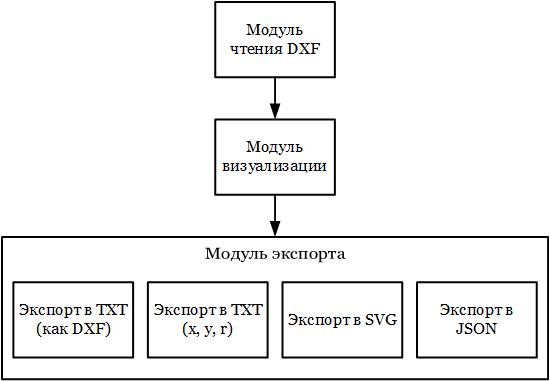
\includegraphics[width=0.8\textwidth]{figures/organisationsdiagramm.png}
	\captionof{figure}{Принципиальная структура ПО <<Primiview>>}
	\label{fig:organisationsdiagramm}
\end{figure}

\section{Внутрепрограммная репрезентация информации о геометрических примитивах}
Учитывая то, что проблема с работой по чтению входных DXF-файлов решена с помощью библиотеки \textit{ezdxf}, задача разработки ПО фактически свелась к внутренней респезентации необходимой геометрической информации внутри программы для дальнейшей работы с ней.

Есть несколько вариантов хранения геометрических данных в программе на ЯП Python: списки, словари и классы.

В списках обычно хранятся объекты одного типа (например, только координаты в виде чисел). Это не удовлетворяет потребности обмена данными, так как нужная геометрическая информация из DXF содержит в себе и строковые, и булевы значения, а также другие типы данных.

Словари обеспечивают более простой и понятный доступ к полям, чем списки (то есть не по числовым индексам, а по ключам). Однако словари имеют некоторые ограничения, которые могут оказаться существенными по мере разработки программы.

Во-первых, в словарях не предусмотрено место для централизованного хранения логики обработки записей. Это допустимо в разрабатываемом ПО, так как функции работы с геометрическими примитивами в частях программы имеют одинаковый характер, поэтому не требуется прописывать поведение каждого класса объектов \cite{lutz2001programming}.

Однако недостаток использования словарей для представления записей, заключающийся в том, что со временем их становится трудно расширять, является решающим при выборе типа данных для хранения информации о геометрических примитивов. Так как ПО <<primiview>> требуется постоянно модифицировать для работы с новыми файловыми форматами, то основные изменения исходят из взятия из исходных DXF-файлов дополнительной информации для её последующей обработки. Поэтому сложность дополнения словарей новой информацией недопустима при разработке данного ПО.

Кроме прочих преимуществ хранения данных с помощью классовых свойств, ценна возможность создания списков внутри классов, которые позволяют объединять одноротную по типу информацию, что упрощает её дальнейшую обработку.

Таким образом, учитывая вышеприведённые аргументы, а также следуя принципам объектно-ориентированного программирования (ООП) в разработке ПО, принято решение хранить каждый примитив в виде объекта класса этих примитивов.

Предусмотрен отдельный класс данных (\textit{DxfData}), работающий с примитивами, извлечёнными из DXF. Он содержит в себе списки объектов соответствующих классов (линия, дуга, др.), а также методы (функции внутри класса) по работе с ними.

Схема, отображающая структуру хранения данных из DXF-файлов внутри программы приведена на рисунке \ref{fig:classes}.

\begin{figure}[H]
	\centering
	\includegraphics[width=1.0\textwidth]{figures/classes.png}
	\captionof{figure}{Структура хранения данных в ПО <<primiview>>}
	\label{fig:classes}
\end{figure}


\section{Разработка алгоритмов} \label{sec:algs}
Алгоритм \ref{alg:readdxf} показывает схему работы процесса извлечения поддерживаемых ПО Primiview примитивов из выбранного DXF-файла.

На первой итерации осуществляется разбиение блоков, в которых могут быть <<спрятаны>> остальные сущности. В случае, если пропустить данный этап, то объекты, находящиеся внутри блоков не будут видны библиотекой \textit{ezdxf}, которая используется для чтения DXF-файлов.

После <<разрушения>> всех блоков примитивы становятся <<видимыми>>. Далее запускается цикл, итерирующий объекты пространства объектов модели (\textit{modelspace}). В случае совпадения объекта с одной из поддерживаемых сущностей, она сохраняется в список соответствующих объектов в оперативной памяти программы. Списком далее будет называться изменяемый упорядоченный тип данных, представляющих собой последовательность элементов, разделённых между собой запятой и заключённых в квадратные скобки. Данный тип данных используется в ЯП Python.

Примем ряд условных обозначений:

$\rightsquigarrow$ --- запись в файл;
$\dashrightarrow$ --- запись объекта в множество.


\begin{algorithm}[H]
	\SetAlgoLined
	\KwData{путь к DXF-файлу}
	\KwResult{массивы примитивов и информации о них в оперативной памяти программы}
	инициализация;
	
	\ForEach{объекта типа Вставка (INSERT) $\in msp$}{разбиение сущности}
	
	\ForEach{объекта $\in msp$}{
		\If{объект явл. линией}{объект. $\dashrightarrow$ множ. линий}
		\ElseIf{объект явл. дугой}{объект $\dashrightarrow$ множ. дуг}
		\ElseIf{объект явл. окружностью}{объект $\dashrightarrow$ множ. окружностей}
		\ElseIf{объект явл. полилинией}{объект $\dashrightarrow$ множ. полилиний}
	}
	
	\caption[Сохранение поддерживаемых примитивов; из DXF в оперативную память программы]
	{\tabular[t]{@{}l@{}}Сохранение поддерживаемых примитивов \\ из DXF в оперативную память программы\endtabular}
	\label{alg:readdxf}
\end{algorithm}

\paragraph{Алгоритм записи примитивов в TXT (как DXF).} Принцип данного алгоритма (см. алгоритм \ref{alg:dxfintotxt}) основан на открытии созданного TXT-файла, а после --- перебора прочитанных из DXF примитивов и записи из каждого из них необходимой информации в открытый для редактирования TXT-файл.

Записи в текстовом файле должны выглядеть следующим образом (см. листинг \ref{list:txtdxfsicht}):
%\begin{verbatim}
%	LINE(#01)
%	0.1 0.1
%	0.1 0.1
%\end{verbatim}

\begin{lstlisting}[caption={Пример содержания TXT-файла (как DXF)},label=list:txtdxfsicht]
	LINE(#01)
	0.1 0.1
	0.1 0.1
\end{lstlisting}

\begin{algorithm}[H]
	\SetAlgoLined
	\KwData{данные из DXF, путь к имя.txt}
	\KwResult{имя.txt (как DXF)}
	инициализация;
	\ForEach{LINE}{атрибут сущности, $x_0, y_0$, $x_1, y_1 \rightsquigarrow$имя.txt}
	\ForEach{ARC}{атрибут сущности, $x_0, y_0$, $x_1, y_1$, $r\rightsquigarrow$имя.txt}
	\ForEach{CIRCLE}{атрибут сущности, $x_c, y_c$, $r\rightsquigarrow$имя.txt}
	\ForEach{LWPOLYLINE}{атрибут сущности;\\
		\ForEach{LWPOLYLINE}{
			\ForEach{координата}{координата$\rightsquigarrow$имя.txt}
		}}
	\caption{Запись примитивов в TXT (DXF-type)}
	\label{alg:dxfintotxt}
\end{algorithm}

В алгоритме \ref{alg:dxfintotxt} $x_0, y_0$ --- координаты начала примитива; $x_1, y_1$ --- координаты конца примитива; $x_c, y_c$ --- координаты центра окружности; $r$ --- радиус дуги или окружности.

\paragraph{Алгоритм записи примитивов в TXT (x,y,r).} Алгоритм \ref{alg:primsintotxt} призван, так же как и в прошлом случае, в открытый только что созданный текстовый файл записать информацию о примитивах, которые были прочитаны из выбранного DXF-файла.

Записи в текстовом файле должны выглядеть следующим образом (см. листинг \ref{list:primsdxfsicht}):
%\begin{verbatim}
%	1.52 1.86 0
%	1.12 2.08 0
%	1.16 2.04 4.0
%	...
%\end{verbatim}

\begin{lstlisting}[caption={Пример содержания TXT-файла (x, y, r)},label=list:primsdxfsicht]
	1.52 1.86 0
	1.12 2.08 0
	1.16 2.04 4.0
\end{lstlisting}

Полилиния может содержать в себе, как отрезки, так и дуги. В объектах LWPOINT сущности LWPOLYLINE степень искривления показывает параметр \textit{bulge}, суть которого подробно описана в разделе \ref{sec:arcs}. Так как желаемый формат вывода информации о примитивах содержит именно радиус примитива, а не параметр искривления, то необходимо удобно получить радиус из \textit{bulge}.

Для этого воспользуемся уже выведенной зависимостью \cite{ukoloff} и применим её в принятых обозначениях (\ref{F:rad}):

\begin{equation}
	R=|bulge+\frac{1}{bulge}|\cdot\frac{|A-Z|}{4},
	\label{F:rad}
\end{equation}

где A --- начальная точка;

Z --- конечная точка.

Примем, что $A(x_0,y_0), B(x_1,y_1)$. Тогда $AZ(x_1-x_0; y_1-y_0)$.
Таким образом, длина вектора через декартовы координаты (\ref{F:veclen}):
\begin{equation}
	|A-Z|=\sqrt{(x_1-x_0)^2+(y_1-y_0)^2}
	\label{F:veclen}
\end{equation}


\begin{algorithm}[H]
	\SetAlgoLined
	\KwData{текущая точка, следующая точка}
	\KwResult{радиус сегмента полилинии}
	инициализация;
	
	\If{$bulge$ (текущей точки) $=0$}{$r=0$}	
	\Else{$r=|bulge+\frac{1}{bulge}|\cdot\frac{\sqrt{(x_{nexP}-x_{prevP})^2+(y_{nexP}-y_{prevP})^2}}{4}$}
	
	\caption{Вычисление радиуса сегмента полилинии}
	\label{alg:polyarcrad}
\end{algorithm}

\begin{algorithm}[H]
	\SetAlgoLined	
	\KwData{данные из DXF, путь к имя.txt}
	\KwResult{имя.txt (x,y,r)}	
	\ForEach{LINE}{$x_0 \quad y_0 \quad 0\rightsquigarrow$ имя.txt; \quad $x_1 \quad y_1 \quad 0 \rightsquigarrow$ имя.txt}
	
	\ForEach{ARC}{$x_0 \quad y_0 \quad 0\rightsquigarrow$ имя.txt; \quad $x_1 \quad y_1 \quad r \rightsquigarrow$ имя.txt}
	
	\ForEach{CIRCLE}{$x_c + r \quad y_c \quad 0\rightsquigarrow$ имя.txt\tcc*{первая половина окруж.} $x_c - r \quad y_c \quad r \rightsquigarrow$ имя.txt \\  $x_c - r \quad y_c \quad 0 \rightsquigarrow$ имя.txt\tcc*{вторая половина окруж.} $x_c + r \quad y_c \quad r \rightsquigarrow$ имя.txt} \ForEach{POLYLINE\\ prevPoint=None \tcc*{предыдущая точка}}{
		\ForEach{LWPOINT $\in$ множ. точек полилинии}{
			\If{prevPoint$\neq$None}{r = алгоритм \ref{alg:polyarcrad} (prevPoint, LWPOINT)
				$x(prevP) \quad y(prevP) \quad 0 \rightsquigarrow$ имя.txt\\
				$x(lwpoint) \quad y(lwpoint) \quad r \rightsquigarrow$ имя.txt
			}
			$prevPoint = lwpoint$
		} \newpage
		\If{контур замкнут}{
			r = алгоритм \ref{alg:polyarcrad} (prevPoint, LWPOINT) \\
			$x(lwpoint_\text{посл}) \quad y(lwpoint_\text{посл}) \quad 0 \rightsquigarrow$ имя.txt\\
			$x(lwpoint_\text{перв}) \quad y(lwpoint_\text{перв}) \quad r \rightsquigarrow$ имя.txt
		}
	}
	\caption{Запись примитивов в TXT (x, y, r)}
	\label{alg:primsintotxt}
\end{algorithm}

\paragraph{Алгоритм записи примитивов в SVG.} Формирования файла типа SVG отличается от предыдущих двух, так как этот формат представляет собой язык разметки, а значит, имеет правила синтаксиса, грамматики и т.д. Это расширение языка разметки XML, поэтому в начале, в преамбуле, указывается версия XML, кодировка символов и указание синтаксическому анализатору об игнорировании любых объявлений разметки в определении типа документа.

\begin{lstlisting}[language=XML,caption={Первая строка SVG-файлов},label=list:1stsvgline]
	<?xml version="1.0" encoding="UTF-8" standalone="no"?>
\end{lstlisting}

Следующие две строки должны содержать определение типа документа (заголовок DOCTYPE), однако, данное объявление может оказаться источником ошибок при применении в браузере Mozilla Firefox. Поэтому вместо этого используется атрибут \Code{baseProfile} со значением <<full>> внутри элемента <svg>.

Начиная с четвёртой строки объявляется корневой элемент <svg>:

\begin{lstlisting}[language=XML,caption={Первая строка SVG-файлов},label=list:4thsvgline]
	<svg version="1.1" width="100%" height="100%"
	viewBox="102.1188828597992 -211.7921423734452 50.000000000000014 26.0"
	baseProfile="full"
	xmlns="http://www.w3.org/2000/svg"
	xmlns:xlink="http://www.w3.org/1999/xlink"
	xmlns:ev="http://www.w3.org/2001/xml-events">
\end{lstlisting}

В листинге \ref{list:4thsvgline} присутствует необязательный элемент \Code{viewBox}, который представляет собой параметр с четырьмя значениями, отделяемыми пробелами, определяющими квадратную рамку, в которой будет располагаться графика. Данный атрибут позволяет автоматически масштабировать изображение до размеров указанного контейнера, причём, без потери качества, так как графическая информация храниться и воспроизводится в векторном формате.

Первые два значение --- минимальные координаты $x$ и $y$ рамки, в которой располагается изображение. Третье и четвёртое значения --- соответственно, ширина и высота рамки, в которой находится изображение. Значения указываются в пикселях.

Таким образом, чтобы перенести данные из DXF в SVG, сначала определяются эти четыре значения. Алгоритмы для их определения: алгоритм \ref{alg:allcoords}, алгоритм \ref{alg:extremums} и алгоритм \ref{alg:dimes}.

\begin{algorithm}[H]
	\SetAlgoLined
	\KwData{списки примитивов с параметрами}
	\KwResult{список координат $x$, список координат $y$}
	инициализация; пустой список координат $x$, пустой список координат $y$
	
	\ForEach{LINE}{$x_0,x_1\dashrightarrow$ список $x$\\$y_0,y_1\dashrightarrow$ список $y$}
	
	\ForEach{ARC}{$(x_c+r),(x_c-r)\dashrightarrow$ список $x$\\$(y_c+r),(y_c+r)\dashrightarrow$ список $y$}
	
	\ForEach{CIRCLE}{$(x_c+r),(x_c-r)\dashrightarrow$ список $x$\\$(y_c+r),(y_c+r)\dashrightarrow$ список $y$}
	
	\ForEach{LWPOLYLINE}{
		\ForEach{точки $\in$ множ. LWPOINTS}{
			$x\dashrightarrow$ список $x$\\$y\dashrightarrow$ список $y$}}
	вернуть список координат $x$ и список координат $y$
	\caption{Вычленение координат изображения из DXF в отдельные списки}
	\label{alg:allcoords}
\end{algorithm}

\begin{algorithm}[H]
	\SetAlgoLined
	\KwData{список координат $x$, список координат $y$}
	\KwResult{$x_{MIN}, y_{MIN}$}
	инициализация;\\
	использовать алгоритм \ref{alg:allcoords}\\
	вернуть $x_{MIN}, y_{MIN}$ из списков стандартными функциями сортировки ЯП
	\caption{Поиск наименьших координат изображения из DXF}
	\label{alg:extremums}
\end{algorithm}

\begin{algorithm}[H]
	\SetAlgoLined
	\KwData{список координат $x$, список координат $y$}
	\KwResult{ширина и высота рамки изображения}
	инициализация;
	использовать алгоритм \ref{alg:allcoords}\\
	определить $x_{MIN}, x_{MAX}, y_{MIN}, y_{MAX}$ из списков стандартными методами сортировки множеств, встроенными в ЯП\\
	ширина $=x_{MAX}-x_{MIN}$\\
	высота $=y_{MAX}-y_{MIN}$\\
	вернуть значения ширины и высоты
	\caption{Поиск длины и высоты изображения из DXF}
	\label{alg:dimes}
\end{algorithm}

\paragraph{Алгоритм разбиения полилинии}
В процессе разработки приложения возникает задача визуализации данных из DXF. Проблемы возникают только с объектом Полилиния, который задаётся в DXF компактно: с помощью параметра \textit{bulge}. Библиотека отрисовки в используемом ЯП, однако, не позволяет задавать полилинии ни в каком виде. По этой причине полилинию необходимо разбивать на линии и дуги по алгоритму \ref{alg:polytolinearcs}.

В алгоритме происходит перемена углов дуги местами, если параметр кривизны меньше нуля. Это происходит потому, что в библиотеке \textit{matplotlib} направление отрисовки дуг, как и в AutoCAD, всегда по часовой стрелке. А значит, что регулировка <<величины>> дуги регулируется последовательностью указания углов её отрисовки.

\begin{algorithm}[H]
	\SetAlgoLined
	\KwData{список Полилиний с lwpoints у каждой}
	\KwResult{линия/дуга}
	инициализация;
	\ForEach{POLYLINE}{
		\ForEach{текущая т., след. т.}{
			\If{$bulge=0$}{рисуй линию с соотв. коор.}
			\Else{
				центр, радиус = алгоритм \ref{alg:polyarc_center_rad} (текущая т., след. т.)\\
				нач.угол. = алгоритм \ref{alg:angle_vectors} (тек.т., центр)\\
				конеч.угол. = алгоритм \ref{alg:angle_vectors} (след.т., центр)
				\If{$bulge<0$}{поменять местами углы}
				рисуй дугу с соотв. центром, радиусом и углами.
			}
		}
	}
	\caption{Разбиение полилиний для визуализ. primiview}
	\label{alg:polytolinearcs}
\end{algorithm}

В работе Уколова С.С. \cite{ukoloff} выведена зависимость, связывающая параметр \textit{bulge},  \textit{комплексное} представление координат точек начала ($A$) и конца ($Z$) дуги с координатами центра ($C$) дуги:
\begin{equation}
	C={\frac{(1+ibulge)^2}{4ibulge}}\cdot A-{\frac{(1-ibulge)^2}{4ibulge}}\cdot Z
	\label{F:arcenter}
\end{equation}

\begin{algorithm}[H]
	\SetAlgoLined
	\KwData{тек.т., след.т.}
	\KwResult{коор.центра дуги, радиус}
	инициализация;\\
	$A=x+iy$ (тек.т.)\\
	$Z=x+iy$ (след.т.)\\
	$C={\frac{(1+ibulge)^2}{4ibulge}}\cdot A-{\frac{(1-ibulge)^2}{4ibulge}}\cdot Z$ ($bulge$ текущей точки, см. раздел \ref{sec:aufgabe})\\
	$rad=$ алгоритм \ref{alg:polyarcrad}\\
	верни C(действ.ч., мним.ч.), радиус
	\caption{Вычисление координат центра и радиуса дуги}
	\label{alg:polyarc_center_rad}
\end{algorithm}

Угол между векторами ищется с помощью известной арктангенса от частного состовляющих $y$ и $x$ координат, соответственно. Результат находится в диапазоне $\pm\pi$, поэтому после этого берется остаток от деления на $360^\circ$.

\begin{algorithm}[H]
	\SetAlgoLined
	\KwData{точка дуги, центр дуги}
	\KwResult{угол от полож. направ. $Ox$}
	инициализация;\\
	$vector=\text{точка дуги}-\text{центр дуги}$\\
	$vecOx$ --- вектор положительного направления $Ox$\\
	$\alpha=\frac{\arctan(\frac{vector}{vecOx})\cdot\frac{180}{\pi}}{360}$\\
	верни $\alpha$
	\caption{Угол между векторами}
	\label{alg:angle_vectors}
\end{algorithm}

Итак, алгоритм \ref{alg:svg} --- формирование SVG-файла.

\begin{algorithm}[H]
	\SetAlgoLined
	\KwData{путь к имя.svg}
	\KwResult{имя.svg}
	инициализация;\\
	открой имя.svg\\
	преамбула (см. раздел \ref{subs:svg}) $\rightsquigarrow$ имя.svg\\
	\ForEach{LINE}{$x_0, y_0\rightsquigarrow$ имя.svg\\
		$x_1, y_1\rightsquigarrow$имя.svg}
	\ForEach{ARC}{
	размер дуги = малая, поворот дуги = по час.\\
	\If{$(\alpha_1-\alpha_0) / 360 > 180$}{размер дуги = большая}
	$x_0, y_0, r\rightsquigarrow$ имя.svg\\
	размер дуги, поворот дуги,$x_1, y_1\rightsquigarrow$имя.svg
	}
	\ForEach{CIRCLE}{$x_c, y_c, r\rightsquigarrow$ имя.svg}
	\ForEach{POLYLINE}{список points\\
		\ForEach{LWPOINT}{points$\dashrightarrow$список points}
		\ForEach{point}{$point_0, point_1 \rightsquigarrow$имя.svg}
	}
	\caption{Запись примитивов в SVG}
	\label{alg:svg}
\end{algorithm}

Алгоритм, совмещенный из \ref{alg:json}, \ref{alg:json1}, используется для создания JSON-файла с содержанием из исходного DXF.

\begin{algorithm}[H]
	\SetAlgoLined
	\KwData{путь к имя.json}
	\KwResult{имя.json}
	инициализация; список path\\
	\ForEach{LINE}{список linepath; [$x_0, y_0, 0$]$\rightsquigarrow$linepath; linepath$\rightsquigarrow$path}
	\ForEach{ARC}{список arcpath;\\ $\alpha=(\alpha_1-\alpha_0)/360$ (Python --- деление по остатку)\\
	$bulge=\tan(\frac{\frac{\alpha\cdot\pi}{180}}{4})$\\
	$x_0, y_0, bulge\dashrightarrow$arcpath; $x_1, y_1, 0\dashrightarrow$arcpath\\
	arcpath$\rightsquigarrow$path 
	\ForEach{CIRCLE}{
		список circlepath;\\
		$x_c+r,y_c,1\dashrightarrow$circlepath\tcc*{первая половина окр.}
		$x_c-r,y_c,1\dashrightarrow$circlepath;\\
		$x_c-r,y_c,1\dashrightarrow$circlepath\tcc*{вторая половина окр.}
		$x_c+r,y_c,1\dashrightarrow$circlepath
	}
	...(Продолжение на след. стр.)
	}
	\caption{Запись примитивов в JSON}
	\label{alg:json}
\end{algorithm}

\begin{algorithm}[H]
	\SetAlgoLined

	\ForEach{POLYLINE}{
	список polypath;
	пред.т.=None\\
		\ForEach{LWPOINT}{
			\If{пред.т.$\neq None$}{
			$\text{пред.т.}_0,\text{пред.т.}_1, bulge\dashrightarrow$polypath\\
			$LWPOINT_0,LWPOINT_1, 0\dashrightarrow$polypath}
		пред.т.=LWPOINT}
		\If{контур закрыт}{
		координаты посл.т., $bulge\dashrightarrow$polypath\\
		координаты перв.т., $0\dashrightarrow$polypath
		}
	polypath$\rightsquigarrow$path
	}
	\caption{Запись примитивов в JSON (продолжение)}
	\label{alg:json1}
\end{algorithm}

\newpage

\section{Разработка программного обеспечения}
Разработка программы начинается на создании структуры взаимосвязи её файлов, на их предназначении.

\subsection{Файловая структура}

Проект разбивается по файлам по функциональному признаку на следующие:
\begin{itemize}
	\item \textbf{<<\_\_init.py\_\_>>}. Файл инициализации, призванный запустить файл главного окна, открыть окно пользовательского интерфейса;
	\item \textbf{<<main\_window.py>>}. Файл главного окна, создающий полотно визуализации содержимого DXF, инициирующий объект класса Buttons. Класс MainWindow наследуется от класса Ui\_MainWindow;
	\item \textbf{<<buttons.py>>}. Файл, описывающий события, инициализирующиеся по нажатию кнопок на форме; 
	\item \textbf{<<scene.py>>}. Файл отрисовки содержимого DXF на полотне пользовательского окна;
	\item \textbf{<<filedata.py>>}. Файл работы с объектами входного DXF; 
	\item \textbf{<<math\_ops.py>>}. Файл математического сопровождения работы программы. Сюда помещены описания крупных математических классов и функций;
	\item \textbf{<<iconrsc\_rc.py>>}. Файл, автоматически создаваемый окружением pyqt для описания внешних графических элементов, использующихся в форме (иконок);
	\item \textbf{<<main\_dialog.py>>}. Файл, содержащий описание взаиморасположения и свойств объектов диалогового окна.
\end{itemize}

%\newpage

Исходя из определённой архитектуры приложения, его предназначения, модулей, функционального назначения файлов, была разработана файловая структура, которая представлена схемой на рисунке \ref{fig:filestruktur}.

\begin{figure}[H]
	\centering
	\includegraphics[width=1.0\textwidth]{figures/filestruktur.png}
	\captionof{figure}{Структура файлов и схема их взаимодействия в ПО <<primiview>>}
	\label{fig:filestruktur}
\end{figure}

\subsection{Модуль визуализации}

В целях верификации правильности чтения геометрических данных из входного DXF в программе предусмотрен модуль визуализации, который написан в отдельном файле <<scene.py>> (см. рис. \ref{fig:filestruktur}).

В качестве инструмента используется библиотека \textit{matplotlib}, в которой задействован свой язык задания геометрических объектов.

В рассматриваемом файле содержится класс Sketch, в котором описаны методы по работе с окном вывода графической информации приложения.

При инициализации объекта данного класса создаётся копия данных, извлечённых из выбранного DXF-файла.

При открытии каждого нового файла перерисовываются сетка и оси. Сетка перерисовывается, так как необходимо соблюдать масштаб изображения, таким образом, чтобы все объекты изображения попали в область видимости (в рамки окна вывода графики). Перерисовка осуществляется с помощью следующего метода:
%\newpage
\begin{lstlisting}[language=python,label=list:redraw]
def draw_grid(self, axes):
	axes.cla()
	axes.set_xlabel('X')
	axes.set_ylabel('Y')
	axes.margins(0.05)
	axes.set_aspect("equal")
	axes.grid()
	axes.set_axisbelow(True)
\end{lstlisting}

В целом, параметры, задающие геометрию через библиотеку \textit{matplotlib}, совпадают с прямо доступными параметрами извлекаемыми из исходного DXF-файла.

Исключение составляет полилиния.

Проблема с визуализацией полилиний заключается в том, что в используемой библиотеке нет возможности задавать полилинии (только полигоны --- замкнутые полилинии). Поэтому найдено решение проблемы --- сведение полилиний к линиям и дугам.

Сведениие полилиний к отрезкам (линиям) и дугам заключается в попарном переборе пар точек полилинии. Данная операция осуществляется с помощью встроенной в ЯП функции \textit{zip()}, которая создаёт итератор, объединяющий элементы из предыдущей и далее идущей точками полилинии. Реализация показана далее:
\begin{lstlisting}[language=python,label=list:redraw]
for poly in self.geodata.polylines:
	for current, next in zip(poly.lwpoints[::], poly.lwpoints[1::]):
\end{lstlisting}

Таким образом, начинается перебор точек полилинии попарно, начиная с нулевого элемента, сравниваемого с первым элементом.

Реализуются алгоритмы \ref{alg:polytolinearcs}, \ref{alg:polyarc_center_rad}, \ref{alg:angle_vectors}, приведённые в разделе \ref{sec:algs}:
\begin{lstlisting}[language=python,label=list:sketch]
def polyarc_center_rad(self, current, next):
	A = complex(current[0], current[1])
	Z = complex(next[0], next[1])
	C = ((complex(1, current[4])) ** 2) / (complex(0, 4 * current[4])) * A - ((complex(1, -current[4])) ** 2) / (complex(0, 4 * current[4])) * Z
	rad = 0 if current[4] == 0 else (abs(current[4] + 1 / current[4]) * math.sqrt((next[0] - current[0]) ** 2 + (next[1] - current[1]) ** 2) / 4)
	return [C.real, C.imag], rad

def angle_vectors(self, end, start):
	u1 = np.array(end[:2]) - np.array(start[:2])
	angle = (math.atan2(u1[1], u1[0]) * 180 / math.pi) % 360
	return angle

for poly in self.geodata.polylines:
	for current, next in zip(poly.lwpoints[::], poly.lwpoints[1::]):
		if current[4] == 0:
			axes.add_line(Line2D([current[0], next[0]],
								[current[1], next[1]],
								color='g',
								lw=1.5))

		else:
			center, polyarc_rad = self.polyarc_center_rad(current, next)
			start_angle = self.angle_vectors(current, center)
			end_angle = self.angle_vectors(next, center)
			if current[4] < 0:
				start_angle, end_angle = end_angle, start_angle
			axes.add_patch(Arc((center[0], center[1]),
								width=2 * polyarc_rad,
								height=2 * polyarc_rad,
								theta1=start_angle,
								theta2=end_angle,
								color='g',
								lw=1.5,
								fill=False,
								alpha=1))
\end{lstlisting}

Для полилиний, также, выполняется проверка на замкнутость.  Для этого в DXF есть специальное булево значение, которое извлекается при чтении программой входного файла. Если полилиния замкнута, то необходимо провести линию от последней точки, к первой:
\begin{lstlisting}[language=python,label=list:closedflag]
if poly.closed_flag == 1:
	axes.add_line(Line2D([poly.lwpoints[0][0], poly.lwpoints[-1][0]],
						[poly.lwpoints[0][1], poly.lwpoints[-1][1]],
						color='g',
						lw=1.5))
\end{lstlisting}

\subsection{Пользовательский интерфейс}

Для создания пользовательского интерфейса (UI-User Interface) выбор производился между двумя основными специализированными библиотеками: \textit{PyQt} и \textit{Tkinter}.

PyQt --- это набор инструментов для создания виджетов графического интерфейса пользователя (GUI --- Graphical User Interface). Он является частью библиотеки Qt. PyQt является продуктом, сочетающим язык Python и библиотеку Qt. PyQt поддерживает все платформы, включая Windows, macOS и UNIX. PyQt можно использовать для создания стильных графических интерфейсов, современного и переносимого фреймворка python.

Сильной стороной PyQt является наличие графической среды разработки Qt Designer, в которой можно интерактивно настраивать нужный пользовательский интерфейс. Результатом работы утилиты является файл внутреннего формата .UI, который необходимо конвертировать в формат .PY для дальнейшего использования в проекте Python.

Преимущества использования PyQt:
\begin{itemize}
	\item Универсальность кодирования --- программирование GUI с использованием Qt построено вокруг идеи сигналов и слотов для создания связи между объектами;
	\item Больше, чем фреймворк: Qt использует широкий спектр API-интерфейсов (Application Programming Interface) собственной платформы для создания сетей, разработки баз данных и многого другого. Он предоставляет к ним первичный доступ через специальный API;
	\item Различные компоненты пользовательского интерфейса: Qt предоставляет множество виджетов, таких как кнопки или меню, разработанные с использованием базового интерфейса для всех совместимых платформ;
	\item Различные учебные ресурсы: Поскольку PyQt является одной из наиболее часто используемых систем пользовательского интерфейса для Python, есть возможность удобного получения доступа к широкому спектру документации.
\end{itemize}

Недостатки использования PyQt:
\begin{itemize}
	\item Отсутствие документации по Python для классов в PyQt5,
	\item Требуется много времени, чтобы освоить все особенности PyQt, что означает, что кривая обучения довольно крутая.
	\item Если приложение с закрытым исходным кодом, то необходимо заплатить за коммерческую лицензию использования PyQt.
\end{itemize}

Tkinter это библиотека графического пользовательского интерфейса Python с открытым исходным кодом, хорошо известная своей простотой. Она поставляется с предустановленным интерфейсом Python, поэтому её не нужно устанавливать отдельно. Эти характеристики делают её выгодной для начинающих и средних программистов. Tkinter нельзя использовать для более масштабных проектов.

Преимущества использования Tkinter:
\begin{itemize}
	\item прост и быстр в реализации по сравнению с любым другим инструментарием GUI,
	\item гибкий и стабильный,
	\item включён в Python, поэтому ничего дополнительного загружать не нужно,
	\item простой синтаксис,
	\item прост в понимании и освоении,
	\item предоставляет три менеджера геометрии: place, pack и grid. Это намного мощнее и проще в использовании, чем в аналогичных библиотеках.
\end{itemize}

Недостатки использования Tkinter:
\begin{itemize}
	\item не включает в себя расширенные виджеты,
	\item нет аналогичного инструмента, такого как Qt Designer,
	\item ненадёжность,
	\item местами сложная отладка,
	\item не всегда <<питонический>> стиль написания кода.
\end{itemize}

Итак, по итогам сравнительного анализа, \textbf{было принято решение использовать библиотеку} \textbf{\textit{PyQt}} вместе с API \textbf{\textit{Qt Designer}}.

Идеология создания пользовательского интерфейса состоит в простоте взаимодействия пользователя и программы. Поэтому основными критериями (желаемыми качествами) GUI являлись следующие:
\begin{itemize}
	\item простота,
	\item понятность,
	\item минимальная потребность в действиях со стороны пользователя,
	\item наглядность.
\end{itemize}

В итоге, было разработано диалоговое окно, которое приведено на рисунке \ref{fig:uiraw}.

\begin{figure}[H]
	\centering
	\includegraphics[width=1.0\textwidth]{figures/uiraw.png}
	\captionof{figure}{Макет диалогового окна приложения <<primiview>>}
	\label{fig:uiraw}
\end{figure}

Для обработки событий по нажатию кнопок, как уже было сказано, был создан отдельный файл <<buttons.py>>, методы которого связываются с объектами диалогового окна (в данном случае, с кнопками).

Пользовательский интерфейс выполнен в английском исполнении, в целях удобства отладки кода, а также для расширения круга потенциальных пользователей.

При нажатии на кнопку <<Open DXF>> открывается окно Проводника ОС, в котором предлагается выбрать открываемый файл (см. рисунок \ref{fig:opendxf}). На выбор файла стоит жёсткое ограничение по формату --- только DXF. Проводник автоматически открывается в папке проекта <<text\_dxfs>>.

\begin{figure}[H]
	\centering
	\includegraphics[width=1.0\textwidth]{figures/opendxf.png}
	\captionof{figure}{Сценарий открытия DXF приложения <<primiview>>}
	\label{fig:opendxf}
\end{figure}

После выбора необходимого файла окно Проводника закрывается и на полотне с правой стороны диалогового окна визуализируется содержимое выбранного DXF (см. рисунок \ref{fig:visualize}). Важно заметить, что визуализируются только поддерживаемые приложением примитивы (см. раздел \ref{sec:aufgabe}).

\begin{figure}[H]
	\centering
	\includegraphics[width=1.0\textwidth]{figures/visualize.png}
	\captionof{figure}{Визуализация DXF в приложении <<primiview>>}
	\label{fig:visualize}
\end{figure}

Каждая из кнопок Export to .TXT(dxf-like), .TXT(x,y,r), .SVG, .JSON работают одинаково: при нажатии кнопки открывается окно Проводника для выбора пути сохранения файла в нужном формате и имени файла (см. рисунок \ref{fig:selectfolder}). На создание файла, также, стоит строгое ограничение по формату.

\begin{figure}[H]
	\centering
	\includegraphics[width=1.0\textwidth]{figures/selectfolder.png}
	\captionof{figure}{Выбор пути сохранения файла в приложении <<primiview>>}
	\label{fig:selectfolder}
\end{figure}

\subsection{Тестирование работы программы}

Тестирование программного обеспечения <<primiview>> проводилось \textbf{вручную} (неавтоматическим образом).

В качестве образцов DXF для конвертации заказчиком был передан нумерованный набор DXF-файлов с контурами деталей типа <<Втулка>>.

В дополнение к этому самостоятельно были созданы различные чертежи со всеми поддерживаемыми элементами, чтобы проверить корректность работы приложения.

Далее продемонстрирована работа приложения на примере одного из самых сложных объектов для обработки --- дуги. Тестовый файл в DXF <<all\_arcs>> выглядит в AutoCAD как показано на рисунке \ref{fig:all_arcs_autocad}.

\begin{figure}[H]
	\centering
	\includegraphics[width=1.0\textwidth]{figures/all_arcs_autocad.png}
	\captionof{figure}{Вид тестового DXF в AutoCAD}
	\label{fig:all_arcs_autocad}
\end{figure}

Были сделаны информационные пометки на чертеже в виде элементов текста для контроля углов начала и конца дуг, а также флагов величины и направления дуги (для визуализации с помощью библиотеки \textit{matplotlib}). Стоит помнить, что согласно поставленной задаче (см. раздел \ref{sec:aufgabe}) приложение <<primiview>> не должно распознавать текстовые элементы. Приложение не распознаёт, также, и цвет и толщину линий (что может быть исправлено перспективе развития программы). Результат чтения и визуализации приведён на рисунке \ref{fig:all_arcs_primiview}.

\begin{figure}[H]
	\centering
	\includegraphics[width=1.0\textwidth]{figures/all_arcs_primiview.png}
	\captionof{figure}{Прочтённый тестовый DXF в primiview}
	\label{fig:all_arcs_primiview}
\end{figure}

Далее, тестовый DXF конвертируется в каждый из предложенный форматов по нажатию соответствующих кнопок.

Результат конвертации в TXT(DXF-type) приведён на рисунке \ref{fig:all_arcs_dxftype}. Полный текст смотри в приложении \ref{cha:appendix1}, листинг \ref{lst:all_arcs_dxftype}.

\begin{figure}[H]
	\centering
	\includegraphics[width=0.7\textwidth]{figures/all_arcs_dxftype.png}
	\captionof{figure}{Результат конвертации тестового DXF с дугами в TXT(DXF-type)}
	\label{fig:all_arcs_dxftype}
\end{figure}

Сравнивая значения в пометках, указанные на рисунке \ref{fig:all_arcs_autocad} с частью результата, приведённого на рисунке \ref{fig:all_arcs_dxftype}, видим, что конвертация произведена корректно.

DXF конвертируется в TXT(x,y,r). Часть результата приведена на рисунке \ref{fig:all_arcs_txtxyr}. Полный текст результата конвертации см. в приложении \ref{cha:appendix1}, листинг \ref{lst:all_arcs_dxftype}.

Сравнивая рисунки \ref{fig:all_arcs_autocad} и \ref{fig:all_arcs_dxftype} можно заметить, что чтение и визуализация объектов (дуг) произведена приложением корректно, так как координаты начал и концов дуг совпадают с фактическими заметками. Радиусы дуг соответствуют заданным.

\begin{figure}[H]
	\centering
	\includegraphics[width=0.7\textwidth]{figures/all_arcs_txtxyr.png}
	\captionof{figure}{Результат конвертации тестового DXF с дугами в TXT(x,y,r)}
	\label{fig:all_arcs_txtxyr}
\end{figure}

Осуществляется конвертация в формат SVG. Открытие сконвертированного файла осуществляем с помощью браузера Microsoft Edge. Результат приведён на рисунке \ref{fig:all_arcs_svg}.

Полный текст результата конвертации см. в приложении \ref{cha:appendix1}, листинг \ref{lst:all_arcs_svg}.

\begin{figure}[H]
	\centering
	\includegraphics[width=1.0\textwidth]{figures/all_arcs_svg.png}
	\captionof{figure}{Результат конвертации тестового DXF с дугами в SVG}
	\label{fig:all_arcs_svg}
\end{figure}

Ширина линий не учитывается конвертером в SVG, что возможно исправить в дальнейшей проработке программы.

Последний из доступных в приложении типов конвертации --- в формат JSON. Верификация в данном случае производится с помощью утилиты, разработанной к.т.н. Уколовым С.С. \cite{ukoloff} и находящейся в открытом доступе (см. рисунок ).

\begin{figure}[H]
	\centering
	\includegraphics[width=1.0\textwidth]{figures/all_arcs_json.png}
	\captionof{figure}{Результат конвертации тестового DXF с дугами в JSON}
	\label{fig:all_arcs_json}
\end{figure}

Как можно заметить, сравнивая рисунки \ref{fig:all_arcs_autocad} и \ref{fig:all_arcs_dxftype}, конвертация произведена корректно.

Полный текст сконвертированного файла JSON приведён в приложении \ref{cha:appendix1}, листинг \ref{lst:all_arcs_json}.

На рисунках \ref{fig:tests} приведён пример конвертации тестового образца №10 (10.dxf) заказчика.

\begin{figure}[H]
	\centering
	\begin{minipage}[h]{0.3\linewidth}
		\center{\includegraphics[width=1.0\textwidth]{figures/test10dxf.png} \\ а) AutoCAD}
	\end{minipage}
	%\hfill
	\begin{minipage}[h]{0.6\linewidth}
		\center{\includegraphics[width=1.0\textwidth]{figures/test10primiview.png} \\ б) primiview}
	\end{minipage}
	%\hfill
	\begin{minipage}[h]{0.4\linewidth}
		\center{\includegraphics[width=1.0\textwidth]{figures/test10dxftype.png} \\ в) TXT(DXF-type)}
	\end{minipage}
	%\hfill
	\begin{minipage}[h]{0.4\linewidth}
		\center{\includegraphics[width=1.0\textwidth]{figures/test10xyr.png} \\ г) TXT(x,y,r)}
	\end{minipage}
	%\hfill
	\begin{minipage}[h]{0.4\linewidth}
		\center{\includegraphics[width=1.0\textwidth]{figures/test10svg.png} \\ д) SVG}
	\end{minipage}
		%\hfill
	\begin{minipage}[h]{0.4\linewidth}
		\center{\includegraphics[width=1.0\textwidth]{figures/test10json.png} \\ е) JSON}
	\end{minipage}
	\caption{Проверка работоспособности primiview на тестовом примере заказчика}
	\label{fig:tests}
\end{figure}

Полный список имён файлов, использованных для тестирования ПО <<primiview>> (нумерованные файлы - тестовые образцы заказчика):
\begin{itemize}
	\item 01.dxf,
	\item 02.dxf,
	\item 03.dxf,
	\item 04.dxf,
	\item 05.dxf,
	\item 06.dxf,
	\item 07.dxf,
	\item 08.dxf,
	\item 10.dxf,
	\item 26.dxf,
	\item all\_arcs.dxf  (все дуги),
	\item all\_polyarcs.dxf (все дуги из полилиний),
	\item arcpolyarc.dxf (дуга-дуга из полилинии),
	\item cone.dxf (конус с геометрией, разбросанной по блокам),
	\item hexagon.dxf (шестиугольник),
	\item polylinearc.dxf (полилиния-дуга),
	\item simple\_mix.dxf (разные простые объекты),
	\item square.dxf (квадрат из полилинии).
\end{itemize}

\section{Выводы по главе \ref{cha:entwickl}}

\begin{enumerate}[1)]
	\item Разработана архитектура приложения primiview, объединяющего конвертеры из DXF в TXT(DXF-type), TXT(x,y,r), SVG, JSON;
	\item Решена задача внутренней репрезентации информации в программе primiview, извлекаемой из DXF. Применён принцип объектно-ориентированного программирования по применению классов;
	\item Разработаны алгоритмы для реализации в приложении primiview. Найдены математические подходы к обработке параметра \textit{<<bulge>>};
	\item Разработано приложение primiview. Создана файловая структура программы. Разработан простой пользовательский интерфейс;
	\item Проведено тестирование программного обеспечения. Конвертация производится корректно для всех типов поддерживаемых объектов.
\end{enumerate}

\chapter{Экономическое обоснование эффективности проекта}
\label{cha:wirtsch}

В данном разделе описаны экономические аспекты проекта по созданию ПО <<Primiview>> для обработки геометрической информации 2D-объектов специального типа.

Целью экономического обоснования проекта является представление разработанного ПП в качестве проекта для реализации на предприятии, что позволит провести планирование и корректировку последовательности работ (при необходимости).

\section{Разработка проекта}

\textbf{Цель проекта} --- создание модуля конвертации форматов, как отдельного ПП, для внедрения в ПО для автоматизации технологического проектирования обработки деталей типа <<Втулка>> на станках с ЧПУ к 05.06.2023.

\textit{Обоснование цели}. Клиент --- это производитель станков с ЧПУ. Для создания УП на продаваемые станках клиенты заказчика привлекают САПР, разработанные за рубежом, что негативно влияет на независимость от сторонних организаций, ограниченность в дополнении ПО функционалом, необходимым только на отдельном предприятии, а также, на сохранность информации, используемой при разработке УП. Компания работает над проектом разработки своей CAM-системы для предложения своим клиентам специализированного ПО вместе с оборудованием с целью решить вышеуказанные проблемы. 

Численные критерии сравнения состояний системы клиента:
\begin{itemize}
	\item сложность проектирования,
	\item сроки (время) проектирования,
	\item себестоимость проектирования,
	\item качество результатов проектирования.
\end{itemize}

\textit{Пояснения к критериям}. Под сложностью проектирования понимается минимально-необходимая квалификация проектировщика для выполнения задач технологического проектирования.

Трудоёмкость проектирования, в данном случае, выражается в среднем времени создания (написания) одной УП.

Себестоимость проектирования оценивается не в расчёте на одну УП, а в рамках одного рабочего года. В себестоимость проектирования входят такие элементы, как зарплата сотрудника, производящего проектирование, а также, цена годовой лицензии/контракта обслуживания CAM-системы для данного количества оборудования на предприятии.

В качестве численного критерия для оценки качества результатов проектирования принято среднее количество типов ошибок, корректировки по которым оператор станка с ЧПУ вносит после того, как автоматизированное проектирование выполнено.

\textbf{Текущее состояние системы клиента}: основное ПО по автоматизации технологического проектирования введено в эксплуатацию, базовые потребности системы по конвертации DXF-файлов работают.

По численным критериям:
\begin{itemize}
	\item сложность проектирования: инженер-технолог II категории по квалификационному справочнику \cite{qualification},
	\item сроки (время) проектирования: 3 часа,
	\item себестоимость проектирования: 1420000 руб. (см. раздел \ref{par:ecocalc}),
	\item качество результатов проектирования: 10 ошибок.
\end{itemize}

Клиенты заказчика обращались с просьбами и пожеланиями, поставить им продукт, повышающий их эффективность по вышеуказанным критериям.

Клиенты заказчика испытывают трудности в удержании и поиске инженеров-технологов с высокой квалификацией (II категории), поэтому при возможности приобрести ПО, снижающее требования к квалификации инженеров-технологов, изъявили намерение купить такой ПП.

Несмотря на высокую квалификацию инженеров-технологов, занимающихся созданием УП, время проектирования сильно ограничивает мощностные способности клиентов заказчика. Заказчик ПО преследует интересы своих клиентов в сокращении времени проектирования ценой платы за специализированное ПО.

Клиенты заказчика стремятся повысить качество производимой продукции, поэтому нуждаются в дополнительных вложениях в соответствующие мероприятия. В качестве решения заказчик предложил снизить стоимость проектирования путём использования отечественного более дешёвого специального ПО.

Ещё одна причина заинтересованности клиентов заказчика в CAM-системе --- качество результатов проектирования. Оно напрямую влияет как на качество самой производимой продукции, так и на количество бракованных изделий. Снизить частоту и характер ошибок призвана разработанная САПР.

\textbf{Целевое состояние системы клиента}: усовершенствованная, более гибкая и универсальная версия этого ПО.

По численным критериям:
\begin{itemize}
	\item сложность проектирования: инженер-технолог (без категории) по квалификационному справочнику \cite{qualification},
	\item сроки (время) проектирования: максимум 1,5 часа,
	\item себестоимость проектирования: максимум 1 млн.руб.,
	\item качество результатов проектирования: максимум 5 типов ошибок.
\end{itemize}

\textbf{Результатом} проекта является факт конвертации файлов из формата DXF в форматы TXT(тип DXF), TXT(x,y,r), SVG, JSON, созданные в разработанном ПП. Файлы последних форматов содержат в себе геометрическое описание объектов по правилам, описанным в предыдущих разделах ВКР, из входного DXF, удобное для дальнейшей работы в CAM-системе "ТокКТЭ" и других САПР.

Команда проекта сформирована из 3 человек, среди которых:
\begin{enumerate}
	\item 1 владелец,
	\item 2 программиста, среди которых:
	\begin{enumerate}
		\item[б.1)] 1 разработчик,
		\item[б.2)] 1 тестировщик.
	\end{enumerate}
\end{enumerate}

Владелец проекта организует работу остальной команды, проводит планирование проекта, оценку его экономической эффективности, контроль за выполнением подчинёнными задач проекта.

Программисты занимаются непосредственно созданием продукта проекта, то есть написанием ПО. Разработчики отвечают за написание программного кода по техническому заданию проекта. Тестировщики выполняют проверку работоспособности ПП, ищут и сообщают отделу разработчиков о найденных и необходимых к устранению ошибок и недочётов программы.

\section{Дерево задач проекта}

Целью данного этапа является построение иерархического дерева, включающего в себя последовательное разбиение общей цели проекта на подцели и задачи.

\subsection{Первый уровень иерархии.}

Главной целью проекта, как уже было сказано, является разработка программного обеспечения <<Primiview>> по конвертации файлов в формате DXF в форматы TXT, SVG, JSON. Данная цель в проекте единственная и находится на высшем уровне иерархии.

\subsection{Второй уровень иерархии.}

В целях определения и формализации цели, структуры и методов проекта, чтобы исключить неоднозначное их понимание и толкование исполнителями, первый этап, стоящий в иерархии на втором уровне, --- это \textit{формирование технического задания (ТЗ)}.

При параллельном методе разработке, когда этапы проекта могут начинаться тогда, пока предыдущие ещё не закончились, следующим шагом данного уровня будет \textit{разработка алгоритмов} программного обеспечения. Данный этап необходим, так как именно на нём ещё можно решить несостыковки в логической части программы, исправление которых на следующих этапах редко бывает возможным.

Параллельно с разработкой алгоритмов начинается этап непосредственно \textit{разработки ПО}. Эти этапе происходят одновременно, так как они тесно взаимосвязаны, и, например, не зная на каком ЯП будет разрабатываться ПО, трудно будет рационально подобрать алгоритмы, отвечающие возможностям ЯП.

Завершающим этапом второго уровня является \textit{сдача проекта} заказчику. Эта стадия может быть выполнена только при полном выполнении предыдущих стадий, если иное не было предварительно оговорено с заказчиком.

\subsection{Третий уровень иерархии.}

Этап формирования ТЗ подразделяется на следующие задачи:

\begin{enumerate}
	\item Определение назначения ПО. Здесь формализуются цели и функции ПП. Впоследующем, они вносятся в ТЗ. Это смысл выполнения проекта, то, к чему стремится вся его команда, что хочет получить в итоге заказчик;
	\item Исследование степени разработанности. На стадии предпроектного исследования выполняется проверка, существуют ли аналоги данного продукта в открытом доступе рынка. Если есть, то чем заказчика не устраивает их использование;
	\item Требования к продукту. Определяются численные критерии, которым должен соответствовать результат проекта на этапе его сдачи;
	\item Определение сроков. Всем участникам проекта необходимо знать, к какому сроку они должны выполнить определённый ранее объём работ. Сотрудникам, при согласовании ТЗ, необходимо оценить эти сроки, и в случае невозможности из соблюдения, просить корректировки и согласования с заказчиком более позднего выполнения задач;
	\item Написание ТЗ. Завершающая стадия этапа формирования ТЗ --- здесь собирается вся информация с предыдущих стадий и документируется согласно стандартам организации. ТЗ должно быть согласовано со всему участниками проекта.
\end{enumerate}

Этап разработки алгоритмов подразделяется на следующие стадии:
\begin{enumerate}
	\item Определение принципа работы ПО. Составляется принципиальная схема работы ПО, связь модулей, определяется предназначение каждого из модулей;
	\item Разработка алгоритмов для модулей ПП. Происходит решение поставленных задач на уровне логики и математики, строится набор взаимосвязей алгоритмов. По возможности, рассматривается применение уже существующих универсальных (реже, специальный) алгоритмов.
\end{enumerate}

Этап разработки ПО содержит такие стадии:
\begin{enumerate}
	\item Выбор ЯП. Данная стадия подразумевает проведение сравнительного анализа существующих инструментов различных ЯП применительно к разрабатываемому ПП;
	\item Определение структуры ПО. Эта стадия необходима для понимания разработчика функционала каждого из модулей программы. От этого зависит, на какие части (из каких файлов) будет состоять ПО;
	\item Написание и отладка программного кода. Главная часть создания продукта. На этой стадии разработчики непосредственно пишут программный код и отлаживают его работу.
	\item Тестирование ПО. Команда тестировщиков, также, пишет тестовый код, который проверяет разрабатываемое ПО на корректность работы его функционала.
\end{enumerate}

Завершающий этап на втором уровне иерархии --- сдача ПО, содержит следующие стадии:
\begin{enumerate}
	\item Презентация. Команда проекта презентует результаты своей работы заказчику, демонстрирует работу программы. Отчитывается по выполнению всех этапов, указанных в ТЗ;
	\item Внесение правок. По итогам презентации команда проекта заслушивает обратную связь от заказчика и на этой основе вносит в проект правки;
	\item Передача ПО заказчику. Организатор проекта передаёт заказчику исходный код ПО, документацию и инструкции, требования, прочие исходные файлы, информацию, обеспечивающую доступ к ПП;
	\item Обучение Сотрудников. При сдаче нового ПП, команде разработчиков необходимо обучить персонал заказчика работе с новым ПО;
	\item Устранение недостатков. После обучения исполнитель проекта (организация) предоставляет заказчику 7 рабочих дней на проведение внутренних проверок ПО, по результатам которых заказчик предоставляет исполнителю список исправлений, которые команда проекта обязана скорректировать в разработанном ПО;
	\item Закрытие задания на проект. Расчёт. Конечным мероприятием сдачи ПО являет закрытие сторонами задания по договору и получение расчёта за выполненную работую.
\end{enumerate}

\subsection{Четвёртый уровень иерархии.}

Описание данного уровня иерархии приведено кратко для примера. В самом деле, каждая из стадий третьего уровня подразделяется на задачи четвёртого уровня.

Стадия исследования степени разработанности проблемы в этапе формирования ТЗ подразделяется на следующие задачи:
\begin{enumerate}
	\item Исследование отечественного рынка аналогичных ПП. Задача состоит в поиске решений по аналогичным проектам в открытом доступе в рамках отчественного рынка;
	\item Исследование зарубежного рынка аналогичных ПП. Данная задача отличается от предыдущей сложностью поиска аналогов (на зарубежном рынке(пространстве)), так как для проведения данного анализа необходим высокий уровень владения иностранным (английским) языком, а также, требуется знание достоверных ресурсов (источников) информации.
\end{enumerate}

Описанные элементы иерархии сведены в иерархическое дерево (см. рисунок \ref{fig:projektaufgaben}). Уровни иерархической структуры оформлены таким образом, что, чем конкретнее описаны элементы структуры, тем насыщеннее цвет заливки.

	
\begin{figure}[H]
	\centering
	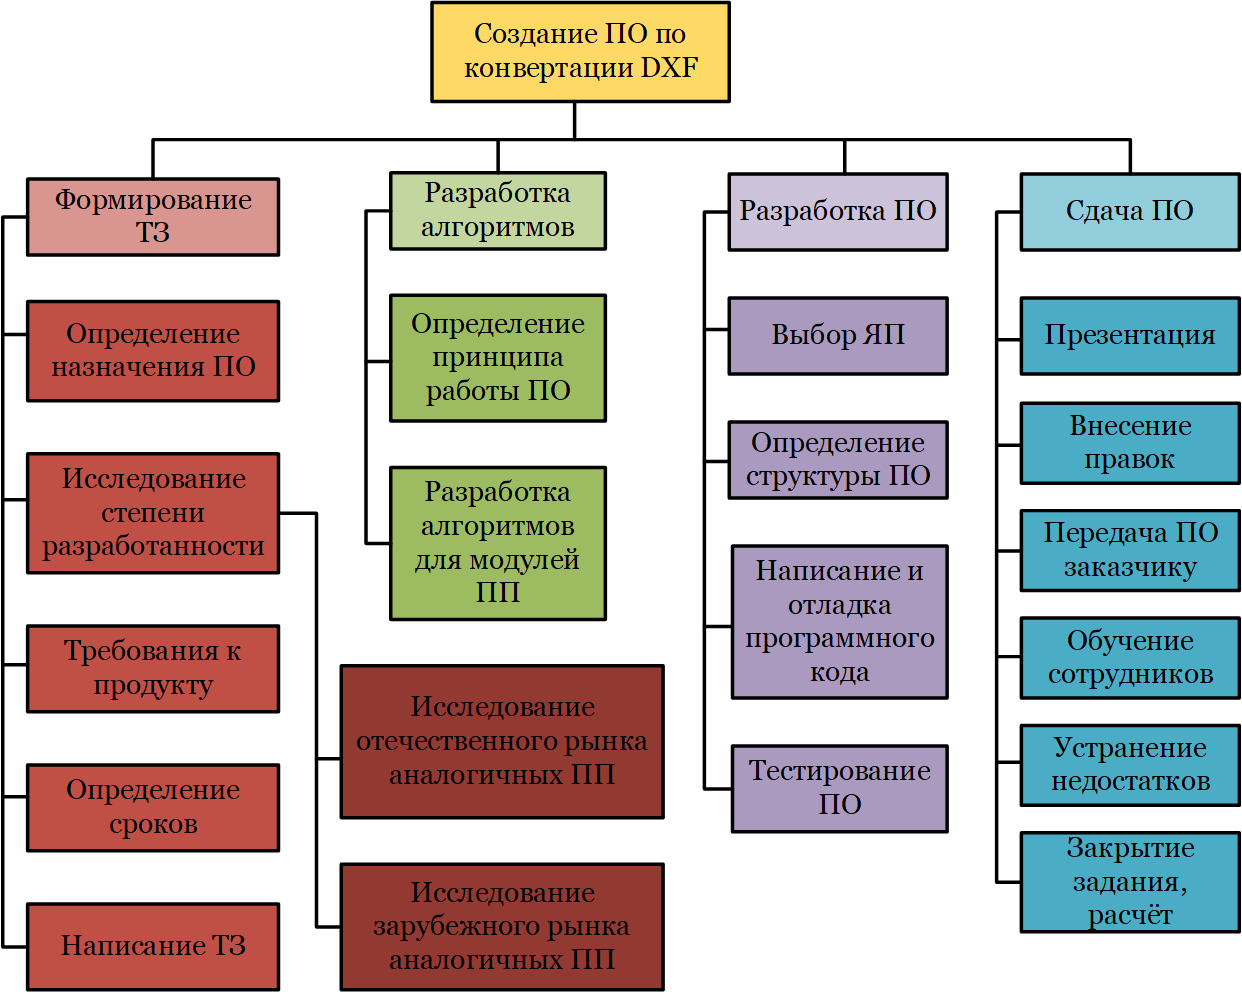
\includegraphics[width=1.0\textwidth]{figures/projektaufgaben.png}
	\captionof{figure}{Дерево задач проекта}
	\label{fig:projektaufgaben}
\end{figure}

\section{Построение диаграмм проекта}

В целях визуализации информации в области планирования проекта, а также для удобства, наглядности и гибкости контроля за выполнением задач проекта используются методы построения диаграмм и графов проекта.

\subsection{Диаграмма Ганта}

На данном этапе строится диаграмма Ганта (англ. Gantt Chart, также, ленточная диаграмма, график Ганта) --- это тип столбчатых диаграмм, использующийся для иллюстрации плана, графика работ проекта. Изобрёл такой тип диаграмм американский <<прародитель>> менеджмента Генри Лоренс Гант \cite{gantt}. Также, является методом планирования проекта. Эта диаграмма представляет собой отрезки (графические плашки), размещающиеся на горизонтальной шкале времени. Каждый отрезок соответствует отдельно задаче (подзадаче). Начало, конец и длина отрезка на шкале времени соответствуют началу, концу и длительности задачи. Диаграмма может использоваться для представления текущего состояния выполнения работ: часть прямоугольника, отвечающего задаче, заштриховывается, отмечая процент выполнения задачи; показывается вертикальная линия, отвечающая моменту «сегодня».

Рядом с самой диаграммой располагается таблица со списком работ, строки которой соответствуют отдельным задачам, отображённым на диаграмме, в то время как столбцы содержат дополнительную информацию о задаче.


%\begin{sidewaysfigure}[H]
%	\centering
%	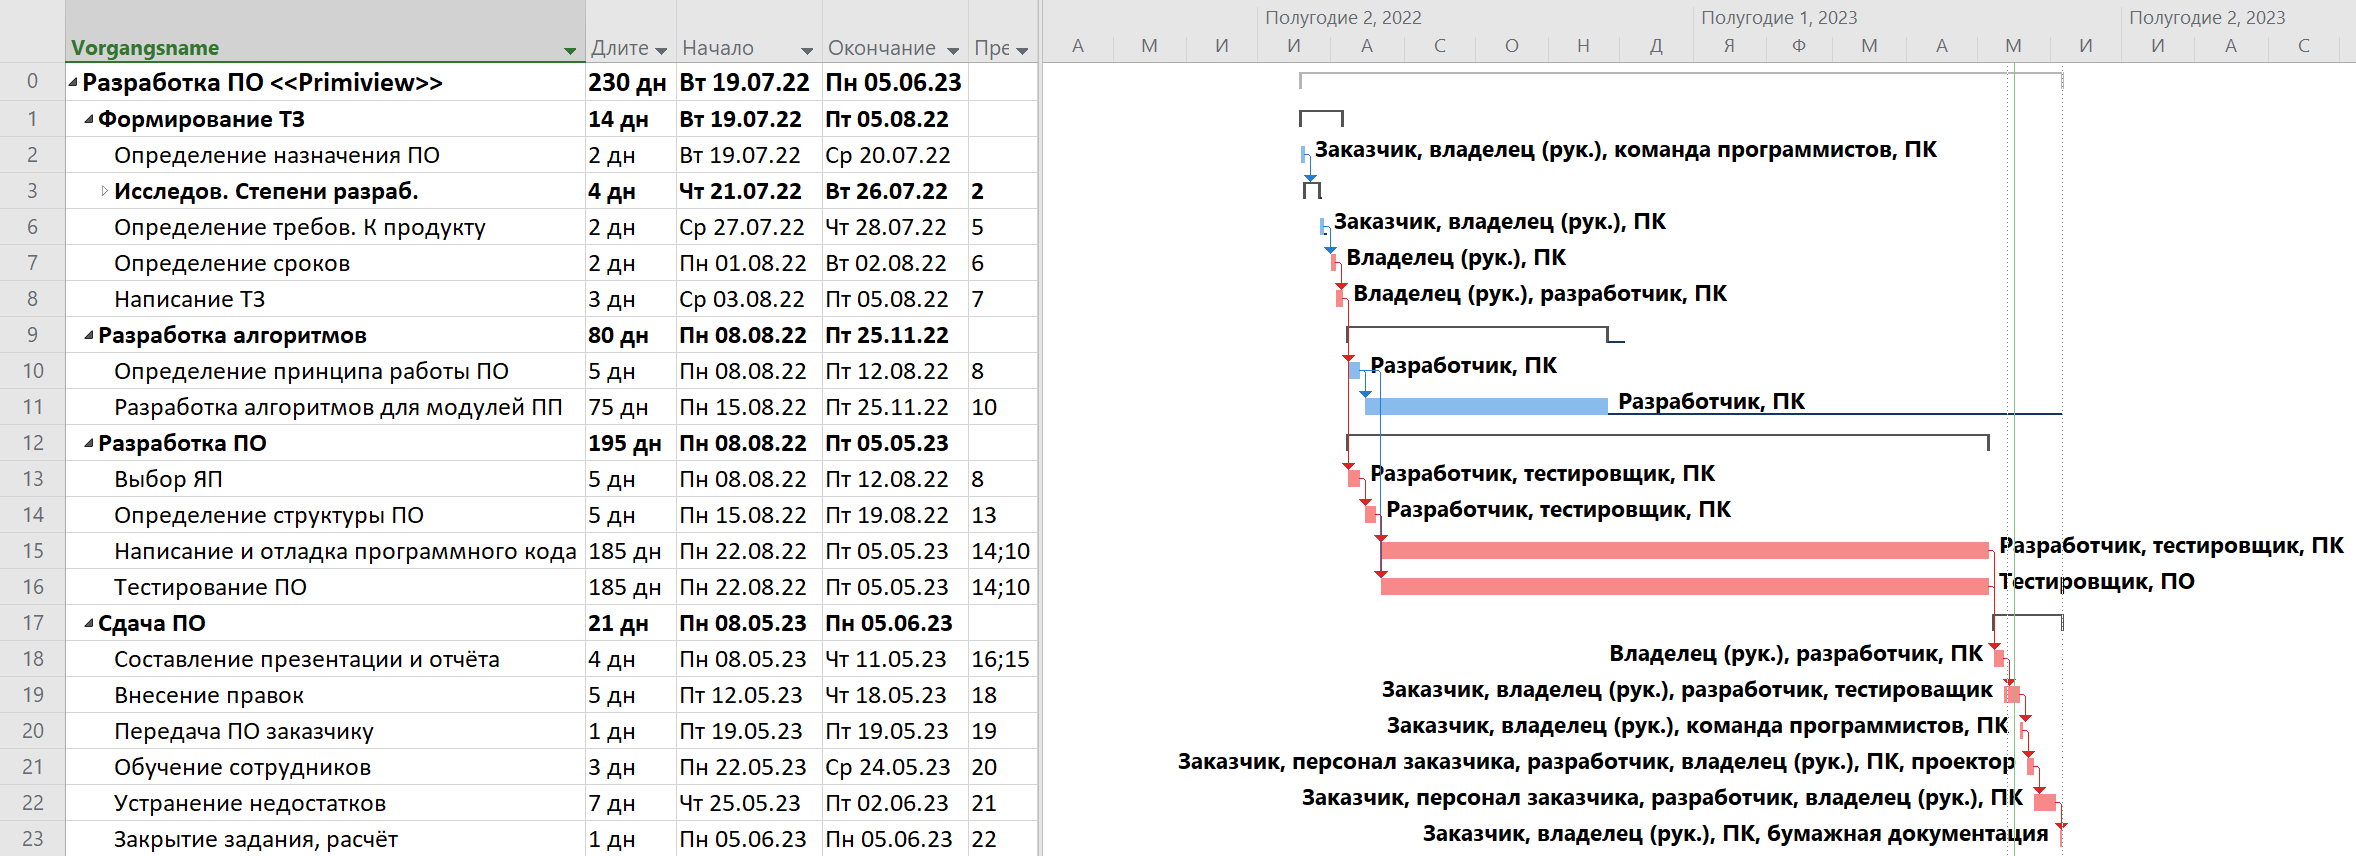
\includegraphics[width=\textwidth, height=0.5\textheight]{figures/gantt.png}
%	\captionof{figure}{Диаграмма Ганта для проекта}
%	\label{fig:gantt}
%\end{sidewaysfigure}


%\begin{landscape}
%\begin{sideways}
%\KOMAoptions{paper=landscape, pagesize}
%\recalctypearea
%\begin{landscape}
\begin{figure}[H]
	\centering
	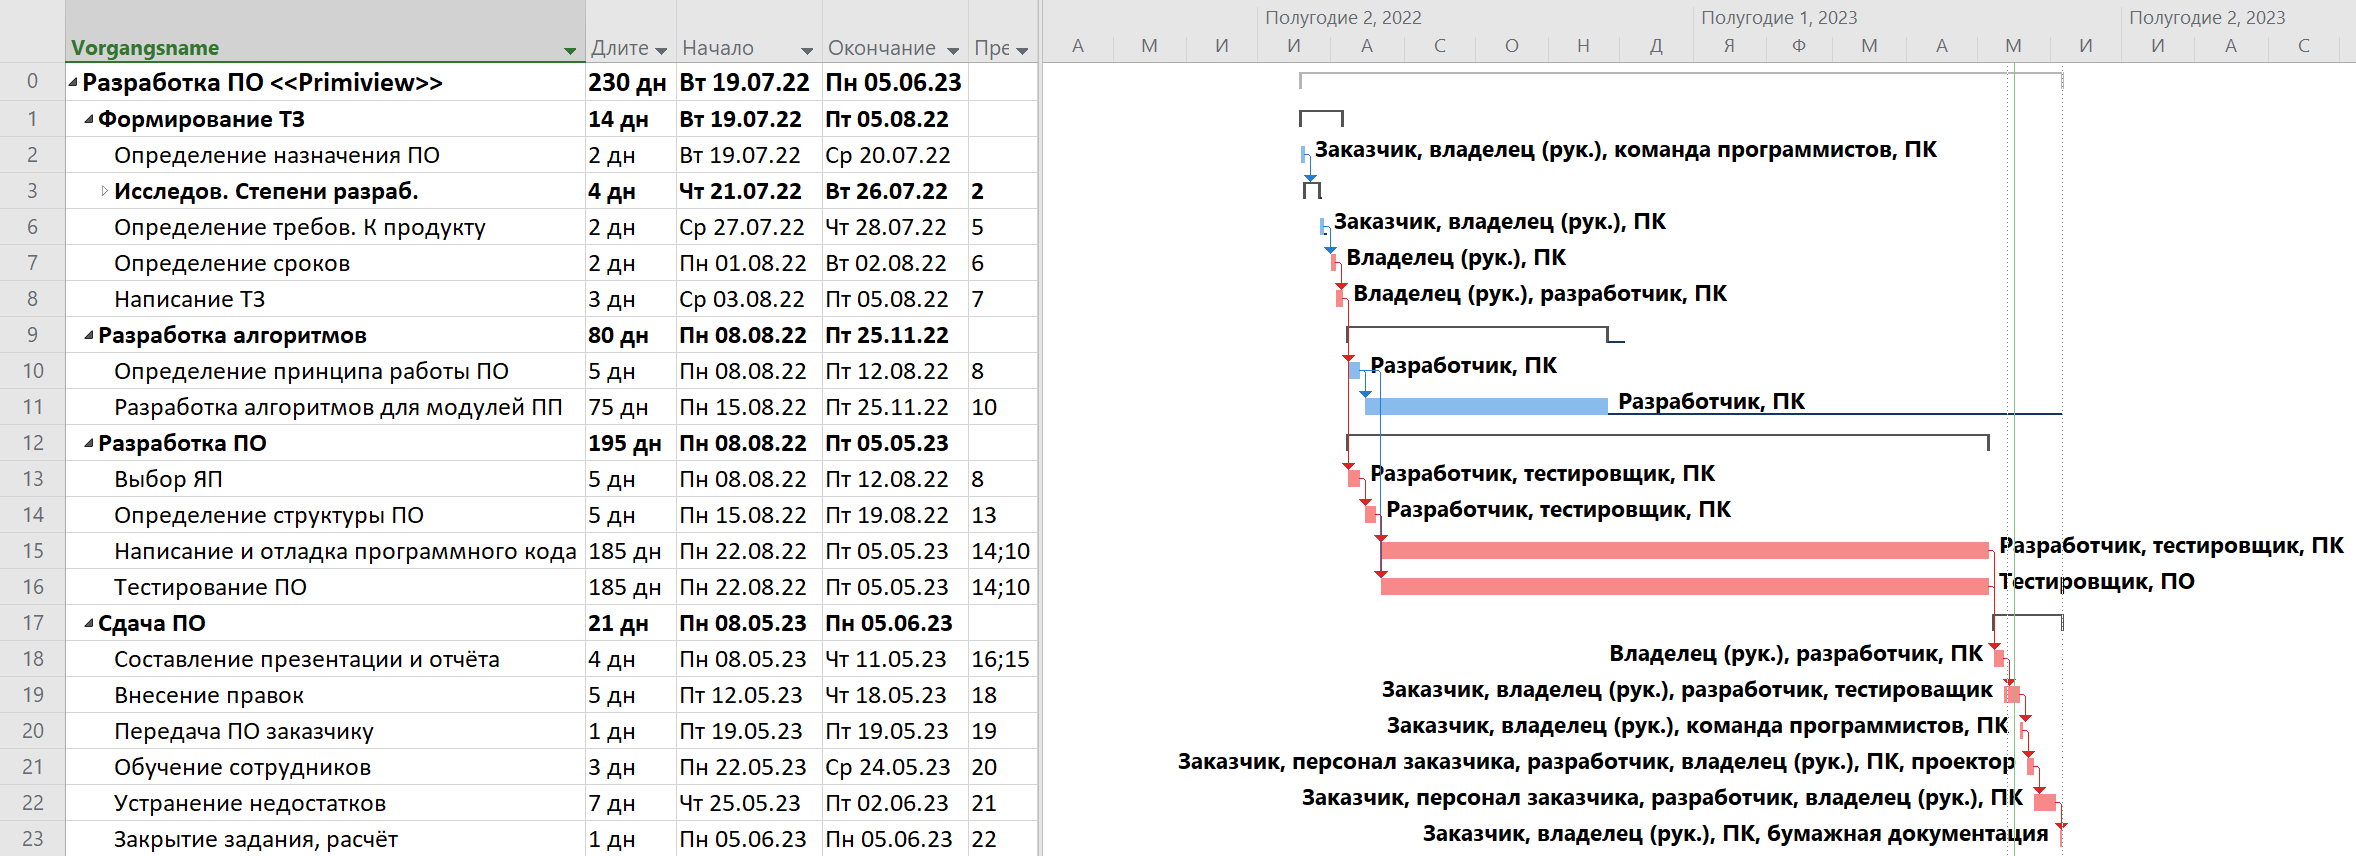
\includegraphics[width=1.4\textwidth, angle=90]{figures/gantt.png}
	\captionof{figure}{Диаграмма Ганта для проекта}
	\label{fig:gantt}
\end{figure}
%\end{landscape}
%\KOMAoptions{paper=portrait, pagesize}
%\recalctypearea
%\end{sideways}
%\end{landscape}

\subsection{Сетевой график}

С целью точного определения плановых сроков завершения проекта и выявления потенциальных вариантов их сокращения, а также для выявления и планирования критического пути проекта строится сетевой график.

Сетевой график представляет собой ориентированный граф, изображающий все необходимые для достижения цели проекта операции в технологической взаимосвязи. Другими словами, это изображение комплекса работ с учётом их длительности, взаимосвязи и перечнем неделимых операций в порядке их выполнения.

Основной элемент сетевого графика --- события, характеризующие завершение или начало работы. Оно обычно обозначается окружностью внутри которой располагается номер события (для сверки со справочной таблицей, прилагающейся к сетевому графику).

Стрелками на сетевом графике изображаются работы --- реальные процессы или действия, требующие затрат труда, материалов и времени, и приводящие к событию, на которое обращена стрелка. Работы на сетевом графике обычно означают одно из следующего:
\begin{itemize}
	\item Действительная работа --- производственный или творческий процесс, требующий усилий, затрат труда, времени и материальных ресурсов;
	\item Ожидание --- процесс, требующий только затрат времени без привлечения каких-либо ресурсов;
	\item Зависимость (фиктивная работы) --- процесс, не требующий затрат труда, времени и ресурсов.
\end{itemize}

Продолжительность работы для проектов на глобальном уровне обычно измеряется, как минимум, днями. Однако на разной масштабности может также и быть оценена в часах, неделях, месяцах, годах. Работы могут иметь количественные показатели, характеризующие трудоёмкость, стоимость, материальные ресурсы.

Временные показатели изображаются над стрелками, обозначение работ --- под стрелками.

К сетевым графикам предъявляется требование, чтобы события были определены полно и чётко, их формулировка должна включать результат предшествующих ему работ. Если то или иное событие наступило, то это значит, что сразу могут быть начаты следующие работы.

Путь на сетевом графике --- это непрерывная последовательность работ от исходного до завершающего события.

Критическим путём называется путь сетевого графика с наибольшей суммарной продолжительностью работ.

При построении сетевых графиков необходимо придерживаться следующих правил:
\begin{enumerate}
	\item Последовательное изображение работ от начала к окончанию,
	\item Изображение стрелок от предшествующего события к последующему,
	\item Отсутствие пересечения стрелок,
	\item Обозначение работ: между двумя событиями только одна стрелка,
	\item Запрет на замкнутые контуры, тупики, хвостовые работы,
	\item Изображение дифференциально-зависимых работ с помощью пунктирных стрелок,
	\item Изображение поставки-результата внешней работы, используемого в данной работе,
	\item Кодирование событий.
\end{enumerate}

Согласно описанным принципам построения сетевых графиков был разработан сетевой график для проекта по разработке ПО <<Primiview>> для конвертирования файлов. На рисунке \ref{fig:netzkompakt} изображена сама сеть. Для расшифровки событий и работ см. таблицы \ref{tab:netzarbeiten} и \ref{tab:netzersch}.

\begin{figure}[H]
	\centering
	\includegraphics[width=\textwidth, angle=0]{figures/netzkompakt.png}
	\captionof{figure}{Сетевой график проекта}
	\label{fig:netzkompakt}
\end{figure}

\begin{longtable}{|m{0.06\textwidth}|p{0.57\textwidth}|m{0.08\textwidth}|m{0.10\textwidth}|}
	\caption{Работы в сетевом графике проекта}
	\label{tab:netzarbeiten}
	\centering
	\tabularnewline
	\hline
	\multicolumn{1}{|m{0.10\textwidth}|}{Обозн.}&\multicolumn{1}{c|}{Наименование этапа}&\multicolumn{1}{m{0.12\textwidth}|}{Продолж.\newline (раб. дней)}&\multicolumn{1}{m{0.10\textwidth}|}{Предш. этап}\\
	\hline \endfirsthead
	\subcaption{Продолжение таблицы~\ref{tab:netzarbeiten}}\\
	\hline \endhead
	\subcaption{Продолжение на след. стр.}
	\endfoot
	%\hline
	\endlastfoot
	A&Принятие командой проекта решений по назначению ПО, исследование аналогов, определение требований и сроков&14&-\\ \hline
	B&Определение файловых потоков&2&A\\ \hline
	C&Определение взаимосвязи файлов ПО&3&B\\ \hline
	D&Сравнение концепций хранения данных внутри ПО, схематизация и моделирование вариантов реализации алгоритма, проверка алгоритма на ошибки&10&C\\ \hline
	E&Вывод зависимостей между доступными параметрами дуг и необходимой геометрией дуг, разработка алгоритма&10&C\\ \hline
	F&Разработка алгоритма по перебору и внутрепрограммному сохранению координат изображения&10&C\\ \hline
	G&Разработка алгоритма на основе созданной структуры хранения примитивов&10&D\\ \hline
	H&Разработка алгоритма с использованием созданных алгоритмов вычленения необходимой информации из DXF-файлов&10&E\\ \hline
	I&Применение встроенных в ЯП методов сортировки, применение предыдущего алгоритма&2&F\\ \hline
	J&Выполнение операций над краевыми значениями массивов координат&1&F\\ \hline
	K&Разработка алгоритма конвертации с использованием радиуса сегмента полилиний&5&G,H\\ \hline
	L&Разработка алгоритма конвертации с использованием альтернативного метода описания дуг&10&J\\ \hline
	M&Разработка алгоритма с использованием встроенных в ЯП алгоритмов сортировки&2&I\\ \hline
	N&Разработка алгоритма с использованием извлечённых из DXF Геометрических данным для визуализации изображения&5&H,K\\ \hline
	O&Разработка алгоритма конвертации DXF В JSON с объединением примитивов в контуры&10&L,M,N\\ \hline
	P&Сравнительный анализ ЯП в применении к поставленным требованиям к ПО&5&O\\ \hline
	Q&Написание кода программы и его отладка&138&P\\ \hline
	R&Тестирование функционала разработанного ПО&138&Q\\ \hline
	S&Подготовка документа-отчёта, а также составление презентации с подготовкой команды проекта к демонстрации разработанного ПП&4&R\\ \hline
	T&Подготовка презентации и отчёта с незавершёнными тестами ПО&2&Q\\ \hline
	U&Заслушивание обратной связи заказчика после презентации. Составление списка замечаний к исправлению&6&S,T\\ \hline
	V&Проведение обучения сотрудников заказчика к пользованию ПП. Передача ПО заказчику. Предоставление времени на внутреннюю проверку нового ПО&10&U\\ \hline
	W&Приём списка замечаний сотрудников заказчика после периода внутренней апробации ПП&7&V\\ \hline
	X&Обновление переданного ПО заказчику. Завершающая встреча заказчика и владельца проекта для подписания оформленных к завершению проекта документов&1&W\\ \hline
\end{longtable}

\begin{longtable}{|m{0.06\textwidth}|p{0.70\textwidth}|m{0.10\textwidth}|}
	\caption{События в сетевом графике проекта}
	\label{tab:netzersch}
	\centering
	\tabularnewline
	\hline
	\multicolumn{1}{|m{0.10\textwidth}|}{Обозн.}&\multicolumn{1}{c|}{Наименование события}&\multicolumn{1}{m{0.12\textwidth}|}{Предш. событие}\\
	\hline \endfirsthead
	\subcaption{Продолжение таблицы~\ref{tab:netzersch}}\\
	\hline \endhead
	\subcaption{Продолжение на след. стр.}
	\endfoot
	%\hline
	\endlastfoot
	1&Начало проекта&-\\ \hline
	2&Техническое задание&1\\ \hline
	3&Схема работы ПО&2\\ \hline
	4&Структура ПО&3\\ \hline
	5&Алгоритм внутрепрограммного сохранения примитивов&4\\ \hline
	6&Алгоритм вычисления радиуса сегмента полилинии&4\\ \hline
	7&Алгоритм вычленения координат из объектов DXF&4\\ \hline
	8&Алгоритм конвертации DXF$\rightarrow$TXT(DXF-type)&5\\ \hline
	9&Алгоритм поиска наименьших координат изображения&7\\ \hline
	10&Алгоритм поиска ширины и высоты рамки объектов DXF&7\\ \hline
	11&Алгоритм конвертации DXF$\rightarrow$TXT(x,y,r)&6,8\\ \hline
	12&Алгоритм конвертации DXF$\rightarrow$SVG&9,10,11\\ \hline
	13&Алгоритм конвертации DXF$\rightarrow$JSON&12\\ \hline
	14&Утверждённый руководителем проекта ЯП&13\\ \hline
	15&Файлы проекта с исходным кодом&14\\ \hline
	16&Отчёт о прохождении тестов&15\\ \hline
	17&Презентация и отчёт проекта в эл.виде&16\\ \hline
	18&Список правок&17\\ \hline
	19&Результаты тестирования сотрудников&18\\ \hline
	20&Список устранённых недостатков&19\\ \hline
	21&Подписанное о закрытии задание проекта. Счёт на оплату. Чек об оплате&20\\ \hline
\end{longtable}


%\section{Расчёт стоимости проекта}
%
%Ресурс — средства, позволяющие с помощью определённых преобразований получить желаемый результат. 
%
%После того как определен состав задач, необходимо определить, кто эти задачи будет исполнять и какое оборудование будет использоваться. Для этого нужно ввести в план проекта список ресурсов и информацию о них, а затем распределить эти ресурсы между задачами. 
%
%С задачами, для которых назначены сроки, должны быть ассоциировано оборудование, средства и люди. Это подразумевает распределение обязанностей. Эта деятельность определяется и ограничивается доступностью ресурсов, их оптимальным использованием в заданном контексте и вопросами, связанными с персоналом.  
%
%Для того чтобы определить стоимость всего проекта, необходимо обозначить виды ресурсов, стоимость этих ресурсов, время использования и необходимый объем.  












\section{Сравнительная экономическая эффективность}

Расчеты сравнительной экономической эффективности капитальных вложений (инвестиций) применяются при сопоставлении нескольких возможных для осуществления вариантов инженерных решений: при решении задач по выбору взаимозаменяемых материалов, внедрению новых видов техники, модернизации оборудования, способов организации производственных процессов и т. п. То есть для оценки решений, которые являются альтернативными для обеспечения одинаковых конечных результатов деятельности. При этом конечные результаты (производство конкретной продукции с определенными характеристиками в заданном объеме) уже известны, есть необходимость определить, какой способ ее изготовления на том или ином этапе деятельности предприятия является более выгодным.

\subsection{Исходные данные}

Станкостроительное предприятие рассматривает заказ на создание программного обеспечения для своего оборудования (токарных станков с ЧПУ). Это ПО автоматизирует процесс создания управляющих программ для станков с ЧПУ, взамен работе инженера-технолога-программиста, который, обычно, берёт чертёж детали и либо вручную пишет УП, либо использует иностранные CAM-системы, предварительно создавая 3d-модель по выданному чертежу.
В рамках данной (третьей) части ВКР будет рассматриваться инвестиционный проект (ИП) с точки зрения покупателя оборудования у предприятия, которое привлекло силы университета для создания описанного ПО. Сравниваются два варианта – покупка станков без ПО и, соответственно, с ним.

\paragraph{Сравнительная характеристика вариантов.} Рассмотрим ситуацию с точки зрения покупателя оборудования рассматриваемого станкостроительного предприятия. Соберём основные данные в таблицу  \ref{tab:startcomparis}.

\begin{longtable}{|p{0.50\textwidth}|p{0.50\textwidth}|}%{|p{0.40\textwidth}|c|}
	\caption{Сравнительная характеристика вариантов ИП}
	\label{tab:startcomparis}
	\centering
	\tabularnewline
	\hline
	Вариант 1      & Вариант 2\\
	\hline \endfirsthead
	\subcaption{Продолжение таблицы~\ref{tab:startcomparis}}\\
	\hline \endhead
	\subcaption{Продолжение на след. стр.}
	\endfoot
	%\hline
	\endlastfoot
	Покупка станка без ПО	&	Покупка станка вместе с ПО (CAM-системой) за большую цену\\
	\hline
	Наём во время этапа подготовки производства инженеров-технологов-программистов для написания УП	&	Привлекаются технологи из имеющегося штата сотрудников для выполнения дополнительных обязанностей по контролю создания УП с помощью купленного ПО\\
	\hline
	Время написания УП в три раза дольше, чем во втором варианте	&	Время написания УП в течение одного часа (в среднем)\\
	\hline
\end{longtable}

Варианты рассматриваются с точки зрения потребителя оборудования.
За сопоставляемые характеристики принимаются следующие:

\begin{itemize}
	\item Объём производства (серийное),
	\item Частота создания УП в год (200 новых УП в среднем).
\end{itemize}

\paragraph{Выбор единичного периода времени.} В качестве единичного периода времени для расчётов примем один год, так как на рассматриваемом предприятии-клиенте ситуация с производством каждый месяц практически не меняется. Также, большинство справочных величин ссылаются именно на годовой период, что тоже является подтверждением равномерной распределённости экономических характеристик внутри отдельно взятых месяцев.

\paragraph{Состав и описание капитальных вложений по вариантам.} В капитальные вложения входят следующие величины:

\begin{itemize}
	\item Цена станка с без ПО – 2 750 000 руб.,
	\item Цена встроенной CAM-системы на единицу оборудования– 70 000 руб.,
	\item Наладка полной группы станков – 20 000 руб.
\end{itemize}

\paragraph{Принятие решения по нормативному сроку окупаемости и его обоснование.} Соответствует требованиям к сроку окупаемости дополнительных капитальных вложений, в данном случае – в токарный станок с ЧПУ.

Срок полезного использования оборудования – 10 лет.

Срок контракта на выпуск продукции с использованием данного оборудования – в рассматриваемой ситуации нет ограничений, токарная обработка постоянно проводится на предприятии.

Требования собственника, инвестора – предприятие установило желаемый срок окупаемости – 5 лет.

Следовательно, задаём Тн (нормативный срок окупаемости) равным 5 лет, так как временные рамки требований инвестора меньше срока полезного использования оборудования.

\paragraph{Определение состава затрат по вариантам (результат – перечень затрат).} Корректировка затрат в соответствии с возможностями Методики сравнительной эффективности (включаем в расчет только различающиеся по альтернативам затраты). Деление затрат на переменные и постоянные. Формирование списка исходных данных для выполнения расчетов (см. таблицу \ref{tab:gegeben}).

\begin{longtable}{|p{0.30\textwidth}|p{0.30\textwidth}|p{0.30\textwidth}|}
	\caption{Исходные данные для расчётов текущих затрат}
	\label{tab:gegeben}
	\centering
	\tabularnewline
	\hline
 	\quad & \multicolumn{1}{c|}{Вариант 1} & \multicolumn{1}{c|}{Вариант 2}\\
	\hline \endfirsthead
	\subcaption{Продолжение таблицы~\ref{tab:gegeben}}
	\\ \hline \endhead
	\subcaption{Продолжение на след. стр.}
	\endfoot
	%\hline
	\endlastfoot
	\multicolumn{3}{|c|}{Переменные затраты (на единицу объема деятельности (одну УП))}\\
	\hline
	Зарплата технолога, руб & \multicolumn{1}{c|}{1500} & \multicolumn{1}{c|}{1500}\\
	\hline
	Время на написание одной УП, час & \multicolumn{1}{c|}{3} & \multicolumn{1}{c|}{1}\\
	\hline
	\multicolumn{3}{|c|}{Постоянные затраты (на единицу оборудования)}\\
	\hline
	Цена годовой лицензии/контракта обслуживания CAM-системы, руб & \multicolumn{1}{c|}{50000} & \multicolumn{1}{c|}{55000}\\
	\hline
\end{longtable}

\subsection{Расчёты и анализ}

Так как выбран нормативный срок окупаемости, равный одному году, то к нему будут приведены расчёты по приведённым затратам.

\paragraph{Исходные данные.}

\nopagebreak

Среднее годовое количество УП на предприятии-покупателе станков
\[N=200 \text{ шт;}\]

Срок полезного использования оборудования:
\[T_{machinery}=10 \text{ лет;}\]

Требования инвестора по окупаемости ИП:
\[T_{inv}=5 \text{ лет;}\]

Принятая норма окупаемости:
\[{T_n=T}_{inv}=5 \text{ лет;}\]

Наладка полной группы станков:
\[{CAM}_{Term}=20000 \text{ руб;}\]

Цена встроенной CAM-системы на единицу оборудования:
\[{CAM}_2=70000 \text{ руб;}\]

Цена станка без встроенной CAM-системы:
\[M=2750000 \text{ руб;}\]

Цена годовой лицензии/контракта обслуживания CAM-системы на единицу оборудования для вариантов 1 и 2, соответственно:
\[{CAM}_{1Perm}=50000 \text{ руб;}\]

\[{CAM}_{2Perm}=55000 \text{ руб;}\]

Среднее время написания одной УП:
\[t_1=3 \text{ часа;}\]
\[t_2=1 \text{ час;}\]

Почасовая оплата технолога:
\[Sal=1500 \text{ руб;}\]

Страховые сбора от заработной платы:
\[fees=30\%\]

Количество покупаемых станков:
\[N_M=5 \text{ шт;}\]

\paragraph{Расчёт.}\label{par:ecocalc}

Себестоимость использования оборудования и ПО:
\begin{equation}
	\begin{aligned}
		C_1 = Sal \cdot t_1\cdot N \cdot(100\%+fees)+N_M \cdot CAM_{1Perm} =\\= 1500 \cdot 3 \cdot 200 \cdot (100\%+30\%)+5 \cdot 50000=1 420 000 \text{ руб;}
	\end{aligned}
\end{equation}
\begin{equation}
	\begin{aligned}
		C_2 = Sal \cdot t_2\cdot N \cdot(100\%+fees)+N_M \cdot CAM_{2Perm} =\\= 1500 \cdot 1 \cdot 200 \cdot (100\%+30\%)+5 \cdot 55000=665 000 \text{ руб;}
	\end{aligned}
\end{equation}

Условно-годовая экономия (на себестоимости):
\begin{equation}
	\begin{aligned}
		E=|C_1-C_2|=|1420000-665000|=755 000 \text{ руб;}
	\end{aligned}
\end{equation}

Капитальные вложения предприятия-покупателя станков:
\begin{equation}
	\begin{aligned}
		K_1=M \cdot N_M+{CAM}_{Term}=2750000 \cdot 5+20000=13 770 000 \text{ руб;}
	\end{aligned}
\end{equation}
\begin{equation}
	\begin{aligned}
		K_2=N_M \cdot (M+{CAM}_2)+{CAM}_{Term}=\\=5 \cdot (2750000+70000)+20000 = 14 120 000 \text{ руб;}
	\end{aligned}
\end{equation}

Дополнительные капитальные вложения:
\begin{equation}
	\begin{aligned}
		K_{extr}=|K_1-K_2|=|13770000-14120000|=350 000 \text{ руб;}
	\end{aligned}
\end{equation}
\begin{equation}
	\begin{aligned}
		K_{extr}=N_M \cdot {CAM}_2=5 \cdot 70000=350 000 \text{ руб. (проверка);}
	\end{aligned}
\end{equation}

Срок окупаемости дополнительных капитальных вложений:
\begin{equation}
	\begin{aligned}
		T_{payback}=\frac{K_{extr}}{E}=\frac{350000}{755000}=0,464 \text{ лет;}
	\end{aligned}
\end{equation}

Приведённые затраты по вариантам:
\begin{equation}
	\begin{aligned}
		Z_1=C_1+\frac{1}{T_n} \cdot K_1=1420000+\frac{1}{5} \cdot 13770000=4 174 000 \text{ руб;}
	\end{aligned}
	\label{F:spends1}
\end{equation}
\begin{equation}
	\begin{aligned}
		Z_2=C_2+\frac{1}{T_n} \cdot K_2=665000+\frac{1}{5} \cdot 14120000=3489000 \text{ руб;}
	\end{aligned}
	\label{F:spends2}
\end{equation}

Годовой экономический эффект:
\begin{equation}
	\begin{aligned}
		E_{annual}=|Z_1-Z_2|=|4174000-34890000|=685000 \text{ руб;}
	\end{aligned}
\end{equation}

Минимальный годовой объём деятельности, при котором обеспечивается приведённый годовой экономический эффект:
\begin{equation}
	\begin{aligned}
		N_{cr}=\frac{N_M \cdot CAM_{1Perm}-N_M \cdot CAM_{2Perm}-\frac{K_{extr}}{T_n}}{S \cdot t_2 \cdot (100\%+fees)-Sal \cdot t_1 \cdot (100\%+fees)}=\\=\frac{5 \cdot 50000-5 \cdot 55000-\frac{350000}{5}}{1500 \cdot 1 \cdot 100\%+30\%-1500 \cdot 3 \cdot 100\%+30\%}=24,359 \text{ шт;}
	\end{aligned}
\end{equation}

По вычисленным в формулах \ref{F:spends1}, \ref{F:spends2} затратам изобразим на графике (см. рисунок \ref{fig:economyborders}) границы целесообразности рассматриваемых вариантов.

\pgfplotsset{width=13cm,compat=1.9}
\begin{figure}[H]
	\centering
	\begin{tikzpicture}
		\centering
		\begin{axis}[ 
			xlabel = {$N, \text{шт. (объём деятельности)}$},
			ylabel = {$Z, \text{руб. (приведённые затраты)}$},
			xmin=0, xmax=200, ymin=2900000,
			xtick={0,20,40,60,80,100,120,140,160,180,200},
			ymajorgrids=true,
			xmajorgrids=true
			]
			\addplot[line width=1mm,  blue, mark=*] coordinates {
				(0,3004000) (200,4174000)
			};
			\addplot[line width=1mm,  red, mark=triangle] coordinates {
				(0,3099000) (200,3489000)
			};
%			\node at (axis cs:0,4200000) [anchor = north west] {\text{Границы целесообразности}};
		\end{axis}
		\label{graph:economyborders}
	\end{tikzpicture}
	\captionof{figure}{Границы целесообразности рассматриваемых вариантов}
	\label{fig:economyborders}
\end{figure}

Получив необходимые значения по критериям сравнения, сведём результаты в таблицу \ref{tab:fintabeco}).

%\begin{longtable}{|p{0.40\textwidth}|p{0.05\textwidth}|p{0.15\textwidth}|p{0.15\textwidth}|p{0.15\textwidth}|}
\begin{longtable}{|p{0.40\textwidth}|p{0.05\textwidth}|p{0.13\textwidth}|p{0.13\textwidth}|p{0.13\textwidth}|}
	\caption{Сравнительная характеристика рассматриваемых вариантов по показателям эффективности}
	\label{tab:fintabeco}
	\centering
	\tabularnewline
	\hline
	\multicolumn{1}{|c|}{\multirow{3}{6cm}{Наименование показателя}} & \multicolumn{1}{c|}{\multirow{3}{1cm}{Ед. изм.}} & \multicolumn{2}{c|}{По вариантам:} & \multicolumn{1}{c|}{\multirow{3}{3cm}{Отклонения показателей}}\\
	\cline{3-4} 
	\endfirsthead
	\subcaption{Продолжение таблицы~\ref{tab:fintabeco}}
	\\ \hline \endhead
	\subcaption{Продолжение на след. стр.}
	\endfoot
	%\hline
	\endlastfoot
	\multicolumn{1}{|c|}{}&\multicolumn{1}{c|}{}&Вариант без ПО&Вариант c ПО&\multicolumn{1}{c|}{}\\
	\hline
	Годовой объем деятельности&шт.&200&200&-\\
	\hline
	Капитальные вложения, всего&руб.&13770000&14120000&350000\\
	\hline
	\multicolumn{5}{|l|}{в том числе:}\\
	\hline
	Наладка станков&руб.&20000&20000&-\\
	\hline
	Цена станка (Вар. 2 + ПО)&руб.&13750000&665000&755000\\
	\hline
	Срок окупаемости дополнительных кап. вложений&&0,464&&\\
	\hline
	Приведённые затраты по вариантам&руб.&4174000&3489000&658000\\
	\hline
	Годовой экономический эффект&&&685000&\\
	\hline
\end{longtable}


\subsection{Выводы по результатам расчётов.}

Так как на первых этапах расчёта по методу сравнительной эффективности ИП нельзя было сделать конкретный вывод по поводу целесообразности одного из предлагаемых вариантов по причине того, что по первому варианту себестоимость ИП была больше в сравнении со вторым, а капитальные вложения, соответственно, меньше, то расчёт был продолжен до момента вычисления расчётного срока окупаемости дополнительных капитальных вложений, а также расчёта приведённых затрат по каждому из вариантов.

Исходя из расчётов и построенного по ним графика, сделаем вывод, что, производя уже 25 УП за год, выгоднее становится вариант с ПО, так как приведённые затраты для соответствующего количество производимых УП для этого варианта оказываются меньше.

Анализируя итоговые данные, выбираем для реализации второй вариант, то есть покупка оборудования вместе со встроенным ПО (CAM-системой), объясняя выбор тем, что расчётный срок окупаемости оказался намного меньше рассматриваемого нормативного срока окупаемости (0,4 и 5 лет, соответственно), а приведённые затраты по первому варианту оказались больше, чем по второму.

Действительно, экономия времени на создании УП нивелирует большие капитальные вложения на этапе инвестиционного периода УП.

\section{Выводы по главе \ref{cha:wirtsch}}

\begin{enumerate}[1)]
	\item Разработана экономическая модель проекта;
	\item Построено дерево задач, необходимых для выполнения целей проекта. На верхнем уровне иерархии получилось 4 задачи: формирование ТЗ, разработка алгоритмов, разработка ПО и сдача ПО;
	\item Построена диаграмма Ганта и сетевой график,  в результате которых проект спланирован для реализации за 230 календарных дней. Наименьшая длительность проекта: 223 дня;
	\item Проведён анализ сравнительной экономической эффективности проекта. Было установлено, что при производстве 25 УП в год с помощью разработанного ПО, приведённые затраты по варианту с внедрением этого ПО становятся меньше по сравнению с вариантом без него. Из этого следует выгодность внедрения приложения при заданных условиях.
\end{enumerate}

%%% Local Variables:
%%% mode: latex
%%% TeX-master: "rpz"
%%% End:


%\chapter{Определение области применения и главных требований к разрабатываемым конвертерам}
\label{cha:analysis}
%
% % В начале раздела  можно напомнить его цель
%
В данном разделе поясняется область применения разрабатываемого ПО, а также, указываются требования к разрабатываемым конвертерам.

\section{Область применения ПО <<Primiview>>}

Конвертер в TXT по типу DXF применяется для контроля содержания необходимых (поддерживаемых) примитивов (объектов) в DXF-файле. Также, с помощью данного формата может производится расчёт длины траектории  контура детали (обычно, в поперечном её сечении). Это может быть полезно при применении ПО в области лазерной резки с помощью станков с ЧПУ, а, в частности, в ПО <<Сириус>>.

Конвертер из DXF в TXT в формате координат и радиуса применяется для автоматизированного технологического проектирования, для формирования УП. Получаемая в результате работы ПО информация о примитивах изображения контура детали используется для непосредственного составления УП, так как каждая последующая точка имеет не только плоские координаты, но и способ достижения этой точки (тип примитива: отрезок, если радиус равен нулю; дуга, если радиус ненулевой).

Конвертер в SVG-формат полезен для последующего формирования других типов файлов (например, DBS), а также, для компактного по объёму файла векторного представления контура детали. ИВЗУАЛИЗАЦИЯ. ПОДробно о svg - литературный обзор. Внутренняя репрезентация (ezdxf)

Конвертер в JSON удобен для хранения информации об объектах контура детали. В этом формате работает и другое ПО разрабатываемой САПР для формирования УП для станков с ЧПУ.

В целом, разрабатываемый набор конвертеров (модуль экспорта) представляет собой цельный ПП, сочетающий в себе набор необходимых разработчику УП начальных функций для автоматизированного технологического проектирования. Это ПО может быть интегрировано в разные ПП, так как по сути универсально в своём применении (используется в области 2D-резки, токарной обработке).



\section{Главные требования ко входному файлу}

Так как данная работа нацелена на создание ПО для обработки геометрической информации 2D-объектов специального типа, то конвертироваться из DXF-файлов должна не вся информация, содержащаяся в них. В первую очередь, заказчиком работы было определено, что на входе будет подаваться 2D-контур деталей типа <<Втулка>>, то есть тел вращения. Так как сконвертированная геометрия данных объектов в последующем предполагает разработку УП для токарных станков с ЧПУ, то геометрическая информация должна содержать определённый набор геометрических примитивов, с которым может работать система исполнительных органов станков с ЧПУ. Этот набор ограничивается тем, что исполнительные органы станков с ЧПУ способны перемещаться либо с помощью \textbf{линейной}, либо с помощью \textbf{круговой интерполяции}. Из этого следует, что для корректной работы САПР, для которых предназначаются разрабатываемые конвертеры, геометрия в DXF-файле на входе конвертеров должна состоять из, как минимум одного из представленных далее примитивов:

\begin{enumerate}
	\item линия (отрезок),
	\item полилиния,
	\item дуга,
	\item окружность.
\end{enumerate}

Остальные типы геометрии, реализуемой в формате DXF, такие как \textit{эллипс}, \textit{сплайн}, будут игнорироваться ПО.

\section{Описание формата DXF-файлов}\label{sec:allaboutdxf}

На вход разрабатываемому конвертеру подаётся файл формата DXF. Формат DXF представляет собой совокупность данных с тегами всей информации, содержащейся в файле чертежа AutoCAD. Тегированные данные означают, что каждому элементу данных в файле предшествует целое число, называемое групповым кодом. Значение группового кода указывает, какой тип данных имеет следующий элемент. Это значение также указывает смысл элемента данных для данного типа объекта. Практически вся указанная пользователем информация в файле чертежа может быть представлена в формате DXF \cite{Autodesk}.
В DXF файлах, в зависимости от их содержания, существуют сущности, представляющие для нас интерес. Среди них следующие:

\begin{enumerate}
	\item LINE (Линия),
	\item LWPOLYLINE (Полилиния),
	\item ARC (Дуга),
	\item CIRCLE (Окружность),
	\item INSERT (Вставка).
\end{enumerate}

Как уже и было отмечено, существуют и другие примитивы (ELLIPSE, SPLINE и др.), однако, основываясь на конкретных целях заказчика по возможности применения выходных файлов для генерации УП, ПП проектируется только с указанными примитивами и сущностями DXF.

Рассмотрим каждую из сущностей подробнее.

\paragraph{LINE.} Рассмотрим тэги сущности \textit{Линия}, необходимые для её реального отображения (см. табл. \ref{tab:line}).


\begin{longtable}{|l|l|}
	\caption{Рассматриваемые групповые коды сущности LINE}
	\label{tab:line}
	\centering
	\tabularnewline
	\hline
	Групповой код & Описание\\
	\hline \endfirsthead
	\subcaption{Продолжение таблицы~\ref{tab:line}}
	\\ \endhead
	\subcaption{Продолжение на след. стр.}
	\endfoot
	%\hline
	\endlastfoot
	39	&	Толщина (необязательный; по умолч. = 0)\\ \hline
	10	&	Начальная точка (в с.к. объекта) DXF: значение X\\ \hline
	20, 30	&	DXF: Y и Z значения начальной точки (в с.к. объекта)\\ \hline
	11	&	Конечная точка (в с.к. объекта)	DXF: значение X\\ \hline
	21, 31	&	DXF: Y и Z значения конечной точки (в с.к. объекта)\\ \hline
\end{longtable}

\paragraph{LWPOLYLINE.} Рассмотрим тэги сущности \textit{Полилиния}, необходимые для её реального отображения (см. табл. \ref{tab:polyline}).

\begin{longtable}{|p{70pt}|p{370pt}|}
	\caption{Рассматриваемые групповые коды сущности POLYLINE}
	\label{tab:polyline}
	\centering
	\tabularnewline
	\hline
	Групповой код & Описание\\
	\hline \endfirsthead
	\subcaption{Продолжение таблицы~\ref{tab:polyline}}
	\\ \endhead
	\subcaption{Продолжение на след. стр.}
	\endfoot
	%\hline
	\endlastfoot
	70	&	«Флаг» полилинии (бит-закодировано); по умолч. = 0; 1 – закрыта\\ \hline
	39	&	Толщина (необязательный; по умолч. = 0)\\ \hline
	10	&	Координаты вершин (в с.к. объекта), множественные вхождения; по одному вхождению для каждой вершины DXF: значение X\\ \hline
	20	&	DXF: значение Y координат вершин (в с.к. объекта), множественные вхождения; по одному вхождению для каждой вершины\\ \hline
	42	&	\textit{Bulge}. Выпуклость (множественные вхождения - для каждой вершины), (необязательно; по умолч. =0)\\ \hline	
\end{longtable}

\paragraph{ARC.} Рассмотрим тэги сущности \textit{Дуга}, необходимые для её реального отображения (см. табл. \ref{tab:arc}).

\begin{longtable}{|p{70pt}|p{370pt}|}
	\caption{Рассматриваемые групповые коды сущности ARC}
	\label{tab:arc}
	\centering
	\tabularnewline
	\hline
	Групповой код & Описание\\
	\hline \endfirsthead
	\subcaption{Продолжение таблицы~\ref{tab:arc}}
	\\ \endhead
	\subcaption{Продолжение на след. стр.}
	\endfoot
	%\hline
	\endlastfoot
	39	&	Толщина (необязательный; по умолч. = 0)\\ \hline	
	10	&	Центр дуги (в с.к. объекта)
	DXF: значение X\\ \hline	
	20, 30	&	DXF: Y и Z значения центра дуги (в с.к. объекта)\\ \hline	
	40	&	Радиус\\ \hline	
	50	&	Начальный угол\\ \hline	
	51	&	Конечный угол\\ \hline	
\end{longtable}

\paragraph{CIRCLE.} Рассмотрим тэги сущности \textit{Окружность}, необходимые для её реального отображения (см. табл. \ref{tab:circle}).

\begin{longtable}{|p{70pt}|p{370pt}|}
	\caption{Рассматриваемые групповые коды сущности CIRCLE}
	\label{tab:circle}
	\centering
	\tabularnewline
	\hline
	Групповой код & Описание\\
	\hline \endfirsthead
	\subcaption{Продолжение таблицы~\ref{tab:circle}}
	\\ \endhead
	\subcaption{Продолжение на след. стр.}
	\endfoot
	%\hline
	\endlastfoot
	39	&	Толщина (необязательный; по умолч. = 0)\\ \hline	
	10	&	Центр дуги (в с.к. объекта)
	DXF: значение X\\ \hline	
	20, 30	&	DXF: Y и Z значения центра дуги (в с.к. объекта)\\ \hline	
	40	&	Радиус\\ \hline	
	50	&	Начальный угол\\ \hline	
	51	&	Конечный угол\\ \hline	
\end{longtable}

\paragraph{INSERT.} Данная сущность представляет собой вставку блоков с геометрией. Её необходимо рассматривать, так как геометрия может быть вложенной и, таким образом, не видна обзорщиком сущностей, так как вложена. У этой сущности поиск информации по тэгам в программе не потребуются.

\section{Параметр <<bulge>>}\label{sec:bulge}

Особый интерес представляет параметр \textit{bulge} (выпуклость) для каждой из вершин полилинии.
Чтобы понять сущность данного параметра, который представляет собой некоторую степень кривизны дуги окружности между двумя точками, необходимо сначала разобраться с геометрией дуг.

\begin{figure}[H]
	\centering
	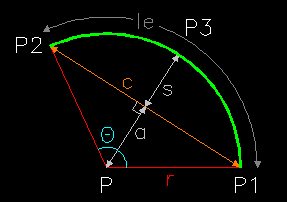
\includegraphics[width=0.5\textwidth]{figures/arcgeom.png}
	\captionof{figure}{Геометрия дуги окружности}
	\label{fig:arcgeom}
\end{figure}

Так как дуга окружности описывает часть этой окружности, то она и обладает всеми атрибутами данной окружности (см. рис. \ref{fig:arcgeom}). Среди них:

\begin{itemize}
	\item Радиус ($r$) --- радиус дуги такой же, как и у окружности;
	\item Центр ($P$) --- тот же, что и у окружности;
	\item Центральный угол ($\Theta$) --- в окружности равен $360^{\circ}$;
	\item Длина дуги ($le$) --- является частью периметра (длины) окружности.
\end{itemize}

Для дальнейшей работы с геометрией дуг примем, также, следующие специфичные атрибуты:

\begin{itemize}
	\item Начальная и конечная точка ($P1, P2$) --- это «вершины» дуги. Хотя иногда и целесообразно говорить о конкретных точках, не лежащих на концах дуги;
	\item Длина хорды ($c$) --- у дуг и окружностей можно провести бесконечное количество хорд, но для нас интерес представляет только хорда, проходящая через её вершины;
	\item Середина дуги ($P3$) --- точка, делящая дуги с данными вершинами на две, равные по длине, дуги;
	\item Апофема ($a$) --- это отрезок, вершинами которого являются середина дуги и её центр. Апофема перпендикулярна хорде;
	\item Высота дуги ($s$) --- это отрезок, проведённый из середины дуги перпендикулярно к хорде.
\end{itemize}

 Кроме самой себя, дуга может, также, и описывать другие геометрические формы: круговой сегмент и сектор. Обе геометрические формы включают в себя все вышеперечисленные атрибуты, однако для выведения формулы параметра \textit{bulge} (выпуклости), потребуется рассмотрение только кругового сектора.

В документации AutoCAD \cite{Autodesk} выпуклостью называется тангенс четверти угла дуги между выбранной вершиной и следующей вершиной в списках вершин полилиний. Отрицательность параметра \textit{bulge} указывает на то, что дуга отрисовывается по часовой стрелке от выбранной вершины к следующей. Выпуклость, равная нулю --- прямой сегмент, выпуклость, равная единице --- половина окружности.

Проблема «расшифровки» атрибутов дуги для дальнейших манипуляций с ней заключается в том, что входными данными являются только координаты вершин и рассматриваемый параметр --- \textit{bulge}.

В самом деле, взяв арктангенс от параметра \textit{bulge} и умножив его на $4$, легко получить центральный угол, на который опирается рассматриваемая дуга. Результат получен в радианах. Для перевода значения в градусы, необходимо умножить это значение на $\pi$ и разделить на $180^{\circ}$.

Для вывода данной зависимости, рассмотрим дугу окружности (см. рис. \ref{fig:arcchord}).

\begin{figure}[H]
	\centering
	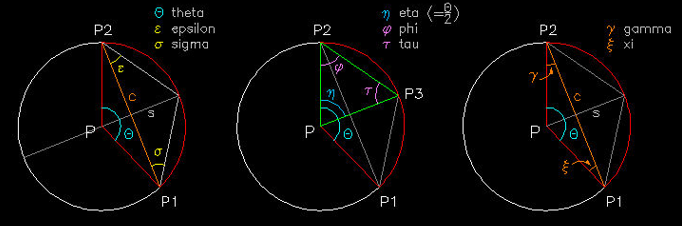
\includegraphics[width=1.0\textwidth]{figures/arcchord.png}
	\captionof{figure}{Дуга окружности с проведённой хордой и углами при ней}
	\label{fig:arcchord}
\end{figure}

Если провести к углу $\Theta$ биссектрису, то получится синий угол $\eta$. В итоге, мы получим равнобедренный треугольник (зеленый), в котором углы $\varphi$ и $\tau$ равны. Поскольку сумма углов в треугольнике всегда равна $180^{\circ}$ градусам, мы теперь знаем, что углы $\varphi$ и $\tau$ равны следующему (\ref{F:phi}):

\begin{equation}
	\varphi=\tau=\frac{(180^{\circ}-\frac{\Theta}{2})}{2}\Rightarrow\varphi=90^{\circ}-\frac{\Theta}{4}
	\label{F:phi}
\end{equation}

Теперь посмотрим на хорду $c$, проведённую от $P1$ до $P2$. Вместе с красными катетами угла $\Theta$ она тоже образует равнобедренный треугольник, а значит, $\gamma=\xi$. Угол при вершине треугольника $P-P1-P2$ --- это центральный угол $\Theta$, поэтому $\gamma$ и $\xi$ вычисляются следующим образом (\ref{F:gamma}):

\begin{equation}
	\gamma=\xi=\frac{180^{\circ}-\Theta}{2}\Rightarrow\gamma=90^{\circ}-\frac{\Theta}{2}
	\label{F:gamma}
\end{equation}

Таким образом, желтый угол $\varepsilon$ должен быть равняться разнице между фиолетовым углом $\varphi$ и оранжевым углом $\gamma$. Другими словами, $\varepsilon$ --- это четверть центрального угла $\Theta$ (\ref{F:epsilon}):

\begin{equation}
	\varepsilon=(90^{\circ}-\frac{\Theta}{4})-(90^{\circ}-\frac{\Theta}{2})\Rightarrow\varepsilon=\frac{\Theta}{2}-\frac{\Theta}{4}=\frac{\Theta}{4}
	\label{F:epsilon}
\end{equation}

Параметр \textit{bulge} (выпуклость) описывает, насколько дуга «выпирает» из вершин, то есть насколько велика высота дуги ($s$) (или расстояние от $P3$ до $P4$). Высота образует катет прямоугольного треугольника с углом, равным четверти центрального угла (см. желтый треугольник $P-P2-P3$ на рис. \ref{fig:epsilon}), и поскольку тангенс описывает отношение между катетами в прямоугольном треугольнике, легко описать геометрию с помощью этого одного угла (\ref{F:epsilon}):

\begin{equation}
	\frac{\sin(\varepsilon)}{\cos(\varepsilon)}=\tan(\varepsilon)
	\label{F:epsilon}
\end{equation}

\begin{figure}[H]
	\centering
	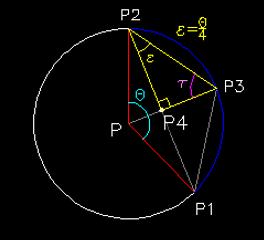
\includegraphics[width=0.5\textwidth]{figures/epsilon.png}
	\captionof{figure}{Связь угла $\varepsilon$ с центральным углом}
	\label{fig:epsilon}
\end{figure}

Мы, также, могли бы найти тангенс угла $\varepsilon$, просто разделив противолежащий катет на смежный катет --- что означает высоту дуги $s$, делённую на половину длины хорды $c$, --- но не зная $s$ и уже имея тангенс $\varepsilon$, полезнее найти $s$ (\ref{F:s}):

\begin{equation}
	s=\frac{c}{2}\cdot\tan(\varepsilon)
	\label{F:s}
\end{equation}

Примем

\begin{equation}
	\tan(\varepsilon)=bulge
	\label{F:tanepsilon}
\end{equation}

Тогда

\begin{equation}
	s=\frac{c}{2}\cdot bulge
	\label{F:sfinal}
\end{equation}

Таким образом, радиус дуги может быть найден следующим образом (\ref{F:r}):

\begin{equation}
	r=\frac{(\frac{c}{2})^2+s^2}{2s}
	\label{F:r}
\end{equation}

Знак той или иной выпуклости важен для определения дуги относительно вершин. Если выпуклость положительна, это означает, что дуга идёт против часовой стрелки от начальной вершины до конечной вершины. Если выпуклость отрицательна, это означает, что дуга идет, наоборот --- по часовой стрелке.

Поэтому все приведенные выше формулы должны касаться абсолютного значения выпуклости, а не фактического значения, иначе можно получить отрицательный радиус.

Итак, поняв, что $bulge = tan(\frac{\Theta}{4})$, в согласовании с документацией AutoCAD \cite{Autodesk} примем, что \textit{bulge} положителен, когда при передвижении от начальной точки дуги к конечной движение происходит против часовой стрелки.

Ясно, что когда $\Theta=0$, то и $bulge(\Theta)=0$. Для углов в $180^{\circ}$ условно принимается, что $bulge(\Theta)=\pm1$. В случае, когда $\Theta=90^{\circ}$, получим следующее (\ref{F:theta90}):

\begin{equation}
	bulge(90^{\circ})= \tan(\frac{90^{\circ}}{4})=\tan(\frac{\pi}{8})
	\label{F:theta90}
\end{equation}

Используя зависимость для тангенса половинного аргумента (\ref{F:tanhalfarg}):

\begin{equation}
	\tan(\frac{\alpha}{2})=\pm\frac{\sin(\frac{\alpha}{2})}{\cos(\frac{\alpha}{2})}=\pm\frac{2\sin^2(\frac{\alpha}{2})}{2\sin(\frac{\alpha}{2})\cos(\frac{\alpha}{2})}=\pm\frac{1-\cos(x)}{\sin(x)}
	\label{F:tanhalfarg}
\end{equation}

Для $\alpha=\frac{\pi}{8}$ получим (\ref{F:bulge90}):

\begin{equation}
	bulge(90^{\circ})=\tan(\frac{\pi}{8})=\pm\frac{1-\cos(\frac{\pi}{4})}{\sin(\frac{\pi}{4})}=\pm\frac{1-\frac{\sqrt2}{2}}{\frac{\sqrt2}{2}}=\pm\frac{1-\frac{1}{\sqrt2}}{\frac{1}{\sqrt2}}=\pm(\sqrt2-1)
	\label{F:bulge90}
\end{equation}



В результате, математические данные совпадают с документацией AutoCAD \cite{Autodesk} и гласят, что

\begin{enumerate}
	\item $bulge = 0$ для отрезка прямой,
	\item $bulge = \pm1$ для дуги в $180^{\circ}$ (половина окружности),
	\item $bulge = \pm(\sqrt2-1) \approx0.41421...$ для четвертей окружностей, когда угол раствора дуги равен $90^{\circ}$.
\end{enumerate}

%%% Local Variables:
%%% mode: latex
%%% TeX-master: "rpz"
%%% End:

%\chapter{Разработка программного обеспечения <<DXF Primiview>>}
\label{cha:design}

В данном разделе описывается процесс создания ПП для обработки геометрической информации 2D-объектов специального типа. Обосновывается выбор языка программирования, разрабатываются алгоритмы для разработки ПО, описывается процесс разработки конвертеров.

\section{Выбор языка программирования}

Для написания программы выбран язык программирования Python версии 3.11. Выбор языка программирования обоснован несколькими факторами.

\paragraph{Библиотеки.} Для создания описанного ПП необходимо привлечение различных библиотек. Кроме стандартной библиотеки, с Python можно использовать множество прикладных библиотек, несколько из которых будут описаны в следующих частях работы. Специфичные библиотеки, позволяющие <<читать>> DXF-файл и обрабатывать содержимое внутри него, написаны не для каждого ЯП. Библиотека <<eazy dxf>> для Python позволяет быстро и удобно выполнять данные операции.

\paragraph{Кроссплатформенность.} Большинство программ, написанных на Python, выполняются корректно на всех основных платформах. Перенос программы между операционными системами реализуется простым копированием кода. Кроме того, в процессе разработки ПО, для реализации пользовательского интерфейса используется набор расширений Qt, который тоже работает на таких платформах, как Linux и другие UNIX-подобные ОС, macOS и Windows.

\paragraph{Скорость и удобство разработки.} Удобочитаемсть, ясность и высокое качество этого языка позволяют повысить производительность разработчика во много раз, сравнивая, например, с компилирующими или строго типизированными языками, такими как C, C++ и Java. Объём программного кода на языке Python обычно составляет треть или даже пятую часть эквивалентного программного кода на языке C++ или Java. Кроме того, при запуске программы, написанной на ЯП Python минуются длинные этапы компиляции и связывания, необходимые в некоторых других ЯП, что, также, увеличивает производительность труда программиста \cite{learnpython3}.

\section{Разработка алгоритмов}

Для создания программного обеспечения необходимо сначала разработать концепцию функционирования программы, опираясь на её назначение, на основные её функции. Когда определены модули, блоки и функциональные части ПО, можно приступать к разработке его на выбранном ЯП.

\subsection{Структура программы}

Основываясь на цели, поставленной во введении, разрабатываемая утилита должна принимать на входе DXF-файл, то есть открывать его и обрабатывать его содержимое. Для проверки правильности обработанных данные, то есть, для верификации содержимого DXF-файла, программа должна визуализировать для пользователя обработанное. После верификации обработанных данных и, соответственно, подтверждения соответствия их исходным, пользователю должна предоставляться возможность конвертировать эти данные в какой-либо из предлагаемых форматов. За это отвечает модуль экспорта, который, в свою очередь, подразделяется на четыре модуля, отвечающие за преобразование данных в различные форматы. Среди них следующие:

\begin{enumerate}
	\item Модуль экспорта в TXT-файл, где данные будут представлены в такой же форме, как и в оригинальном DXF-файле, за исключением того, что содержаться в нём будут только поддерживаемые сущности (LINE, POLYLINE, ARC, CIRCLE).
	\item Модуль экспорта в TXT-файл, в котором поддерживаемые сущности будут представлены сочетанием двух строк, первая из которых --- начальная точка примитива, вторая --- конечная. Вторая строка содержит в себе радиус скругления примитива, переходящего из первой точки во вторую.
	\item Модуль экспорта в формат SVG, который, при открытии, векторно отображает информацию в нём.
	\item Модуль экспорта JSON-формат. В данном формате, по подобию формату TXT (x, y, r), содержаться точки, олицетворяющие начало и конец того или иного примитива. В данном случае информация в файле тэгированная, что означает, что в дальнейшем несложно будет получить желаемые куски данных из потенциально объёмного JSON-файла путём обращения по желаемому тэгу.
\end{enumerate}


Схему, отображающую основное содержание разрабатываемого ПО, можно наблюдать на рисунке \ref{fig:organisationsdiagramm}.

\begin{figure}[H]
	\centering
	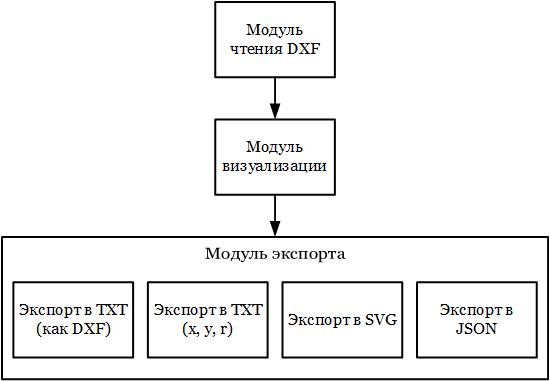
\includegraphics[width=0.8\textwidth]{figures/organisationsdiagramm.png}
	\captionof{figure}{Принципиальная структура ПО <<Primiview>>}
	\label{fig:organisationsdiagramm}
\end{figure}


\subsection{Алгоритмы модулей программы}

В данном пункте приводится описание алгоритмов ПО <<Primiview>> в виде псевдокода.

\paragraph{Алгоритм чтения DXF-файлов.} Алгоритм \ref{alg:readdxf} показывает схему работы процесса извлечения поддерживаемых ПО Primiview примитивов из выбранного DXF-файла.

На первой итерации осуществляется разбиение блоков, в которых могут быть <<спрятаны>> остальные сущности. В случае, если пропустить данный этап, то объекты, находящиеся внутри блоков не будут видны библиотекой \textit{ezdxf}, которая используется для чтения DXF-файлов.

После <<разрушения>> всех блоков примитивы становятся <<видимыми>>. Далее запускается цикл, итерирующий объекты пространства объектов модели (\textit{modelspace}). В случае совпадения объекта с одной из поддерживаемых сущностей, она сохраняется в список соответствующих объектов в оперативной памяти программы. Списком далее будет называться изменяемый упорядоченный тип данных, представляющих собой последовательность элементов, разделённых между собой запятой и заключённых в квадратные скобки. Данный тип данных используется в ЯП Python, поэтому для соблюдения общности, термин будет применяться и в части \ref{sec:software} этого раздела.

Примем ряд условных обозначений:

$msp$ --- пространство объектов модели (modelspace);

$\dashrightarrow$ --- запись объекта в множество.


\begin{algorithm}[H]
	\SetAlgoLined
	\KwData{путь к DXF-файлу}
	\KwResult{массивы примитивов и информации о них в оперативной памяти программы}
	инициализация;
		
	\For{$\forall$ сущн. типа Вставка (INSERT) $\in msp$}{разбиение сущности}
	
	\For{$\forall$ сущн. $\in msp$}{
		\If{сущ явл. линией}{сущн. $\dashrightarrow$ множ. линий}
		\ElseIf{сущн. явл. дугой}{сущн. $\dashrightarrow$ множ. дуг}
		\ElseIf{сущн. явл. окружностью}{сущн. $\dashrightarrow$ множ. окружностей}
		\ElseIf{сущн. явл. полилинией}{сущн. $\dashrightarrow$ множ. полилиний}
	}
	
	\caption[Сохранение поддерживаемых примитивов; из DXF в оперативную память программы]
	{\tabular[t]{@{}l@{}}Сохранение поддерживаемых примитивов \\ из DXF в оперативную память программы\endtabular}
	\label{alg:readdxf}
\end{algorithm}

\paragraph{Алгоритм записи примитивов в TXT (как DXF).} Принцип данного алгоритма (см. алгоритм \ref{alg:dxfintotxt}) основан на открытии созданного TXT-файла, а после --- перебора прочитанных из DXF примитивов и записи из каждого из них необходимой информации в открытый для редактирования TXT-файл.

Записи в текстовом файле должны выглядеть следующим образом (см. листинг \ref{list:txtdxfsicht}):
%\begin{verbatim}
%	LINE(#01)
%	0.1 0.1
%	0.1 0.1
%\end{verbatim}

\begin{lstlisting}[caption={Пример содержания TXT-файла (как DXF)},label=list:txtdxfsicht]
	LINE(#01)
	0.1 0.1
	0.1 0.1
\end{lstlisting}

\begin{algorithm}[H]
	\SetAlgoLined
	\KwData{путь к имя.txt}
	\KwResult{имя.txt (как DXF)}
	инициализация;
	
	\For{$\forall$ LINE $\in$ множ. линий}{записать в файл: атрибут сущности, $x_0, y_0$, $x_1, y_1$; перевести курсор на новую строку}
	
	\For{$\forall$ ARC $\in$ множ. дуг}{записать в файл: атрибут сущности, $x_0, y_0$, $x_1, y_1$, $r$; перевести курсор на новую строку}
	
	\For{$\forall$ CIRCLE $\in$ множ. окруж.}{записать в файл: атрибут сущности, $x_c, y_c$, $r$; перевести курсор на новую строку}
	
	\For{$\forall$ LWPOLYLINE $\in$ множ. полилин.}{записать в файл атрибут сущности;
		
		\For{$\forall$ точки LWPOLYLINE}{
			
			\For{$\forall$ координаты x, y}{записать в файл значение координаты}
			}
		перевести курсор на новую строку}
	\caption{Запись примитивов в TXT (как DXF)}
	\label{alg:dxfintotxt}
\end{algorithm}

В алгоритме \ref{alg:dxfintotxt} $x_0, y_0$ --- координаты начала примитива; $x_1, y_1$ --- координаты конца примитива; $x_c, y_c$ --- координаты центра окружности; $r$ --- радиус дуги или окружности.

\paragraph{Алгоритм записи примитивов в TXT (x,y,r).} Алгоритм \ref{alg:primsintotxt} призван, так же как и в прошлом случае, в открытый только что созданный текстовый файл записать информацию о примитивах, которые были прочитаны из выбранного DXF-файла.

Записи в текстовом файле должны выглядеть следующим образом (см. листинг \ref{list:primsdxfsicht}):
%\begin{verbatim}
%	1.52 1.86 0
%	1.12 2.08 0
%	1.16 2.04 4.0
%	...
%\end{verbatim}

\begin{lstlisting}[caption={Пример содержания TXT-файла (x, y, r)},label=list:primsdxfsicht]
	1.52 1.86 0
	1.12 2.08 0
	1.16 2.04 4.0
	...
\end{lstlisting}

Полилиния может содержать в себе, как отрезки, так и дуги. В объектах LWPOINT сущности LWPOLYLINE степень искривления показывает параметр \textit{bulge}, суть которого подробно описана в разделе \ref{sec:allaboutdxf}. Так как желаемый формат вывода информации о примитивах содержит именно радиус примитива, а не параметр искривления, то необходимо удобно получить радиус из \textit{bulge}.

Для этого воспользуемся уже выведенной зависимостью \cite{ukoloff} и применим её в принятых обозначениях (\ref{F:rad}):

\begin{equation}
	R=|bulge+\frac{1}{bulge}|\cdot\frac{|A-Z|}{4},
	\label{F:rad}
\end{equation}

где A --- начальная точка;

Z --- конечная точка.

Примем, что $A(x_0,y_0), B(x_1,y_1)$. Тогда $AZ(x_1-x_0; y_1-y_0)$.
Таким образом, длина вектора через декартовы координаты (\ref{F:veclen}):
\begin{equation}
	|A-Z|=\sqrt{(x_1-x_0)^2+(y_1-y_0)^2}
	\label{F:veclen}
\end{equation}


\begin{algorithm}[H]
	\SetAlgoLined
	\KwData{текущая точка, следующая точка}
	\KwResult{радиус сегмента полилинии}
	инициализация;
	
	\If{$bulge$ (текущей точки) $=0$}{$r=0$}	
	\Else{$r=|bulge+\frac{1}{bulge}|\cdot\frac{\sqrt{(x_{nexP}-x_{prevP})^2+(y_{nexP}-y_{prevP})^2}}{4}$}
	
	\caption{Вычисление радиуса сегмента полилинии}
	\label{alg:polyarcrad}
\end{algorithm}

Примем условные обозначения:

$\rightsquigarrow$ --- запись в файл;

$newline$ --- перевод на новую строку.

\begin{algorithm}[H]
	\SetAlgoLined	
	\KwData{путь к имя.txt}
	\KwResult{имя.txt (x,y,r)}	
	\ForEach{LINE $\in$ множ. линий}{$x_0 \quad y_0 \quad 0\rightsquigarrow$ имя.txt; \quad $x_1 \quad y_1 \quad 0 \rightsquigarrow$ имя.txt}
	
	\ForEach{ARC $\in$ множ. дуг}{$x_0 \quad y_0 \quad 0\rightsquigarrow$ имя.txt; \quad $x_1 \quad y_1 \quad r \rightsquigarrow$ имя.txt}
	
	\ForEach{CIRCLE $\in$ множ. окруж.}{$x_c + r \quad y_c \quad 0\rightsquigarrow$ имя.txt\tcc*{первая половина окруж.} $x_c - r \quad y_c \quad r \rightsquigarrow$ имя.txt \\  $x_c - r \quad y_c \quad 0 \rightsquigarrow$ имя.txt\tcc*{вторая половина окруж.} $x_c + r \quad y_c \quad r \rightsquigarrow$ имя.txt} \ForEach{POLYLINE $\in$ множ. полилиний \\ prevPoint=None \tcc*{предыдущая точка}}{
		\ForEach{LWPOINT $\in$ множ. точек. полилинии}{
			\If{prevPoint$\neq$None}{r = алгоритм \ref{alg:polyarcrad} (prevPoint, LWPOINT)
			$x(prevP) \quad y(prevP) \quad 0 \rightsquigarrow$ имя.txt\\
			$x(lwpoint) \quad y(lwpoint) \quad r \rightsquigarrow$ имя.txt
			}
		$prevPoint = lwpoint$
		} \newpage
		\If{контур замкнут}{
		r = алгоритм \ref{alg:polyarcrad} (prevPoint, LWPOINT) \\
		$x(lwpoint_\text{посл}) \quad y(lwpoint_\text{посл}) \quad 0 \rightsquigarrow$ имя.txt\\
		$x(lwpoint_\text{перв}) \quad y(lwpoint_\text{перв}) \quad r \rightsquigarrow$ имя.txt
		}
	}
	\caption{Запись примитивов в TXT (x, y, r)}
	\label{alg:primsintotxt}
\end{algorithm}

\paragraph{Алгоритм записи примитивов в SVG.} Формирования файла типа SVG отличается от предыдущих двух, так как этот формат представляет собой язык разметки, а значит, имеет правила синтаксиса, грамматики и т.д. Это расширение языка разметки XML, поэтому в начале, в преамбуле, указывается версия XML, кодировка символов и указание синтаксическому анализатору об игнорировании любых объявлений разметки в определении типа документа.

\begin{lstlisting}[language=XML,caption={Первая строка SVG-файлов},label=list:1stsvgline]
	<?xml version="1.0" encoding="UTF-8" standalone="no"?>
\end{lstlisting}

Следующие две строки должны содержать определение типа документа (заголовок DOCTYPE), однако, данное объявление может оказаться источником ошибок при применении в браузере Mozilla Firefox. Поэтому вместо этого используется атрибут \Code{baseProfile} со значением <<full>> внутри элемента <svg>.

Начиная с четвёртой строки объявляется корневой элемент <svg>:

\begin{lstlisting}[language=XML,caption={Первая строка SVG-файлов},label=list:4thsvgline]
	<svg version="1.1" width="100%" height="100%"
	viewBox="102.1188828597992 -211.7921423734452 50.000000000000014 26.0"
	baseProfile="full"
	xmlns="http://www.w3.org/2000/svg"
	xmlns:xlink="http://www.w3.org/1999/xlink"
	xmlns:ev="http://www.w3.org/2001/xml-events">
\end{lstlisting}

В листинге \ref{list:4thsvgline} присутствует необязательный элемент \Code{viewBox}, который представляет собой параметр с четырьмя значениями, отделяемыми пробелами, определяющими квадратную рамку, в которой будет располагаться графика. Данный атрибут позволяет автоматически масштабировать изображение до размеров указанного контейнера, причём, без потери качества, так как графическая информация храниться и воспроизводится в векторном формате.

Первые два значение --- минимальные координаты $x$ и $y$ рамки, в которой располагается изображение. Третье и четвёртое значения --- соответственно, ширина и высота рамки, в которой находится изображение. Значения указываются в пикселях.

Таким образом, чтобы перенести данные из DXF в SVG, сначала определяются эти четыре значения. Алгоритмы для их определения: алгоритм \ref{alg:allcoords}, алгоритм \ref{alg:extremums} и алгоритм \ref{alg:dimes}.

\begin{algorithm}[H]
	\SetAlgoLined
	\KwData{списки примитивов с параметрами}
	\KwResult{список координат $x$, список координат $y$}
	инициализация; пустой список координат $x$, пустой список координат $y$
	\For{$\forall$ LINE $\in$ множ. линий}{$x_0,x_1\dashrightarrow$ список $x$\\$y_0,y_1\dashrightarrow$ список $y$}
	
	\For{$\forall$ ARC $\in$ множ. дуг}{$(x_c+r),(x_c-r)\dashrightarrow$ список $x$\\$(y_c+r),(y_c+r)\dashrightarrow$ список $y$}
	
	\For{$\forall$ CIRCLE $\in$ множ. окруж.}{$(x_c+r),(x_c-r)\dashrightarrow$ список $x$\\$(y_c+r),(y_c+r)\dashrightarrow$ список $y$}
	
	\For{$\forall$ LWPOLYLINE $\in$ множ. полилин.}{
		\For{$\forall$точки в множ. LWPOINTS}{
		$x\dashrightarrow$ список $x$\\$y\dashrightarrow$ список $y$}}
	вернуть список координат $x$ и список координат $y$
	\caption{Вычленение координат изображения из DXF в отдельные списки}
	\label{alg:allcoords}
\end{algorithm}

\begin{algorithm}[H]
	\SetAlgoLined
	\KwData{список координат $x$, список координат $y$}
	\KwResult{$x_{MIN}, y_{MIN}$}
	инициализация;\\
	использовать алгоритм \ref{alg:allcoords}\\
	вернуть $x_{MIN}, y_{MIN}$ из списков стандартными функциями сортировки ЯП
	\caption{Поиск наименьших координат изображения из DXF}
	\label{alg:extremums}
\end{algorithm}

\begin{algorithm}[H]
	\SetAlgoLined
	\KwData{список координат $x$, список координат $y$}
	\KwResult{ширина и высота рамки изображения}
	инициализация;
	использовать алгоритм \ref{alg:allcoords}\\
	определить $x_{MIN}, x_{MAX}, y_{MIN}, y_{MAX}$ из списков стандартными функциями сортировки ЯП\\
	ширина $=x_{MAX}-x_{MIN}$\\
	высота $=y_{MAX}-y_{MIN}$\\
	вернуть значения ширины и высоты
	\caption{Поиск длины и высоты изображения из DXF}
	\label{alg:dimes}
\end{algorithm}





\section{Разработка программного обеспечения}\label{sec:software}


%%% Local Variables:
%%% mode: latex
%%% TeX-master: "rpz"
%%% End:


\backmatter %% Здесь заканчивается нумерованная часть документа и начинаются ссылки и
            %% заключение

\Conclusion % заключение к отчёту

В соответствии с целью и задачами выпускной квалификационной работы получены следующие результаты:

\begin{enumerate}[1)]
	\item Проверены, сведены в одной работе, а также, в целях, возникших при разработке алгоритмов и кода ПО, выведены  математические зависимости между параметром выпуклости (\textit{bulge}) и радиусом, углом раствора, координатами концов, координатами центра, и другими геометрическими параметрами дуги окружности;
	\item Разработаны алгоритмы конвертации формата DXF в форматы TXT(DXF-type), TXT(x,y,r), SVG, JSON по определённым правилам;
	\item Разработаны алгоритмы по нахождению геометрических параметров чертежа в DXF (список всех координат, габариты чертежа, наименьшие координаты), а также объектов DXF (радиус сегмента полилинии, центр дуги, радиус дуги по параметру \textit{bulge});
	\item Разработаны конвертеры из формата DXF в форматы TXT(DXF-type), TXT(x,y,r), SVG, JSON в виде программного обеспечения <<primiview>> на ЯП Python:
	\begin{enumerate}[4.1)]
		\item Разработана архитектура внутренней репрезентации примитивов DXF в программе <<primiview>>;
		\item Разработаны модули визуализации поддерживаемый объектов DXF, конвертации форматов;
		\item Разработан пользовательский интерфейс с помощью библиотеки PyQt;
		\item Проведено ручное тестирование программного обеспечения, в ходе которого была подтверждена корректность конвертации выбранных типов объектов DXF в указанные форматы.
	\end{enumerate}
	\item Проведён экономический расчёт:
	\begin{enumerate}[5.1)]
		\item Разработана экономическая модель проекта;
		\item Построено дерево задач, необходимых для выполнения целей проекта;
		\item Построена диаграмма Ганта и сетевой график,  в результате которых проект спланирован для реализации за 230 календарных дней;
		\item Проведён анализ сравнительной экономической эффективности проекта.
	\end{enumerate}
\end{enumerate}

\paragraph{Перспективы дальнейшей работы над проектом} 
\nopagebreak

Можно выделить следующие направления дальнейшего развития и совершенствования программного обеспечения <<primiview>> по конвертации форматов для обработки геометрической информации 2D-объектов:

\begin{enumerate}[1)]
	\item Расширение поддерживаемых для чтения и конвертации объектов DXF-файлов, например поддержка сплайнов, эллипсов, надписей;
	\item Создание поддержки распознавания и конвертации приложением типов, толщины и цветов линий;
	\item Расширение поддерживаемых входных форматов для конвертации, например Autodesk-форматов: DWG, DWS, DWT; Компас3D-форматов: FRW, FRT, CDW, CDT; DSS SolidWorks-форматов: DRW, SLDDRW, DRWDOT;
	\item Создание новых конвертеров для преобразования DXF, например в формат языка разметки YAML. Полезным и пока ещё нереализованным может быть конвертация во фрагменты формата TEX на языке создания графики в \TeX-среде --- Tikz. Также, удобными для дальнейшей работы форматами, в которые необходима конвертация DXF могут быть форматы векторной и растровой графики: PDF, GIF, PNG, JPEG.
\end{enumerate}


%%% Local Variables: 
%%% mode: latex
%%% TeX-master: "rpz"
%%% End: 


% % Список литературы при помощи BibTeX
% Юзать так:
%
% pdflatex rpz
% bibtex rpz
% pdflatex rpz

\bibliographystyle{gost780u}
\bibliography{00_vkr}

%%% Local Variables: 
%%% mode: latex
%%% TeX-master: "rpz"
%%% End: 


%\appendix   % Тут идут приложения

%\chapter{Текстовые результаты конвертации}
\label{cha:appendix1}

\lstinputlisting[caption=Результат конвертации тестового DXF с дугами в TXT(DXF-type),label=lst:all_arcs_dxftype]{listings/all_arcs_dxftype.txt}

\lstinputlisting[caption=Результат конвертации тестового DXF с дугами в TXT(xyr),label=lst:all_arcs_txtxyr]{listings/all_arcs_xyr.txt}

\lstinputlisting[language=XML,caption=Результат конвертации тестового DXF с дугами в SVG,label=lst:all_arcs_svg]{listings/all_arcs.svg}

\lstinputlisting[,caption=Результат конвертации тестового DXF с дугами в JSON,label=lst:all_arcs_json]{listings/all_arcs.json}

%%% Local Variables: 
%%% mode: latex
%%% TeX-master: "rpz"
%%% End: 

%%\chapter{Еще картинки}
%\label{cha:appendix2}
%
%\begin{figure}
%\centering
%\caption{Еще одна картинка, ничем не лучше предыдущей. Но надо же как-то заполнить место.}
%\end{figure}

%%% Local Variables: 
%%% mode: latex
%%% TeX-master: "rpz"
%%% End: 


\end{document}

%%% Local Variables:
%%% mode: latex
%%% TeX-master: t
%%% End:
